\documentclass[twoside]{book}

% Packages required by doxygen
\usepackage{fixltx2e}
\usepackage{calc}
\usepackage{doxygen}
\usepackage[export]{adjustbox} % also loads graphicx
\usepackage{graphicx}
\usepackage[utf8]{inputenc}
\usepackage{makeidx}
\usepackage{multicol}
\usepackage{multirow}
\PassOptionsToPackage{warn}{textcomp}
\usepackage{textcomp}
\usepackage[nointegrals]{wasysym}
\usepackage[table]{xcolor}

% NLS support packages
\usepackage[french]{babel}

% Font selection
\usepackage[T1]{fontenc}
\usepackage[scaled=.90]{helvet}
\usepackage{courier}
\usepackage{amssymb}
\usepackage{sectsty}
\renewcommand{\familydefault}{\sfdefault}
\allsectionsfont{%
  \fontseries{bc}\selectfont%
  \color{darkgray}%
}
\renewcommand{\DoxyLabelFont}{%
  \fontseries{bc}\selectfont%
  \color{darkgray}%
}
\newcommand{\+}{\discretionary{\mbox{\scriptsize$\hookleftarrow$}}{}{}}

% Page & text layout
\usepackage{geometry}
\geometry{%
  a4paper,%
  top=2.5cm,%
  bottom=2.5cm,%
  left=2.5cm,%
  right=2.5cm%
}
\tolerance=750
\hfuzz=15pt
\hbadness=750
\setlength{\emergencystretch}{15pt}
\setlength{\parindent}{0cm}
\setlength{\parskip}{3ex plus 2ex minus 2ex}
\makeatletter
\renewcommand{\paragraph}{%
  \@startsection{paragraph}{4}{0ex}{-1.0ex}{1.0ex}{%
    \normalfont\normalsize\bfseries\SS@parafont%
  }%
}
\renewcommand{\subparagraph}{%
  \@startsection{subparagraph}{5}{0ex}{-1.0ex}{1.0ex}{%
    \normalfont\normalsize\bfseries\SS@subparafont%
  }%
}
\makeatother

% Headers & footers
\usepackage{fancyhdr}
\pagestyle{fancyplain}
\fancyhead[LE]{\fancyplain{}{\bfseries\thepage}}
\fancyhead[CE]{\fancyplain{}{}}
\fancyhead[RE]{\fancyplain{}{\bfseries\leftmark}}
\fancyhead[LO]{\fancyplain{}{\bfseries\rightmark}}
\fancyhead[CO]{\fancyplain{}{}}
\fancyhead[RO]{\fancyplain{}{\bfseries\thepage}}
\fancyfoot[LE]{\fancyplain{}{}}
\fancyfoot[CE]{\fancyplain{}{}}
\fancyfoot[RE]{\fancyplain{}{\bfseries\scriptsize Généré par Doxygen }}
\fancyfoot[LO]{\fancyplain{}{\bfseries\scriptsize Généré par Doxygen }}
\fancyfoot[CO]{\fancyplain{}{}}
\fancyfoot[RO]{\fancyplain{}{}}
\renewcommand{\footrulewidth}{0.4pt}
\renewcommand{\chaptermark}[1]{%
  \markboth{#1}{}%
}
\renewcommand{\sectionmark}[1]{%
  \markright{\thesection\ #1}%
}

% Indices & bibliography
\usepackage{natbib}
\usepackage[titles]{tocloft}
\setcounter{tocdepth}{3}
\setcounter{secnumdepth}{5}
\makeindex

% Hyperlinks (required, but should be loaded last)
\usepackage{ifpdf}
\ifpdf
  \usepackage[pdftex,pagebackref=true]{hyperref}
\else
  \usepackage[ps2pdf,pagebackref=true]{hyperref}
\fi
\hypersetup{%
  colorlinks=true,%
  linkcolor=blue,%
  citecolor=blue,%
  unicode%
}

% Custom commands
\newcommand{\clearemptydoublepage}{%
  \newpage{\pagestyle{empty}\cleardoublepage}%
}

\usepackage{caption}
\captionsetup{labelsep=space,justification=centering,font={bf},singlelinecheck=off,skip=4pt,position=top}

%===== C O N T E N T S =====

\begin{document}

% Titlepage & ToC
\hypersetup{pageanchor=false,
             bookmarksnumbered=true,
             pdfencoding=unicode
            }
\pagenumbering{alph}
\begin{titlepage}
\vspace*{7cm}
\begin{center}%
{\Large Othello\+\_\+\+Algo\+\_\+19-\/20\+\_\+12 }\\
\vspace*{1cm}
{\large Généré par Doxygen 1.8.13}\\
\end{center}
\end{titlepage}
\clearemptydoublepage
\pagenumbering{roman}
\tableofcontents
\clearemptydoublepage
\pagenumbering{arabic}
\hypersetup{pageanchor=true}

%--- Begin generated contents ---
\chapter{Index des classes}
\section{Liste des classes}
Liste des classes, structures, unions et interfaces avec une brève description \+:\begin{DoxyCompactList}
\item\contentsline{section}{\hyperlink{structCouleur}{Couleur} \\*Le type \hyperlink{structCouleur}{Couleur} permet de symboliser un pion }{\pageref{structCouleur}}{}
\item\contentsline{section}{\hyperlink{structCoup}{Coup} \\*Le type \hyperlink{structCoup}{Coup} permet de jouer une couleur à une position }{\pageref{structCoup}}{}
\item\contentsline{section}{\hyperlink{structCoups}{Coups} \\*Le type \hyperlink{structCoups}{Coups} permet de stocker plusieurs \hyperlink{structCoup}{Coup} }{\pageref{structCoups}}{}
\item\contentsline{section}{\hyperlink{structJoueur}{Joueur} \\*Le type \hyperlink{structJoueur}{Joueur} permet de manipuler une couleur en sachant si elle est jouée par une IA ou un \hyperlink{structJoueur}{Joueur} réel }{\pageref{structJoueur}}{}
\item\contentsline{section}{\hyperlink{structPosition}{Position} \\*Le type \hyperlink{structPosition}{Position} permet de symboliser les cases du plateau }{\pageref{structPosition}}{}
\end{DoxyCompactList}

\chapter{Index des fichiers}
\section{Liste des fichiers}
Liste de tous les fichiers documentés avec une brève description \+:\begin{DoxyCompactList}
\item\contentsline{section}{include/\hyperlink{Affichage_8h}{Affichage.\+h} \\*Fichier contenant les fonctions d\textquotesingle{}affichage }{\pageref{Affichage_8h}}{}
\item\contentsline{section}{include/\hyperlink{Colonne_8h}{Colonne.\+h} \\*Fichier contenant la définition de l\textquotesingle{}enum Colonne et de ses fonctions associées }{\pageref{Colonne_8h}}{}
\item\contentsline{section}{include/\hyperlink{Couleur_8h}{Couleur.\+h} \\*Fichier contenant la définition du type \hyperlink{structCouleur}{Couleur}, l\textquotesingle{}enum nom\+Couleur et de leurs fonctions associées }{\pageref{Couleur_8h}}{}
\item\contentsline{section}{include/\hyperlink{Coup_8h}{Coup.\+h} \\*Fichier contenant la définition du type \hyperlink{structCoup}{Coup} et de ses fonctions associées }{\pageref{Coup_8h}}{}
\item\contentsline{section}{include/\hyperlink{Coups_8h}{Coups.\+h} \\*Fichier contenant la définition du type \hyperlink{structCoups}{Coups} et de ses fonctions associées }{\pageref{Coups_8h}}{}
\item\contentsline{section}{include/\hyperlink{Direction_8h}{Direction.\+h} \\*Fichier contenant la définition de l\textquotesingle{}enum Direction et de ses fonctions associées }{\pageref{Direction_8h}}{}
\item\contentsline{section}{include/\hyperlink{GererPartie_8h}{Gerer\+Partie.\+h} \\*Fichier contenant la définition des fonctions permettant de gérer le déroulement d\textquotesingle{}une partie d\textquotesingle{}Othello }{\pageref{GererPartie_8h}}{}
\item\contentsline{section}{include/\hyperlink{IntelligenceArtificielle_8h}{Intelligence\+Artificielle.\+h} \\*Fichier contenant la définition des fonctions pour obtenir un \hyperlink{structCoup}{Coup} d\textquotesingle{}une IA }{\pageref{IntelligenceArtificielle_8h}}{}
\item\contentsline{section}{include/\hyperlink{Joueur_8h}{Joueur.\+h} \\*Fichier contenant la définition du type \hyperlink{structJoueur}{Joueur} et de ses fonctions associées }{\pageref{Joueur_8h}}{}
\item\contentsline{section}{include/\hyperlink{Ligne_8h}{Ligne.\+h} \\*Fichier contenant la définition de l\textquotesingle{}enum Ligne et de ses fonctions associées }{\pageref{Ligne_8h}}{}
\item\contentsline{section}{include/\hyperlink{Menu_8h}{Menu.\+h} \\*Fichier contenant la définition les fonctions utilisées par les fichiers Menu\+Graphique et Menu\+Ligne\+Commande }{\pageref{Menu_8h}}{}
\item\contentsline{section}{include/\hyperlink{MenuGraphique_8h}{Menu\+Graphique.\+h} \\*Fichier contenant la définition de fonctions permettant d\textquotesingle{}avoir un menu graphique pour lancer le jeu }{\pageref{MenuGraphique_8h}}{}
\item\contentsline{section}{include/\hyperlink{MenuLigneCommande_8h}{Menu\+Ligne\+Commande.\+h} \\*Fichier contenant la définition de fonctions permettant d\textquotesingle{}avoir un menu en ligne de commande pour lancer le jeu }{\pageref{MenuLigneCommande_8h}}{}
\item\contentsline{section}{include/\hyperlink{Othello_8h}{Othello.\+h} \\*Fichier contenant la définition du main du programme }{\pageref{Othello_8h}}{}
\item\contentsline{section}{include/\hyperlink{ParcourirDirection_8h}{Parcourir\+Direction.\+h} \\*Fichier contenant la définition de fonctions pour parcourir un plateau dans des directions données et voir si un coup est possible }{\pageref{ParcourirDirection_8h}}{}
\item\contentsline{section}{include/\hyperlink{Plateau_8h}{Plateau.\+h} \\*Fichier contenant la définition des fonctions permettant d\textquotesingle{}intéragir avec le plateau de jeu }{\pageref{Plateau_8h}}{}
\item\contentsline{section}{include/\hyperlink{Position_8h}{Position.\+h} \\*Fichier contenant la définition du type \hyperlink{structPosition}{Position} et de ses fonctions associées }{\pageref{Position_8h}}{}
\item\contentsline{section}{include/\hyperlink{RechercherCoup_8h}{Rechercher\+Coup.\+h} \\*Fichier contenant la définition des fonctions pour rechercher des \hyperlink{structCoup}{Coup} possibles }{\pageref{RechercherCoup_8h}}{}
\end{DoxyCompactList}

\chapter{Documentation des classes}
\hypertarget{structCouleur}{}\section{Référence de la structure Couleur}
\label{structCouleur}\index{Couleur@{Couleur}}


Le type \hyperlink{structCouleur}{Couleur} permet de symboliser un pion.  




{\ttfamily \#include $<$Couleur.\+h$>$}

\subsection*{Attributs publics}
\begin{DoxyCompactItemize}
\item 
\hyperlink{Couleur_8h_aaca4e6192fa64673e34ef06ceb76bb16}{nom\+Couleur} \hyperlink{structCouleur_a0083f38ad28cc4b9ca57356fa0440ee9}{nom}
\begin{DoxyCompactList}\small\item\em Nom de la couleur. \end{DoxyCompactList}\item 
char \hyperlink{structCouleur_a4da2f2ca44f4b0c7c963afd7339f2600}{symbole}
\begin{DoxyCompactList}\small\item\em Symbole représentant la couleur. \end{DoxyCompactList}\end{DoxyCompactItemize}


\subsection{Description détaillée}
Le type \hyperlink{structCouleur}{Couleur} permet de symboliser un pion. 

La couleur possède un nom et un symbole, le symbole est utilisé lors des affichages pour représenter la couleur. 

\subsection{Documentation des données membres}
\mbox{\Hypertarget{structCouleur_a0083f38ad28cc4b9ca57356fa0440ee9}\label{structCouleur_a0083f38ad28cc4b9ca57356fa0440ee9}} 
\index{Couleur@{Couleur}!nom@{nom}}
\index{nom@{nom}!Couleur@{Couleur}}
\subsubsection{\texorpdfstring{nom}{nom}}
{\footnotesize\ttfamily \hyperlink{Couleur_8h_aaca4e6192fa64673e34ef06ceb76bb16}{nom\+Couleur} Couleur\+::nom}



Nom de la couleur. 

\mbox{\Hypertarget{structCouleur_a4da2f2ca44f4b0c7c963afd7339f2600}\label{structCouleur_a4da2f2ca44f4b0c7c963afd7339f2600}} 
\index{Couleur@{Couleur}!symbole@{symbole}}
\index{symbole@{symbole}!Couleur@{Couleur}}
\subsubsection{\texorpdfstring{symbole}{symbole}}
{\footnotesize\ttfamily char Couleur\+::symbole}



Symbole représentant la couleur. 



La documentation de cette structure a été générée à partir du fichier suivant \+:\begin{DoxyCompactItemize}
\item 
include/\hyperlink{Couleur_8h}{Couleur.\+h}\end{DoxyCompactItemize}

\hypertarget{structCoup}{}\section{Référence de la structure Coup}
\label{structCoup}\index{Coup@{Coup}}


Le type \hyperlink{structCoup}{Coup} permet de jouer une couleur à une position.  




{\ttfamily \#include $<$Coup.\+h$>$}



Graphe de collaboration de Coup\+:
\nopagebreak
\begin{figure}[H]
\begin{center}
\leavevmode
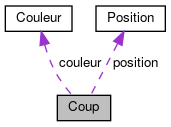
\includegraphics[width=200pt]{structCoup__coll__graph}
\end{center}
\end{figure}
\subsection*{Attributs publics}
\begin{DoxyCompactItemize}
\item 
\hyperlink{structPosition}{Position} \hyperlink{structCoup_a53a5b29ee8fde3fa1c9fbc220e2f5a56}{position}
\begin{DoxyCompactList}\small\item\em \hyperlink{structPosition}{Position} où le \hyperlink{structCoup}{Coup} doit être joué. \end{DoxyCompactList}\item 
\hyperlink{structCouleur}{Couleur} \hyperlink{structCoup_a6abc44ab931a3ff7d12b475f5af460f3}{couleur}
\begin{DoxyCompactList}\small\item\em \hyperlink{structCouleur}{Couleur} du joueur qui joue le \hyperlink{structCoup}{Coup}. \end{DoxyCompactList}\end{DoxyCompactItemize}


\subsection{Description détaillée}
Le type \hyperlink{structCoup}{Coup} permet de jouer une couleur à une position. 

Le \hyperlink{structCoup}{Coup} est composé d\textquotesingle{}une position et d\textquotesingle{}une couleur. Lorsque ce \hyperlink{structCoup}{Coup} est considéré comme joué, alors la couleur qu\textquotesingle{}il contient est insérée à la position donnée sur le plateau de jeu. 

\subsection{Documentation des données membres}
\mbox{\Hypertarget{structCoup_a6abc44ab931a3ff7d12b475f5af460f3}\label{structCoup_a6abc44ab931a3ff7d12b475f5af460f3}} 
\index{Coup@{Coup}!couleur@{couleur}}
\index{couleur@{couleur}!Coup@{Coup}}
\subsubsection{\texorpdfstring{couleur}{couleur}}
{\footnotesize\ttfamily \hyperlink{structCouleur}{Couleur} Coup\+::couleur}



\hyperlink{structCouleur}{Couleur} du joueur qui joue le \hyperlink{structCoup}{Coup}. 

\mbox{\Hypertarget{structCoup_a53a5b29ee8fde3fa1c9fbc220e2f5a56}\label{structCoup_a53a5b29ee8fde3fa1c9fbc220e2f5a56}} 
\index{Coup@{Coup}!position@{position}}
\index{position@{position}!Coup@{Coup}}
\subsubsection{\texorpdfstring{position}{position}}
{\footnotesize\ttfamily \hyperlink{structPosition}{Position} Coup\+::position}



\hyperlink{structPosition}{Position} où le \hyperlink{structCoup}{Coup} doit être joué. 



La documentation de cette structure a été générée à partir du fichier suivant \+:\begin{DoxyCompactItemize}
\item 
include/\hyperlink{Coup_8h}{Coup.\+h}\end{DoxyCompactItemize}

\hypertarget{structCoups}{}\section{Référence de la structure Coups}
\label{structCoups}\index{Coups@{Coups}}


Le type \hyperlink{structCoups}{Coups} permet de stocker plusieurs \hyperlink{structCoup}{Coup}.  




{\ttfamily \#include $<$Coups.\+h$>$}



Graphe de collaboration de Coups\+:
\nopagebreak
\begin{figure}[H]
\begin{center}
\leavevmode
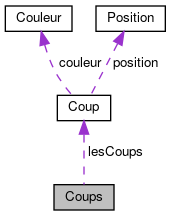
\includegraphics[width=200pt]{structCoups__coll__graph}
\end{center}
\end{figure}
\subsection*{Attributs publics}
\begin{DoxyCompactItemize}
\item 
\hyperlink{structCoup}{Coup} \hyperlink{structCoups_a97059148e0c9d3bee730b80a0f5c7982}{les\+Coups} \mbox{[}64\mbox{]}
\begin{DoxyCompactList}\small\item\em Tableau de \hyperlink{structCoup}{Coup}. \end{DoxyCompactList}\item 
\mbox{\Hypertarget{structCoups_a177e8255aeb9b85cd6ebf8e4cc64407f}\label{structCoups_a177e8255aeb9b85cd6ebf8e4cc64407f}} 
unsigned int {\bfseries nb\+Coups}
\end{DoxyCompactItemize}


\subsection{Description détaillée}
Le type \hyperlink{structCoups}{Coups} permet de stocker plusieurs \hyperlink{structCoup}{Coup}. 

Sa manipulation s\textquotesingle{}apparente à celle d\textquotesingle{}une pile L\+I\+FO. 

\subsection{Documentation des données membres}
\mbox{\Hypertarget{structCoups_a97059148e0c9d3bee730b80a0f5c7982}\label{structCoups_a97059148e0c9d3bee730b80a0f5c7982}} 
\index{Coups@{Coups}!les\+Coups@{les\+Coups}}
\index{les\+Coups@{les\+Coups}!Coups@{Coups}}
\subsubsection{\texorpdfstring{les\+Coups}{lesCoups}}
{\footnotesize\ttfamily \hyperlink{structCoup}{Coup} Coups\+::les\+Coups\mbox{[}64\mbox{]}}



Tableau de \hyperlink{structCoup}{Coup}. 



La documentation de cette structure a été générée à partir du fichier suivant \+:\begin{DoxyCompactItemize}
\item 
include/\hyperlink{Coups_8h}{Coups.\+h}\end{DoxyCompactItemize}

\hypertarget{structJoueur}{}\section{Référence de la structure Joueur}
\label{structJoueur}\index{Joueur@{Joueur}}


Le type \hyperlink{structJoueur}{Joueur} permet de manipuler une couleur en sachant si elle est jouée par une IA ou un \hyperlink{structJoueur}{Joueur} réel.  




{\ttfamily \#include $<$Joueur.\+h$>$}



Graphe de collaboration de Joueur\+:
\nopagebreak
\begin{figure}[H]
\begin{center}
\leavevmode
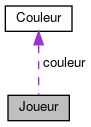
\includegraphics[width=140pt]{structJoueur__coll__graph}
\end{center}
\end{figure}
\subsection*{Attributs publics}
\begin{DoxyCompactItemize}
\item 
\mbox{\Hypertarget{structJoueur_a6abd80423308269aa3610b2e1a53f9cd}\label{structJoueur_a6abd80423308269aa3610b2e1a53f9cd}} 
int {\bfseries profondeur}
\item 
\mbox{\Hypertarget{structJoueur_a966bbda4413e0b0d7aaf109660926639}\label{structJoueur_a966bbda4413e0b0d7aaf109660926639}} 
\hyperlink{structCouleur}{Couleur} {\bfseries couleur}
\item 
\mbox{\Hypertarget{structJoueur_a229ed51bc4fd671d8657abbd26ae980f}\label{structJoueur_a229ed51bc4fd671d8657abbd26ae980f}} 
bool {\bfseries est\+IA}
\end{DoxyCompactItemize}


\subsection{Description détaillée}
Le type \hyperlink{structJoueur}{Joueur} permet de manipuler une couleur en sachant si elle est jouée par une IA ou un \hyperlink{structJoueur}{Joueur} réel. 

Cette différence influe sur la façon dont les \hyperlink{structCoup}{Coup} sont obtenus. 

La documentation de cette structure a été générée à partir du fichier suivant \+:\begin{DoxyCompactItemize}
\item 
include/\hyperlink{Joueur_8h}{Joueur.\+h}\end{DoxyCompactItemize}

\hypertarget{structPosition}{}\section{Référence de la structure Position}
\label{structPosition}\index{Position@{Position}}


Le type \hyperlink{structPosition}{Position} permet de symboliser les cases du plateau.  




{\ttfamily \#include $<$Position.\+h$>$}

\subsection*{Attributs publics}
\begin{DoxyCompactItemize}
\item 
\mbox{\Hypertarget{structPosition_aa0f9974c1f45c5384267258969f4f9b1}\label{structPosition_aa0f9974c1f45c5384267258969f4f9b1}} 
\hyperlink{Ligne_8h_a5cdc09714e36ad7319234eab8fdf5e0b}{Ligne} {\bfseries ligne}
\item 
\mbox{\Hypertarget{structPosition_af2e819310ebcffd34ae6f59cc7b33297}\label{structPosition_af2e819310ebcffd34ae6f59cc7b33297}} 
\hyperlink{Colonne_8h_aae4471c444022e1a2ce4e2af6c2d4419}{Colonne} {\bfseries colonne}
\end{DoxyCompactItemize}


\subsection{Description détaillée}
Le type \hyperlink{structPosition}{Position} permet de symboliser les cases du plateau. 

Une position est representée par une Ligne et une Colonne. 

La documentation de cette structure a été générée à partir du fichier suivant \+:\begin{DoxyCompactItemize}
\item 
include/\hyperlink{Position_8h}{Position.\+h}\end{DoxyCompactItemize}

\chapter{Documentation des fichiers}
\hypertarget{Affichage_8h}{}\section{Référence du fichier include/\+Affichage.h}
\label{Affichage_8h}\index{include/\+Affichage.\+h@{include/\+Affichage.\+h}}


Fichier contenant les fonctions d\textquotesingle{}affichage.  


{\ttfamily \#include \char`\"{}Couleur.\+h\char`\"{}}\newline
{\ttfamily \#include \char`\"{}Plateau.\+h\char`\"{}}\newline
{\ttfamily \#include \char`\"{}Joueur.\+h\char`\"{}}\newline
Graphe des dépendances par inclusion de Affichage.\+h\+:
\nopagebreak
\begin{figure}[H]
\begin{center}
\leavevmode
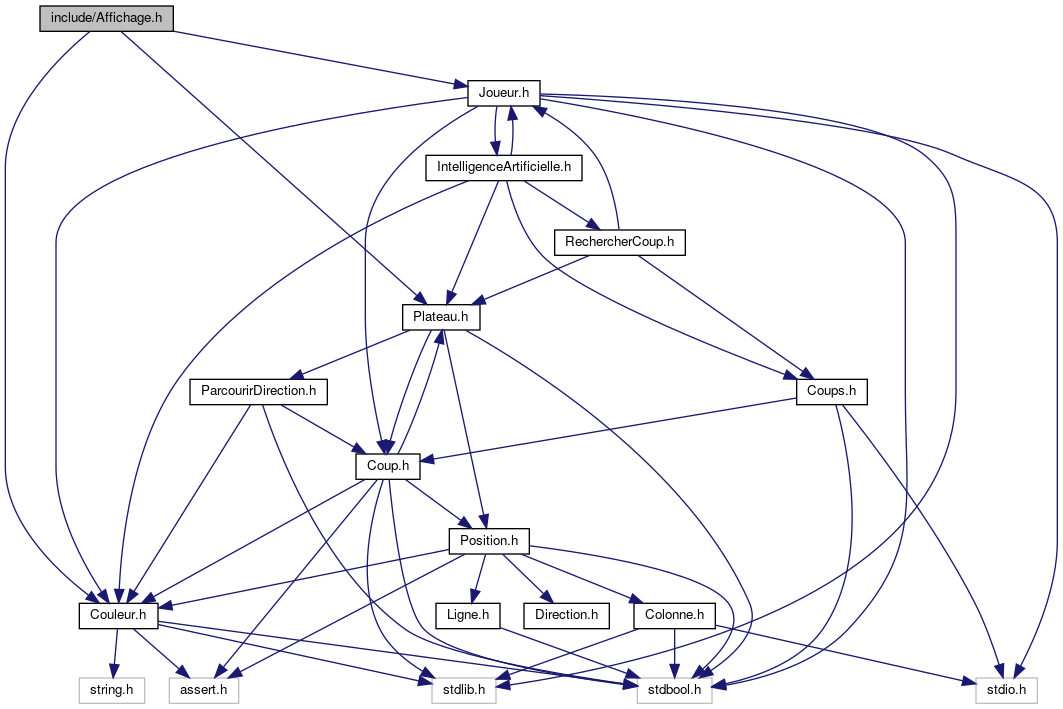
\includegraphics[width=350pt]{Affichage_8h__incl}
\end{center}
\end{figure}
Ce graphe montre quels fichiers incluent directement ou indirectement ce fichier \+:
\nopagebreak
\begin{figure}[H]
\begin{center}
\leavevmode
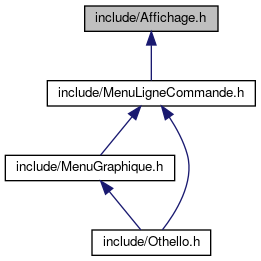
\includegraphics[width=268pt]{Affichage_8h__dep__incl}
\end{center}
\end{figure}
\subsection*{Fonctions}
\begin{DoxyCompactItemize}
\item 
void \hyperlink{Affichage_8h_a91db9073b1040dc14478d89f33e7409d}{A\+F\+F\+I\+C\+H\+A\+G\+E\+\_\+\+Afficher\+Plateau} (\hyperlink{structCouleur}{Couleur} $\ast$plateau)
\begin{DoxyCompactList}\small\item\em Affiche le plateau de jeu. \end{DoxyCompactList}\item 
void \hyperlink{Affichage_8h_af655201e2e5fff5c88686d4d6fdceca6}{A\+F\+F\+I\+C\+H\+A\+G\+E\+\_\+\+Afficher\+Plateau\+Tournois} (\hyperlink{structCouleur}{Couleur} $\ast$plateau)
\begin{DoxyCompactList}\small\item\em Affiche le plateau de jeu pour une partie en mode tournois. \end{DoxyCompactList}\item 
void \hyperlink{Affichage_8h_aca28e5d6eeae807ba3c08e8e61fd3df5}{A\+F\+F\+I\+C\+H\+A\+G\+E\+\_\+\+Afficher\+Resultats\+Partie} (\hyperlink{structCouleur}{Couleur} $\ast$plateau, \hyperlink{structJoueur}{Joueur} j1, \hyperlink{structJoueur}{Joueur} j2)
\begin{DoxyCompactList}\small\item\em Affiche les résultats de fin de partie. \end{DoxyCompactList}\item 
void \hyperlink{Affichage_8h_afc225bc9439788d4f78c7c77fdf55487}{A\+F\+F\+I\+C\+H\+A\+G\+E\+\_\+\+Afficher\+Resultats\+Partie\+Tournois} (\hyperlink{structCouleur}{Couleur} $\ast$plateau, \hyperlink{structJoueur}{Joueur} j1, \hyperlink{structJoueur}{Joueur} j2)
\begin{DoxyCompactList}\small\item\em Affiche les résultats de fin de partie en mode tournois. \end{DoxyCompactList}\item 
\mbox{\Hypertarget{Affichage_8h_af7d343da360a669c284263f6e2f2923f}\label{Affichage_8h_af7d343da360a669c284263f6e2f2923f}} 
void \hyperlink{Affichage_8h_af7d343da360a669c284263f6e2f2923f}{A\+F\+F\+I\+C\+H\+A\+G\+E\+\_\+\+Message\+Aide} ()
\begin{DoxyCompactList}\small\item\em Affiche un message d\textquotesingle{}aide concernant l\textquotesingle{}utilisation du programme et les règles du jeu. \end{DoxyCompactList}\item 
void \hyperlink{Affichage_8h_a9e25de9a63bcc359320de3b0672aec5e}{A\+F\+F\+I\+C\+H\+A\+G\+E\+\_\+\+Afficher\+Coup\+Joue} (\hyperlink{structCoup}{Coup} coup\+Joue)
\begin{DoxyCompactList}\small\item\em Affiche un \hyperlink{structCoup}{Coup} quand il est joué. \end{DoxyCompactList}\item 
void \hyperlink{Affichage_8h_ab3360912a9cd961951d655d6b3777c5c}{A\+F\+F\+I\+C\+H\+A\+G\+E\+\_\+\+Afficher\+Saisie\+Coup} (\hyperlink{structJoueur}{Joueur} joueur)
\begin{DoxyCompactList}\small\item\em Affiche une phrase pour demander la saisie d\textquotesingle{}un coup à un joueur. \end{DoxyCompactList}\item 
void \hyperlink{Affichage_8h_a168bcabce01b652ac5238fec5157b8a8}{A\+F\+F\+I\+C\+H\+A\+G\+E\+\_\+\+Afficher\+Saisie\+Coup\+Tournois} (\hyperlink{structJoueur}{Joueur} joueur)
\begin{DoxyCompactList}\small\item\em Affiche une phrase pour demander la saisie d\textquotesingle{}un coup à un joueur. \end{DoxyCompactList}\end{DoxyCompactItemize}


\subsection{Description détaillée}
Fichier contenant les fonctions d\textquotesingle{}affichage. 



\subsection{Documentation des fonctions}
\mbox{\Hypertarget{Affichage_8h_a9e25de9a63bcc359320de3b0672aec5e}\label{Affichage_8h_a9e25de9a63bcc359320de3b0672aec5e}} 
\index{Affichage.\+h@{Affichage.\+h}!A\+F\+F\+I\+C\+H\+A\+G\+E\+\_\+\+Afficher\+Coup\+Joue@{A\+F\+F\+I\+C\+H\+A\+G\+E\+\_\+\+Afficher\+Coup\+Joue}}
\index{A\+F\+F\+I\+C\+H\+A\+G\+E\+\_\+\+Afficher\+Coup\+Joue@{A\+F\+F\+I\+C\+H\+A\+G\+E\+\_\+\+Afficher\+Coup\+Joue}!Affichage.\+h@{Affichage.\+h}}
\subsubsection{\texorpdfstring{A\+F\+F\+I\+C\+H\+A\+G\+E\+\_\+\+Afficher\+Coup\+Joue()}{AFFICHAGE\_AfficherCoupJoue()}}
{\footnotesize\ttfamily void A\+F\+F\+I\+C\+H\+A\+G\+E\+\_\+\+Afficher\+Coup\+Joue (\begin{DoxyParamCaption}\item[{\hyperlink{structCoup}{Coup}}]{coup\+Joue }\end{DoxyParamCaption})}



Affiche un \hyperlink{structCoup}{Coup} quand il est joué. 

Utile nottament pour envoyer le \hyperlink{structCoup}{Coup} sur la sortie standard en mode tournois.


\begin{DoxyParams}{Paramètres}
{\em coup\+Joue} & \hyperlink{structCoup}{Coup} qui doit être affiché \\
\hline
\end{DoxyParams}
\mbox{\Hypertarget{Affichage_8h_a91db9073b1040dc14478d89f33e7409d}\label{Affichage_8h_a91db9073b1040dc14478d89f33e7409d}} 
\index{Affichage.\+h@{Affichage.\+h}!A\+F\+F\+I\+C\+H\+A\+G\+E\+\_\+\+Afficher\+Plateau@{A\+F\+F\+I\+C\+H\+A\+G\+E\+\_\+\+Afficher\+Plateau}}
\index{A\+F\+F\+I\+C\+H\+A\+G\+E\+\_\+\+Afficher\+Plateau@{A\+F\+F\+I\+C\+H\+A\+G\+E\+\_\+\+Afficher\+Plateau}!Affichage.\+h@{Affichage.\+h}}
\subsubsection{\texorpdfstring{A\+F\+F\+I\+C\+H\+A\+G\+E\+\_\+\+Afficher\+Plateau()}{AFFICHAGE\_AfficherPlateau()}}
{\footnotesize\ttfamily void A\+F\+F\+I\+C\+H\+A\+G\+E\+\_\+\+Afficher\+Plateau (\begin{DoxyParamCaption}\item[{\hyperlink{structCouleur}{Couleur} $\ast$}]{plateau }\end{DoxyParamCaption})}



Affiche le plateau de jeu. 

Le plateau est affiché sur la sortie standard (terminal). Les lettres du dessus correspondent aux colonnes du jeu et les chiffres sur le côté sont les lignes. A l\textquotesingle{}intersection d\textquotesingle{}une ligne et d\textquotesingle{}une colonne se trouve un symbole significatif de la couleur présente sur la case.


\begin{DoxyParams}{Paramètres}
{\em plateau} & Plateau de jeu. \\
\hline
\end{DoxyParams}
\mbox{\Hypertarget{Affichage_8h_af655201e2e5fff5c88686d4d6fdceca6}\label{Affichage_8h_af655201e2e5fff5c88686d4d6fdceca6}} 
\index{Affichage.\+h@{Affichage.\+h}!A\+F\+F\+I\+C\+H\+A\+G\+E\+\_\+\+Afficher\+Plateau\+Tournois@{A\+F\+F\+I\+C\+H\+A\+G\+E\+\_\+\+Afficher\+Plateau\+Tournois}}
\index{A\+F\+F\+I\+C\+H\+A\+G\+E\+\_\+\+Afficher\+Plateau\+Tournois@{A\+F\+F\+I\+C\+H\+A\+G\+E\+\_\+\+Afficher\+Plateau\+Tournois}!Affichage.\+h@{Affichage.\+h}}
\subsubsection{\texorpdfstring{A\+F\+F\+I\+C\+H\+A\+G\+E\+\_\+\+Afficher\+Plateau\+Tournois()}{AFFICHAGE\_AfficherPlateauTournois()}}
{\footnotesize\ttfamily void A\+F\+F\+I\+C\+H\+A\+G\+E\+\_\+\+Afficher\+Plateau\+Tournois (\begin{DoxyParamCaption}\item[{\hyperlink{structCouleur}{Couleur} $\ast$}]{plateau }\end{DoxyParamCaption})}



Affiche le plateau de jeu pour une partie en mode tournois. 

Pour l\textquotesingle{}instant il n\textquotesingle{}est pas nécessaire d\textquotesingle{}afficher le plateau quand la partie est jouée en mode tournois, donc la fonction n\textquotesingle{}affiche rien.


\begin{DoxyParams}{Paramètres}
{\em plateau} & Plateau de jeu. \\
\hline
\end{DoxyParams}
\mbox{\Hypertarget{Affichage_8h_aca28e5d6eeae807ba3c08e8e61fd3df5}\label{Affichage_8h_aca28e5d6eeae807ba3c08e8e61fd3df5}} 
\index{Affichage.\+h@{Affichage.\+h}!A\+F\+F\+I\+C\+H\+A\+G\+E\+\_\+\+Afficher\+Resultats\+Partie@{A\+F\+F\+I\+C\+H\+A\+G\+E\+\_\+\+Afficher\+Resultats\+Partie}}
\index{A\+F\+F\+I\+C\+H\+A\+G\+E\+\_\+\+Afficher\+Resultats\+Partie@{A\+F\+F\+I\+C\+H\+A\+G\+E\+\_\+\+Afficher\+Resultats\+Partie}!Affichage.\+h@{Affichage.\+h}}
\subsubsection{\texorpdfstring{A\+F\+F\+I\+C\+H\+A\+G\+E\+\_\+\+Afficher\+Resultats\+Partie()}{AFFICHAGE\_AfficherResultatsPartie()}}
{\footnotesize\ttfamily void A\+F\+F\+I\+C\+H\+A\+G\+E\+\_\+\+Afficher\+Resultats\+Partie (\begin{DoxyParamCaption}\item[{\hyperlink{structCouleur}{Couleur} $\ast$}]{plateau,  }\item[{\hyperlink{structJoueur}{Joueur}}]{j1,  }\item[{\hyperlink{structJoueur}{Joueur}}]{j2 }\end{DoxyParamCaption})}



Affiche les résultats de fin de partie. 

Affiche le score total de chaque joueur ( c\textquotesingle{}est à dire le nombre de cases portant sa couleur présentes sur le plateau ) ainsi que le vainqueur de la partie. Affiche égalité en cas d\textquotesingle{}égalité.


\begin{DoxyParams}{Paramètres}
{\em plateau} & Plateau de jeu. \\
\hline
\end{DoxyParams}
\mbox{\Hypertarget{Affichage_8h_afc225bc9439788d4f78c7c77fdf55487}\label{Affichage_8h_afc225bc9439788d4f78c7c77fdf55487}} 
\index{Affichage.\+h@{Affichage.\+h}!A\+F\+F\+I\+C\+H\+A\+G\+E\+\_\+\+Afficher\+Resultats\+Partie\+Tournois@{A\+F\+F\+I\+C\+H\+A\+G\+E\+\_\+\+Afficher\+Resultats\+Partie\+Tournois}}
\index{A\+F\+F\+I\+C\+H\+A\+G\+E\+\_\+\+Afficher\+Resultats\+Partie\+Tournois@{A\+F\+F\+I\+C\+H\+A\+G\+E\+\_\+\+Afficher\+Resultats\+Partie\+Tournois}!Affichage.\+h@{Affichage.\+h}}
\subsubsection{\texorpdfstring{A\+F\+F\+I\+C\+H\+A\+G\+E\+\_\+\+Afficher\+Resultats\+Partie\+Tournois()}{AFFICHAGE\_AfficherResultatsPartieTournois()}}
{\footnotesize\ttfamily void A\+F\+F\+I\+C\+H\+A\+G\+E\+\_\+\+Afficher\+Resultats\+Partie\+Tournois (\begin{DoxyParamCaption}\item[{\hyperlink{structCouleur}{Couleur} $\ast$}]{plateau,  }\item[{\hyperlink{structJoueur}{Joueur}}]{j1,  }\item[{\hyperlink{structJoueur}{Joueur}}]{j2 }\end{DoxyParamCaption})}



Affiche les résultats de fin de partie en mode tournois. 

Pour l\textquotesingle{}instant il n\textquotesingle{}est pas nécessaire d\textquotesingle{}afficher les résultats quand la partie est en mode tournois, donc la fonction n\textquotesingle{}affiche rien.


\begin{DoxyParams}{Paramètres}
{\em plateau} & Plateau de jeu \\
\hline
\end{DoxyParams}
\mbox{\Hypertarget{Affichage_8h_ab3360912a9cd961951d655d6b3777c5c}\label{Affichage_8h_ab3360912a9cd961951d655d6b3777c5c}} 
\index{Affichage.\+h@{Affichage.\+h}!A\+F\+F\+I\+C\+H\+A\+G\+E\+\_\+\+Afficher\+Saisie\+Coup@{A\+F\+F\+I\+C\+H\+A\+G\+E\+\_\+\+Afficher\+Saisie\+Coup}}
\index{A\+F\+F\+I\+C\+H\+A\+G\+E\+\_\+\+Afficher\+Saisie\+Coup@{A\+F\+F\+I\+C\+H\+A\+G\+E\+\_\+\+Afficher\+Saisie\+Coup}!Affichage.\+h@{Affichage.\+h}}
\subsubsection{\texorpdfstring{A\+F\+F\+I\+C\+H\+A\+G\+E\+\_\+\+Afficher\+Saisie\+Coup()}{AFFICHAGE\_AfficherSaisieCoup()}}
{\footnotesize\ttfamily void A\+F\+F\+I\+C\+H\+A\+G\+E\+\_\+\+Afficher\+Saisie\+Coup (\begin{DoxyParamCaption}\item[{\hyperlink{structJoueur}{Joueur}}]{joueur }\end{DoxyParamCaption})}



Affiche une phrase pour demander la saisie d\textquotesingle{}un coup à un joueur. 


\begin{DoxyParams}{Paramètres}
{\em joueur} & \hyperlink{structJoueur}{Joueur} qui doit saisir son coup. \\
\hline
\end{DoxyParams}
\mbox{\Hypertarget{Affichage_8h_a168bcabce01b652ac5238fec5157b8a8}\label{Affichage_8h_a168bcabce01b652ac5238fec5157b8a8}} 
\index{Affichage.\+h@{Affichage.\+h}!A\+F\+F\+I\+C\+H\+A\+G\+E\+\_\+\+Afficher\+Saisie\+Coup\+Tournois@{A\+F\+F\+I\+C\+H\+A\+G\+E\+\_\+\+Afficher\+Saisie\+Coup\+Tournois}}
\index{A\+F\+F\+I\+C\+H\+A\+G\+E\+\_\+\+Afficher\+Saisie\+Coup\+Tournois@{A\+F\+F\+I\+C\+H\+A\+G\+E\+\_\+\+Afficher\+Saisie\+Coup\+Tournois}!Affichage.\+h@{Affichage.\+h}}
\subsubsection{\texorpdfstring{A\+F\+F\+I\+C\+H\+A\+G\+E\+\_\+\+Afficher\+Saisie\+Coup\+Tournois()}{AFFICHAGE\_AfficherSaisieCoupTournois()}}
{\footnotesize\ttfamily void A\+F\+F\+I\+C\+H\+A\+G\+E\+\_\+\+Afficher\+Saisie\+Coup\+Tournois (\begin{DoxyParamCaption}\item[{\hyperlink{structJoueur}{Joueur}}]{joueur }\end{DoxyParamCaption})}



Affiche une phrase pour demander la saisie d\textquotesingle{}un coup à un joueur. 

Pour l\textquotesingle{}instant en mode tournoi aucun affichage n\textquotesingle{}est demandé, voir même cela peut entraver le bon fonctionnement si des printf sont utilisés.


\begin{DoxyParams}{Paramètres}
{\em joueur} & \hyperlink{structJoueur}{Joueur} qui doit saisir son coup. \\
\hline
\end{DoxyParams}

\hypertarget{Colonne_8h}{}\section{Référence du fichier include/\+Colonne.h}
\label{Colonne_8h}\index{include/\+Colonne.\+h@{include/\+Colonne.\+h}}


Fichier contenant la définition de l\textquotesingle{}enum Colonne et de ses fonctions associées.  


{\ttfamily \#include $<$stdbool.\+h$>$}\newline
{\ttfamily \#include $<$stdlib.\+h$>$}\newline
{\ttfamily \#include $<$stdio.\+h$>$}\newline
Graphe des dépendances par inclusion de Colonne.\+h\+:
\nopagebreak
\begin{figure}[H]
\begin{center}
\leavevmode
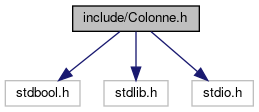
\includegraphics[width=266pt]{Colonne_8h__incl}
\end{center}
\end{figure}
Ce graphe montre quels fichiers incluent directement ou indirectement ce fichier \+:
\nopagebreak
\begin{figure}[H]
\begin{center}
\leavevmode
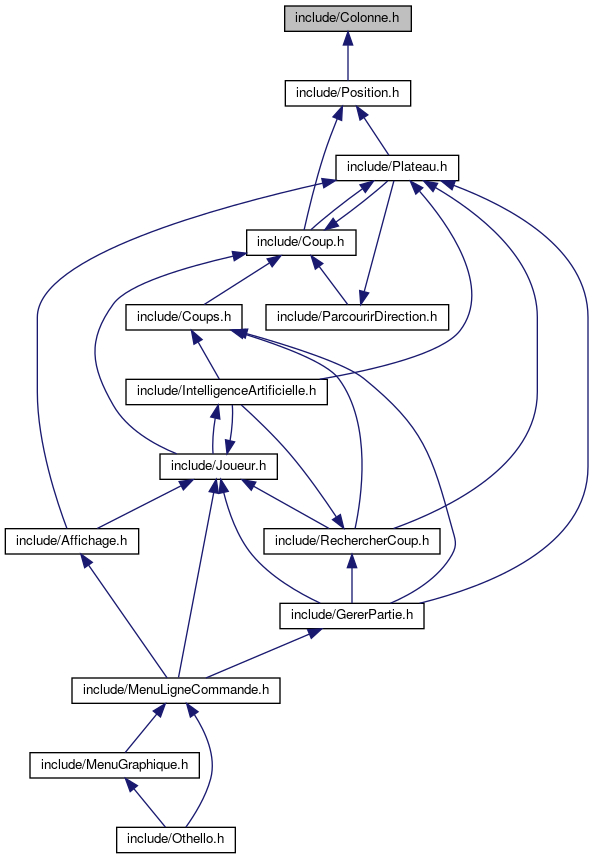
\includegraphics[width=350pt]{Colonne_8h__dep__incl}
\end{center}
\end{figure}
\subsection*{Macros}
\begin{DoxyCompactItemize}
\item 
\mbox{\Hypertarget{Colonne_8h_ab336b9c20ef5ab377a509ed2a868fc06}\label{Colonne_8h_ab336b9c20ef5ab377a509ed2a868fc06}} 
\#define {\bfseries K\+E\+Y\+\_\+\+E\+R\+R\+OR}~1;
\end{DoxyCompactItemize}
\subsection*{Énumérations}
\begin{DoxyCompactItemize}
\item 
\mbox{\Hypertarget{Colonne_8h_aae4471c444022e1a2ce4e2af6c2d4419}\label{Colonne_8h_aae4471c444022e1a2ce4e2af6c2d4419}} 
enum \hyperlink{Colonne_8h_aae4471c444022e1a2ce4e2af6c2d4419}{Colonne} \{ \newline
{\bfseries a}, 
{\bfseries b}, 
{\bfseries c}, 
{\bfseries d}, 
\newline
{\bfseries e}, 
{\bfseries f}, 
{\bfseries g}, 
{\bfseries h}
 \}\begin{DoxyCompactList}\small\item\em L\textquotesingle{}énumeration permet de travailler avec les Colonne comme des caractères. \end{DoxyCompactList}
\end{DoxyCompactItemize}
\subsection*{Fonctions}
\begin{DoxyCompactItemize}
\item 
\mbox{\Hypertarget{Colonne_8h_ab065dc846199785e818e58193166b225}\label{Colonne_8h_ab065dc846199785e818e58193166b225}} 
\hyperlink{Colonne_8h_aae4471c444022e1a2ce4e2af6c2d4419}{Colonne} {\bfseries C\+O\+L\+O\+N\+N\+E\+\_\+\+Obtenir\+Colonne\+Depuis\+Int} (int col\+Num)
\item 
\mbox{\Hypertarget{Colonne_8h_ae121cda9a79f4a1c0b4588d6fc86fb0a}\label{Colonne_8h_ae121cda9a79f4a1c0b4588d6fc86fb0a}} 
\hyperlink{Colonne_8h_aae4471c444022e1a2ce4e2af6c2d4419}{Colonne} {\bfseries C\+O\+L\+O\+N\+N\+E\+\_\+\+Obtenir\+Colonne\+Depuis\+Char} (char col\+Char)
\item 
\mbox{\Hypertarget{Colonne_8h_a2b02bdf3f1facdc3c15a9e1d373f7b71}\label{Colonne_8h_a2b02bdf3f1facdc3c15a9e1d373f7b71}} 
char {\bfseries C\+O\+L\+O\+N\+N\+E\+\_\+\+Obtenir\+Char\+Depuis\+Colonne} (\hyperlink{Colonne_8h_aae4471c444022e1a2ce4e2af6c2d4419}{Colonne} c)
\item 
\mbox{\Hypertarget{Colonne_8h_ac7ab884c3695241f08d1d936258fd156}\label{Colonne_8h_ac7ab884c3695241f08d1d936258fd156}} 
int {\bfseries C\+O\+L\+O\+N\+N\+E\+\_\+\+Obtenir\+Numero\+Colonne} (\hyperlink{Colonne_8h_aae4471c444022e1a2ce4e2af6c2d4419}{Colonne} colonne)
\item 
bool \hyperlink{Colonne_8h_a3fc6d37121048692933477793b92fab7}{C\+O\+L\+O\+N\+N\+E\+\_\+\+Sont\+Egales\+Colonnes} (\hyperlink{Colonne_8h_aae4471c444022e1a2ce4e2af6c2d4419}{Colonne} colonne1, \hyperlink{Colonne_8h_aae4471c444022e1a2ce4e2af6c2d4419}{Colonne} colonne2)
\begin{DoxyCompactList}\small\item\em Détermine si deux Colonne sont égales. \end{DoxyCompactList}\end{DoxyCompactItemize}


\subsection{Description détaillée}
Fichier contenant la définition de l\textquotesingle{}enum Colonne et de ses fonctions associées. 



\subsection{Documentation des fonctions}
\mbox{\Hypertarget{Colonne_8h_a3fc6d37121048692933477793b92fab7}\label{Colonne_8h_a3fc6d37121048692933477793b92fab7}} 
\index{Colonne.\+h@{Colonne.\+h}!C\+O\+L\+O\+N\+N\+E\+\_\+\+Sont\+Egales\+Colonnes@{C\+O\+L\+O\+N\+N\+E\+\_\+\+Sont\+Egales\+Colonnes}}
\index{C\+O\+L\+O\+N\+N\+E\+\_\+\+Sont\+Egales\+Colonnes@{C\+O\+L\+O\+N\+N\+E\+\_\+\+Sont\+Egales\+Colonnes}!Colonne.\+h@{Colonne.\+h}}
\subsubsection{\texorpdfstring{C\+O\+L\+O\+N\+N\+E\+\_\+\+Sont\+Egales\+Colonnes()}{COLONNE\_SontEgalesColonnes()}}
{\footnotesize\ttfamily bool C\+O\+L\+O\+N\+N\+E\+\_\+\+Sont\+Egales\+Colonnes (\begin{DoxyParamCaption}\item[{\hyperlink{Colonne_8h_aae4471c444022e1a2ce4e2af6c2d4419}{Colonne}}]{colonne1,  }\item[{\hyperlink{Colonne_8h_aae4471c444022e1a2ce4e2af6c2d4419}{Colonne}}]{colonne2 }\end{DoxyParamCaption})}



Détermine si deux Colonne sont égales. 


\begin{DoxyParams}{Paramètres}
{\em colonne1} & Première Colonne à comparer. \\
\hline
{\em colonne2} & Deuxième Colonne à comparer.\\
\hline
\end{DoxyParams}
\begin{DoxyReturn}{Renvoie}
true si les Colonne sont égales, false sinon. 
\end{DoxyReturn}

\hypertarget{Couleur_8h}{}\section{Référence du fichier include/\+Couleur.h}
\label{Couleur_8h}\index{include/\+Couleur.\+h@{include/\+Couleur.\+h}}


Fichier contenant la définition du type \hyperlink{structCouleur}{Couleur}, l\textquotesingle{}enum nom\+Couleur et de leurs fonctions associées.  


{\ttfamily \#include $<$stdbool.\+h$>$}\newline
{\ttfamily \#include $<$string.\+h$>$}\newline
{\ttfamily \#include $<$stdlib.\+h$>$}\newline
{\ttfamily \#include $<$assert.\+h$>$}\newline
Graphe des dépendances par inclusion de Couleur.\+h\+:
\nopagebreak
\begin{figure}[H]
\begin{center}
\leavevmode
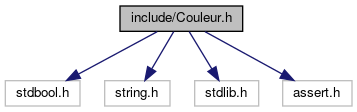
\includegraphics[width=340pt]{Couleur_8h__incl}
\end{center}
\end{figure}
Ce graphe montre quels fichiers incluent directement ou indirectement ce fichier \+:
\nopagebreak
\begin{figure}[H]
\begin{center}
\leavevmode
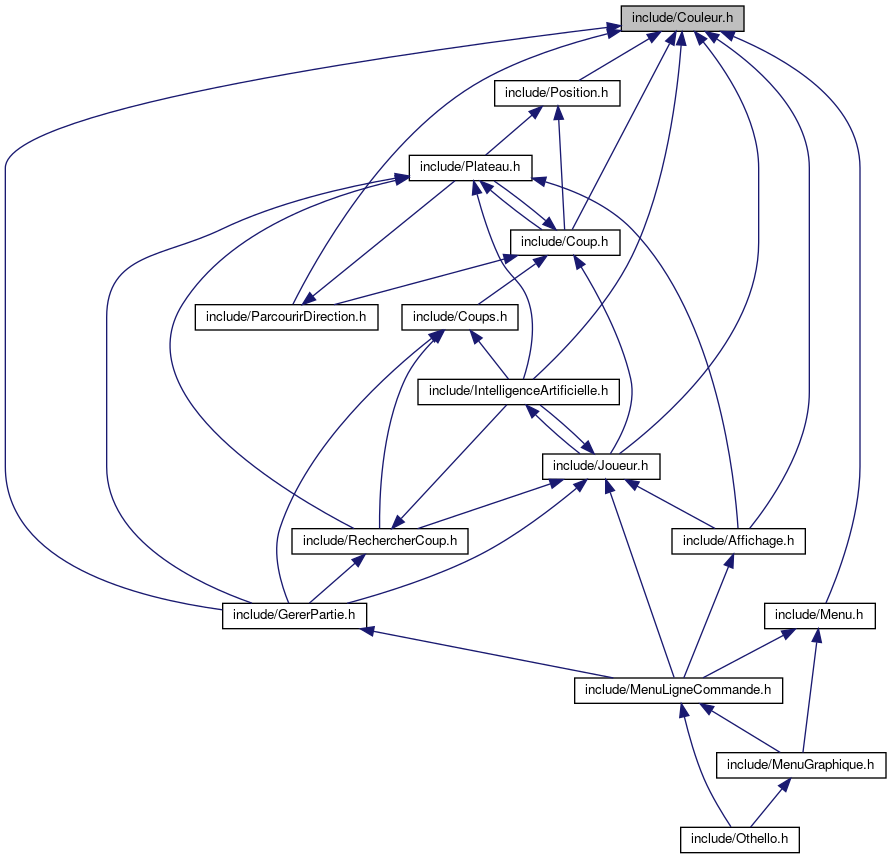
\includegraphics[width=350pt]{Couleur_8h__dep__incl}
\end{center}
\end{figure}
\subsection*{Classes}
\begin{DoxyCompactItemize}
\item 
struct \hyperlink{structCouleur}{Couleur}
\begin{DoxyCompactList}\small\item\em Le type \hyperlink{structCouleur}{Couleur} permet de symboliser un pion. \end{DoxyCompactList}\end{DoxyCompactItemize}
\subsection*{Macros}
\begin{DoxyCompactItemize}
\item 
\mbox{\Hypertarget{Couleur_8h_a844c90632f9b272c048c8f800ae98461}\label{Couleur_8h_a844c90632f9b272c048c8f800ae98461}} 
\#define {\bfseries C\+O\+U\+L\+E\+U\+R\+\_\+\+B\+L\+A\+N\+C\+HE}~\char`\"{}blanc\char`\"{}
\item 
\mbox{\Hypertarget{Couleur_8h_a795d6ee681a219152414e14af5de8c6a}\label{Couleur_8h_a795d6ee681a219152414e14af5de8c6a}} 
\#define {\bfseries C\+O\+U\+L\+E\+U\+R\+\_\+\+N\+O\+I\+RE}~\char`\"{}noir\char`\"{}
\item 
\mbox{\Hypertarget{Couleur_8h_abc41d785889c9cf253cdd2702735fc54}\label{Couleur_8h_abc41d785889c9cf253cdd2702735fc54}} 
\#define {\bfseries C\+O\+U\+L\+E\+U\+R\+\_\+\+N\+E\+U\+T\+RE}~\char`\"{}neutre\char`\"{}
\end{DoxyCompactItemize}
\subsection*{Énumérations}
\begin{DoxyCompactItemize}
\item 
\mbox{\Hypertarget{Couleur_8h_aaca4e6192fa64673e34ef06ceb76bb16}\label{Couleur_8h_aaca4e6192fa64673e34ef06ceb76bb16}} 
enum \hyperlink{Couleur_8h_aaca4e6192fa64673e34ef06ceb76bb16}{nom\+Couleur} \{ {\bfseries Neutre}, 
{\bfseries Blanc}, 
{\bfseries Noir}
 \}\begin{DoxyCompactList}\small\item\em L\textquotesingle{}énumeration nom\+Couleur permet de définir un ensemble de valeurs possibles pour le nom des couleurs. \end{DoxyCompactList}
\end{DoxyCompactItemize}
\subsection*{Fonctions}
\begin{DoxyCompactItemize}
\item 
\hyperlink{structCouleur}{Couleur} \hyperlink{Couleur_8h_abe9e2c9e1f3de354428e39e43c6a3c24}{C\+O\+U\+L\+E\+U\+R\+\_\+\+Obtenir\+Couleur\+Noir} ()
\begin{DoxyCompactList}\small\item\em Crée une \hyperlink{structCouleur}{Couleur} noire. \end{DoxyCompactList}\item 
\hyperlink{structCouleur}{Couleur} \hyperlink{Couleur_8h_a46a2c4b27022ac80b7d073790e8bfcda}{C\+O\+U\+L\+E\+U\+R\+\_\+\+Obtenir\+Couleur\+Blanc} ()
\begin{DoxyCompactList}\small\item\em Crée une \hyperlink{structCouleur}{Couleur} blanche. \end{DoxyCompactList}\item 
\hyperlink{structCouleur}{Couleur} \hyperlink{Couleur_8h_aed24736ec4b229943d1d1f67439f438c}{C\+O\+U\+L\+E\+U\+R\+\_\+\+Obtenir\+Couleur\+Neutre} ()
\begin{DoxyCompactList}\small\item\em Crée une \hyperlink{structCouleur}{Couleur} neutre. \end{DoxyCompactList}\item 
\mbox{\Hypertarget{Couleur_8h_a6aef9afb2c70e99dad27150a530891d6}\label{Couleur_8h_a6aef9afb2c70e99dad27150a530891d6}} 
\hyperlink{structCouleur}{Couleur} {\bfseries C\+O\+U\+L\+E\+U\+R\+\_\+\+Obtenir\+Couleur\+Opposee} (\hyperlink{structCouleur}{Couleur} couleur)
\item 
bool \hyperlink{Couleur_8h_a65508cd85f4651b72b8120e3173b145b}{C\+O\+U\+L\+E\+U\+R\+\_\+\+Est\+Neutre} (\hyperlink{structCouleur}{Couleur} couleur)
\begin{DoxyCompactList}\small\item\em Détermine si la \hyperlink{structCouleur}{Couleur} passée en entrée est une couleur neutre. \end{DoxyCompactList}\item 
bool \hyperlink{Couleur_8h_a2f818000b78b17149b8b63d1191c153b}{C\+O\+U\+L\+E\+U\+R\+\_\+\+Sont\+Egales\+Couleurs} (\hyperlink{structCouleur}{Couleur} couleur1, \hyperlink{structCouleur}{Couleur} couleur2)
\begin{DoxyCompactList}\small\item\em Détermine si les \hyperlink{structCouleur}{Couleur} sont identiques. \end{DoxyCompactList}\item 
\hyperlink{structCouleur}{Couleur} \hyperlink{Couleur_8h_a4c53c074b7757521f7228ed215e87e3a}{C\+O\+U\+L\+E\+U\+R\+\_\+\+Obtenir\+Couleur\+Depuis\+String} (char $\ast$couleur)
\begin{DoxyCompactList}\small\item\em Obtient une instance de \hyperlink{structCouleur}{Couleur} grâce à un String indiquant son nom. \end{DoxyCompactList}\item 
char $\ast$ \hyperlink{Couleur_8h_ad0dad7182393f92a0831661263c63e4c}{C\+O\+U\+L\+E\+U\+R\+\_\+\+Obtenir\+Str} (\hyperlink{structCouleur}{Couleur} couleur)
\begin{DoxyCompactList}\small\item\em Permet de retourner la chaine de caractères correspondante à une couleur. \end{DoxyCompactList}\item 
char \hyperlink{Couleur_8h_a36de4a580e681c96e8641327b2b1ed41}{C\+O\+U\+L\+E\+U\+R\+\_\+\+Obtenir\+Symbole} (\hyperlink{structCouleur}{Couleur} couleur)
\begin{DoxyCompactList}\small\item\em Permet d\textquotesingle{}accéder au champs symbole d\textquotesingle{}une instance de \hyperlink{structCouleur}{Couleur}. \end{DoxyCompactList}\end{DoxyCompactItemize}


\subsection{Description détaillée}
Fichier contenant la définition du type \hyperlink{structCouleur}{Couleur}, l\textquotesingle{}enum nom\+Couleur et de leurs fonctions associées. 



\subsection{Documentation des fonctions}
\mbox{\Hypertarget{Couleur_8h_a65508cd85f4651b72b8120e3173b145b}\label{Couleur_8h_a65508cd85f4651b72b8120e3173b145b}} 
\index{Couleur.\+h@{Couleur.\+h}!C\+O\+U\+L\+E\+U\+R\+\_\+\+Est\+Neutre@{C\+O\+U\+L\+E\+U\+R\+\_\+\+Est\+Neutre}}
\index{C\+O\+U\+L\+E\+U\+R\+\_\+\+Est\+Neutre@{C\+O\+U\+L\+E\+U\+R\+\_\+\+Est\+Neutre}!Couleur.\+h@{Couleur.\+h}}
\subsubsection{\texorpdfstring{C\+O\+U\+L\+E\+U\+R\+\_\+\+Est\+Neutre()}{COULEUR\_EstNeutre()}}
{\footnotesize\ttfamily bool C\+O\+U\+L\+E\+U\+R\+\_\+\+Est\+Neutre (\begin{DoxyParamCaption}\item[{\hyperlink{structCouleur}{Couleur}}]{couleur }\end{DoxyParamCaption})}



Détermine si la \hyperlink{structCouleur}{Couleur} passée en entrée est une couleur neutre. 


\begin{DoxyParams}{Paramètres}
{\em couleur} & \hyperlink{structCouleur}{Couleur} dont on souhaite vérifier la neutralité.\\
\hline
\end{DoxyParams}
\begin{DoxyReturn}{Renvoie}
true si la \hyperlink{structCouleur}{Couleur} est neutre, false sinon. 
\end{DoxyReturn}
\mbox{\Hypertarget{Couleur_8h_a46a2c4b27022ac80b7d073790e8bfcda}\label{Couleur_8h_a46a2c4b27022ac80b7d073790e8bfcda}} 
\index{Couleur.\+h@{Couleur.\+h}!C\+O\+U\+L\+E\+U\+R\+\_\+\+Obtenir\+Couleur\+Blanc@{C\+O\+U\+L\+E\+U\+R\+\_\+\+Obtenir\+Couleur\+Blanc}}
\index{C\+O\+U\+L\+E\+U\+R\+\_\+\+Obtenir\+Couleur\+Blanc@{C\+O\+U\+L\+E\+U\+R\+\_\+\+Obtenir\+Couleur\+Blanc}!Couleur.\+h@{Couleur.\+h}}
\subsubsection{\texorpdfstring{C\+O\+U\+L\+E\+U\+R\+\_\+\+Obtenir\+Couleur\+Blanc()}{COULEUR\_ObtenirCouleurBlanc()}}
{\footnotesize\ttfamily \hyperlink{structCouleur}{Couleur} C\+O\+U\+L\+E\+U\+R\+\_\+\+Obtenir\+Couleur\+Blanc (\begin{DoxyParamCaption}{ }\end{DoxyParamCaption})}



Crée une \hyperlink{structCouleur}{Couleur} blanche. 

\begin{DoxyReturn}{Renvoie}
Instance de \hyperlink{structCouleur}{Couleur} blanche. 
\end{DoxyReturn}
\mbox{\Hypertarget{Couleur_8h_a4c53c074b7757521f7228ed215e87e3a}\label{Couleur_8h_a4c53c074b7757521f7228ed215e87e3a}} 
\index{Couleur.\+h@{Couleur.\+h}!C\+O\+U\+L\+E\+U\+R\+\_\+\+Obtenir\+Couleur\+Depuis\+String@{C\+O\+U\+L\+E\+U\+R\+\_\+\+Obtenir\+Couleur\+Depuis\+String}}
\index{C\+O\+U\+L\+E\+U\+R\+\_\+\+Obtenir\+Couleur\+Depuis\+String@{C\+O\+U\+L\+E\+U\+R\+\_\+\+Obtenir\+Couleur\+Depuis\+String}!Couleur.\+h@{Couleur.\+h}}
\subsubsection{\texorpdfstring{C\+O\+U\+L\+E\+U\+R\+\_\+\+Obtenir\+Couleur\+Depuis\+String()}{COULEUR\_ObtenirCouleurDepuisString()}}
{\footnotesize\ttfamily \hyperlink{structCouleur}{Couleur} C\+O\+U\+L\+E\+U\+R\+\_\+\+Obtenir\+Couleur\+Depuis\+String (\begin{DoxyParamCaption}\item[{char $\ast$}]{couleur }\end{DoxyParamCaption})}



Obtient une instance de \hyperlink{structCouleur}{Couleur} grâce à un String indiquant son nom. 


\begin{DoxyParams}{Paramètres}
{\em couleur} & String correspondant au nom de la couleur que l\textquotesingle{}on souhaite obtenir.\\
\hline
\end{DoxyParams}
\begin{DoxyReturn}{Renvoie}
Instance de couleur. 
\end{DoxyReturn}
\mbox{\Hypertarget{Couleur_8h_aed24736ec4b229943d1d1f67439f438c}\label{Couleur_8h_aed24736ec4b229943d1d1f67439f438c}} 
\index{Couleur.\+h@{Couleur.\+h}!C\+O\+U\+L\+E\+U\+R\+\_\+\+Obtenir\+Couleur\+Neutre@{C\+O\+U\+L\+E\+U\+R\+\_\+\+Obtenir\+Couleur\+Neutre}}
\index{C\+O\+U\+L\+E\+U\+R\+\_\+\+Obtenir\+Couleur\+Neutre@{C\+O\+U\+L\+E\+U\+R\+\_\+\+Obtenir\+Couleur\+Neutre}!Couleur.\+h@{Couleur.\+h}}
\subsubsection{\texorpdfstring{C\+O\+U\+L\+E\+U\+R\+\_\+\+Obtenir\+Couleur\+Neutre()}{COULEUR\_ObtenirCouleurNeutre()}}
{\footnotesize\ttfamily \hyperlink{structCouleur}{Couleur} C\+O\+U\+L\+E\+U\+R\+\_\+\+Obtenir\+Couleur\+Neutre (\begin{DoxyParamCaption}{ }\end{DoxyParamCaption})}



Crée une \hyperlink{structCouleur}{Couleur} neutre. 

\begin{DoxyReturn}{Renvoie}
Instance de \hyperlink{structCouleur}{Couleur} neutre. 
\end{DoxyReturn}
\mbox{\Hypertarget{Couleur_8h_abe9e2c9e1f3de354428e39e43c6a3c24}\label{Couleur_8h_abe9e2c9e1f3de354428e39e43c6a3c24}} 
\index{Couleur.\+h@{Couleur.\+h}!C\+O\+U\+L\+E\+U\+R\+\_\+\+Obtenir\+Couleur\+Noir@{C\+O\+U\+L\+E\+U\+R\+\_\+\+Obtenir\+Couleur\+Noir}}
\index{C\+O\+U\+L\+E\+U\+R\+\_\+\+Obtenir\+Couleur\+Noir@{C\+O\+U\+L\+E\+U\+R\+\_\+\+Obtenir\+Couleur\+Noir}!Couleur.\+h@{Couleur.\+h}}
\subsubsection{\texorpdfstring{C\+O\+U\+L\+E\+U\+R\+\_\+\+Obtenir\+Couleur\+Noir()}{COULEUR\_ObtenirCouleurNoir()}}
{\footnotesize\ttfamily \hyperlink{structCouleur}{Couleur} C\+O\+U\+L\+E\+U\+R\+\_\+\+Obtenir\+Couleur\+Noir (\begin{DoxyParamCaption}{ }\end{DoxyParamCaption})}



Crée une \hyperlink{structCouleur}{Couleur} noire. 

\begin{DoxyReturn}{Renvoie}
Instance de \hyperlink{structCouleur}{Couleur} noire. 
\end{DoxyReturn}
\mbox{\Hypertarget{Couleur_8h_ad0dad7182393f92a0831661263c63e4c}\label{Couleur_8h_ad0dad7182393f92a0831661263c63e4c}} 
\index{Couleur.\+h@{Couleur.\+h}!C\+O\+U\+L\+E\+U\+R\+\_\+\+Obtenir\+Str@{C\+O\+U\+L\+E\+U\+R\+\_\+\+Obtenir\+Str}}
\index{C\+O\+U\+L\+E\+U\+R\+\_\+\+Obtenir\+Str@{C\+O\+U\+L\+E\+U\+R\+\_\+\+Obtenir\+Str}!Couleur.\+h@{Couleur.\+h}}
\subsubsection{\texorpdfstring{C\+O\+U\+L\+E\+U\+R\+\_\+\+Obtenir\+Str()}{COULEUR\_ObtenirStr()}}
{\footnotesize\ttfamily char$\ast$ C\+O\+U\+L\+E\+U\+R\+\_\+\+Obtenir\+Str (\begin{DoxyParamCaption}\item[{\hyperlink{structCouleur}{Couleur}}]{couleur }\end{DoxyParamCaption})}



Permet de retourner la chaine de caractères correspondante à une couleur. 


\begin{DoxyParams}{Paramètres}
{\em couleur} & \hyperlink{structCouleur}{Couleur} dont on souhaite obtenir la valeur sous forme de String\\
\hline
\end{DoxyParams}
\begin{DoxyReturn}{Renvoie}
String indiquant la couleur 
\end{DoxyReturn}
\mbox{\Hypertarget{Couleur_8h_a36de4a580e681c96e8641327b2b1ed41}\label{Couleur_8h_a36de4a580e681c96e8641327b2b1ed41}} 
\index{Couleur.\+h@{Couleur.\+h}!C\+O\+U\+L\+E\+U\+R\+\_\+\+Obtenir\+Symbole@{C\+O\+U\+L\+E\+U\+R\+\_\+\+Obtenir\+Symbole}}
\index{C\+O\+U\+L\+E\+U\+R\+\_\+\+Obtenir\+Symbole@{C\+O\+U\+L\+E\+U\+R\+\_\+\+Obtenir\+Symbole}!Couleur.\+h@{Couleur.\+h}}
\subsubsection{\texorpdfstring{C\+O\+U\+L\+E\+U\+R\+\_\+\+Obtenir\+Symbole()}{COULEUR\_ObtenirSymbole()}}
{\footnotesize\ttfamily char C\+O\+U\+L\+E\+U\+R\+\_\+\+Obtenir\+Symbole (\begin{DoxyParamCaption}\item[{\hyperlink{structCouleur}{Couleur}}]{couleur }\end{DoxyParamCaption})}



Permet d\textquotesingle{}accéder au champs symbole d\textquotesingle{}une instance de \hyperlink{structCouleur}{Couleur}. 


\begin{DoxyParams}{Paramètres}
{\em couleur} & \hyperlink{structCouleur}{Couleur} dont on souhaite obtenir le symbole.\\
\hline
\end{DoxyParams}
\begin{DoxyReturn}{Renvoie}
Caractère de la \hyperlink{structCouleur}{Couleur}. 
\end{DoxyReturn}
\mbox{\Hypertarget{Couleur_8h_a2f818000b78b17149b8b63d1191c153b}\label{Couleur_8h_a2f818000b78b17149b8b63d1191c153b}} 
\index{Couleur.\+h@{Couleur.\+h}!C\+O\+U\+L\+E\+U\+R\+\_\+\+Sont\+Egales\+Couleurs@{C\+O\+U\+L\+E\+U\+R\+\_\+\+Sont\+Egales\+Couleurs}}
\index{C\+O\+U\+L\+E\+U\+R\+\_\+\+Sont\+Egales\+Couleurs@{C\+O\+U\+L\+E\+U\+R\+\_\+\+Sont\+Egales\+Couleurs}!Couleur.\+h@{Couleur.\+h}}
\subsubsection{\texorpdfstring{C\+O\+U\+L\+E\+U\+R\+\_\+\+Sont\+Egales\+Couleurs()}{COULEUR\_SontEgalesCouleurs()}}
{\footnotesize\ttfamily bool C\+O\+U\+L\+E\+U\+R\+\_\+\+Sont\+Egales\+Couleurs (\begin{DoxyParamCaption}\item[{\hyperlink{structCouleur}{Couleur}}]{couleur1,  }\item[{\hyperlink{structCouleur}{Couleur}}]{couleur2 }\end{DoxyParamCaption})}



Détermine si les \hyperlink{structCouleur}{Couleur} sont identiques. 


\begin{DoxyParams}{Paramètres}
{\em couleur1} & Première \hyperlink{structCouleur}{Couleur} à comparer. \\
\hline
{\em couleur2} & Seconde \hyperlink{structCouleur}{Couleur} à comparer.\\
\hline
\end{DoxyParams}
\begin{DoxyReturn}{Renvoie}
true si les \hyperlink{structCouleur}{Couleur} sont identiques, false sinon. 
\end{DoxyReturn}

\hypertarget{Coup_8h}{}\section{Référence du fichier include/\+Coup.h}
\label{Coup_8h}\index{include/\+Coup.\+h@{include/\+Coup.\+h}}


Fichier contenant la définition du type \hyperlink{structCoup}{Coup} et de ses fonctions associées.  


{\ttfamily \#include \char`\"{}Position.\+h\char`\"{}}\newline
{\ttfamily \#include \char`\"{}Couleur.\+h\char`\"{}}\newline
{\ttfamily \#include $<$stdlib.\+h$>$}\newline
{\ttfamily \#include $<$stdbool.\+h$>$}\newline
{\ttfamily \#include $<$assert.\+h$>$}\newline
{\ttfamily \#include \char`\"{}Plateau.\+h\char`\"{}}\newline
Graphe des dépendances par inclusion de Coup.\+h\+:
\nopagebreak
\begin{figure}[H]
\begin{center}
\leavevmode
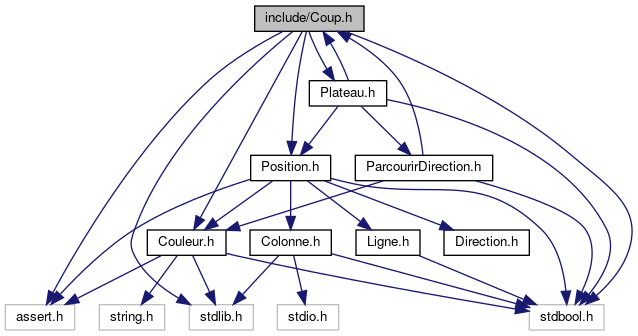
\includegraphics[width=350pt]{Coup_8h__incl}
\end{center}
\end{figure}
Ce graphe montre quels fichiers incluent directement ou indirectement ce fichier \+:
\nopagebreak
\begin{figure}[H]
\begin{center}
\leavevmode
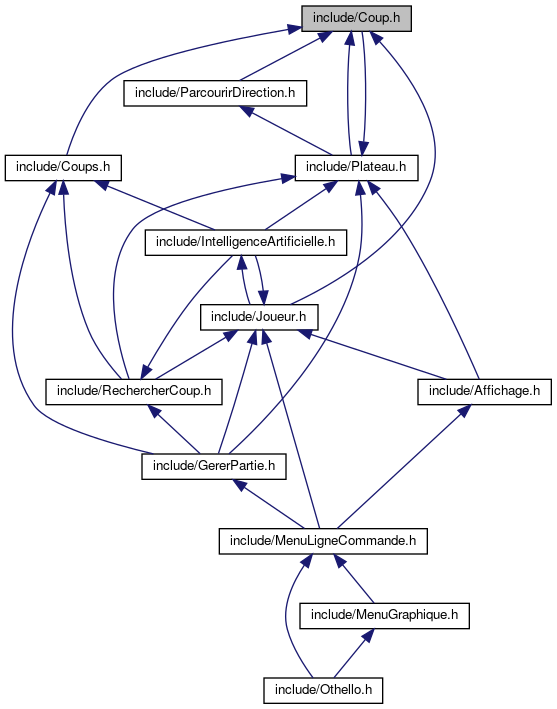
\includegraphics[width=350pt]{Coup_8h__dep__incl}
\end{center}
\end{figure}
\subsection*{Classes}
\begin{DoxyCompactItemize}
\item 
struct \hyperlink{structCoup}{Coup}
\begin{DoxyCompactList}\small\item\em Le type \hyperlink{structCoup}{Coup} permet de jouer une couleur à une position. \end{DoxyCompactList}\end{DoxyCompactItemize}
\subsection*{Fonctions}
\begin{DoxyCompactItemize}
\item 
\hyperlink{structCoup}{Coup} \hyperlink{Coup_8h_af23d663394bd9fede8f84b8c8159f129}{C\+O\+U\+P\+\_\+\+Creer\+Coup} (\hyperlink{structPosition}{Position} position, \hyperlink{structCouleur}{Couleur} couleur)
\begin{DoxyCompactList}\small\item\em Crée un \hyperlink{structCoup}{Coup}. \end{DoxyCompactList}\item 
bool \hyperlink{Coup_8h_addb431030561c86583c8163d02f2ae19}{C\+O\+U\+P\+\_\+\+Sont\+Egaux\+Coups} (\hyperlink{structCoup}{Coup} coup1, \hyperlink{structCoup}{Coup} coup2)
\begin{DoxyCompactList}\small\item\em Détermine si deux \hyperlink{structCoup}{Coup} sont identiques. \end{DoxyCompactList}\item 
\hyperlink{structCouleur}{Couleur} \hyperlink{Coup_8h_af0c3e47fcc4c12e2ebc0eeb7f28c37d6}{C\+O\+U\+P\+\_\+\+Obtenir\+Couleur} (\hyperlink{structCoup}{Coup} coup)
\begin{DoxyCompactList}\small\item\em Permet d\textquotesingle{}accéder au champs couleur d\textquotesingle{}une instance de \hyperlink{structCoup}{Coup}. \end{DoxyCompactList}\item 
\hyperlink{structPosition}{Position} \hyperlink{Coup_8h_ac930852f7ad3c8052fb9fdbf5f1db109}{C\+O\+U\+P\+\_\+\+Obtenir\+Position} (\hyperlink{structCoup}{Coup} coup)
\begin{DoxyCompactList}\small\item\em Permet d\textquotesingle{}accéder au champs position d\textquotesingle{}une instance de \hyperlink{structCoup}{Coup}. \end{DoxyCompactList}\item 
bool \hyperlink{Coup_8h_a9edbed93843ade7938339a2729c54fc7}{C\+O\+U\+P\+\_\+\+Est\+Coup\+Valide} (\hyperlink{structCouleur}{Couleur} $\ast$plateau, \hyperlink{structCoup}{Coup} coup)
\begin{DoxyCompactList}\small\item\em Détermine si un \hyperlink{structCoup}{Coup} est valide. \end{DoxyCompactList}\end{DoxyCompactItemize}


\subsection{Description détaillée}
Fichier contenant la définition du type \hyperlink{structCoup}{Coup} et de ses fonctions associées. 



\subsection{Documentation des fonctions}
\mbox{\Hypertarget{Coup_8h_af23d663394bd9fede8f84b8c8159f129}\label{Coup_8h_af23d663394bd9fede8f84b8c8159f129}} 
\index{Coup.\+h@{Coup.\+h}!C\+O\+U\+P\+\_\+\+Creer\+Coup@{C\+O\+U\+P\+\_\+\+Creer\+Coup}}
\index{C\+O\+U\+P\+\_\+\+Creer\+Coup@{C\+O\+U\+P\+\_\+\+Creer\+Coup}!Coup.\+h@{Coup.\+h}}
\subsubsection{\texorpdfstring{C\+O\+U\+P\+\_\+\+Creer\+Coup()}{COUP\_CreerCoup()}}
{\footnotesize\ttfamily \hyperlink{structCoup}{Coup} C\+O\+U\+P\+\_\+\+Creer\+Coup (\begin{DoxyParamCaption}\item[{\hyperlink{structPosition}{Position}}]{position,  }\item[{\hyperlink{structCouleur}{Couleur}}]{couleur }\end{DoxyParamCaption})}



Crée un \hyperlink{structCoup}{Coup}. 


\begin{DoxyParams}{Paramètres}
{\em position} & \hyperlink{structPosition}{Position} où le \hyperlink{structCoup}{Coup} doit être joué. \\
\hline
{\em couleur} & \hyperlink{structCouleur}{Couleur} du joueur qui joue le \hyperlink{structCoup}{Coup}.\\
\hline
\end{DoxyParams}
\begin{DoxyReturn}{Renvoie}
Instance de \hyperlink{structCoup}{Coup}. 
\end{DoxyReturn}
\mbox{\Hypertarget{Coup_8h_a9edbed93843ade7938339a2729c54fc7}\label{Coup_8h_a9edbed93843ade7938339a2729c54fc7}} 
\index{Coup.\+h@{Coup.\+h}!C\+O\+U\+P\+\_\+\+Est\+Coup\+Valide@{C\+O\+U\+P\+\_\+\+Est\+Coup\+Valide}}
\index{C\+O\+U\+P\+\_\+\+Est\+Coup\+Valide@{C\+O\+U\+P\+\_\+\+Est\+Coup\+Valide}!Coup.\+h@{Coup.\+h}}
\subsubsection{\texorpdfstring{C\+O\+U\+P\+\_\+\+Est\+Coup\+Valide()}{COUP\_EstCoupValide()}}
{\footnotesize\ttfamily bool C\+O\+U\+P\+\_\+\+Est\+Coup\+Valide (\begin{DoxyParamCaption}\item[{\hyperlink{structCouleur}{Couleur} $\ast$}]{plateau,  }\item[{\hyperlink{structCoup}{Coup}}]{coup }\end{DoxyParamCaption})}



Détermine si un \hyperlink{structCoup}{Coup} est valide. 

Il est considéré valide quand la position est elle même valide par rapport au plateau, et si la couleur du \hyperlink{structCoup}{Coup} n\textquotesingle{}est pas neutre.


\begin{DoxyParams}{Paramètres}
{\em plateau} & Plateau de jeu. \\
\hline
{\em coup} & \hyperlink{structCoup}{Coup} dont on souhaite tester la validité.\\
\hline
\end{DoxyParams}
\begin{DoxyReturn}{Renvoie}
true si le \hyperlink{structCoup}{Coup} est valide, false sinon. 
\end{DoxyReturn}
\mbox{\Hypertarget{Coup_8h_af0c3e47fcc4c12e2ebc0eeb7f28c37d6}\label{Coup_8h_af0c3e47fcc4c12e2ebc0eeb7f28c37d6}} 
\index{Coup.\+h@{Coup.\+h}!C\+O\+U\+P\+\_\+\+Obtenir\+Couleur@{C\+O\+U\+P\+\_\+\+Obtenir\+Couleur}}
\index{C\+O\+U\+P\+\_\+\+Obtenir\+Couleur@{C\+O\+U\+P\+\_\+\+Obtenir\+Couleur}!Coup.\+h@{Coup.\+h}}
\subsubsection{\texorpdfstring{C\+O\+U\+P\+\_\+\+Obtenir\+Couleur()}{COUP\_ObtenirCouleur()}}
{\footnotesize\ttfamily \hyperlink{structCouleur}{Couleur} C\+O\+U\+P\+\_\+\+Obtenir\+Couleur (\begin{DoxyParamCaption}\item[{\hyperlink{structCoup}{Coup}}]{coup }\end{DoxyParamCaption})}



Permet d\textquotesingle{}accéder au champs couleur d\textquotesingle{}une instance de \hyperlink{structCoup}{Coup}. 


\begin{DoxyParams}{Paramètres}
{\em coup} & \hyperlink{structCoup}{Coup} dont on souhaite obtenir la \hyperlink{structCouleur}{Couleur}.\\
\hline
\end{DoxyParams}
\begin{DoxyReturn}{Renvoie}
\hyperlink{structCouleur}{Couleur} du \hyperlink{structCoup}{Coup}. 
\end{DoxyReturn}
\mbox{\Hypertarget{Coup_8h_ac930852f7ad3c8052fb9fdbf5f1db109}\label{Coup_8h_ac930852f7ad3c8052fb9fdbf5f1db109}} 
\index{Coup.\+h@{Coup.\+h}!C\+O\+U\+P\+\_\+\+Obtenir\+Position@{C\+O\+U\+P\+\_\+\+Obtenir\+Position}}
\index{C\+O\+U\+P\+\_\+\+Obtenir\+Position@{C\+O\+U\+P\+\_\+\+Obtenir\+Position}!Coup.\+h@{Coup.\+h}}
\subsubsection{\texorpdfstring{C\+O\+U\+P\+\_\+\+Obtenir\+Position()}{COUP\_ObtenirPosition()}}
{\footnotesize\ttfamily \hyperlink{structPosition}{Position} C\+O\+U\+P\+\_\+\+Obtenir\+Position (\begin{DoxyParamCaption}\item[{\hyperlink{structCoup}{Coup}}]{coup }\end{DoxyParamCaption})}



Permet d\textquotesingle{}accéder au champs position d\textquotesingle{}une instance de \hyperlink{structCoup}{Coup}. 


\begin{DoxyParams}{Paramètres}
{\em coup} & \hyperlink{structCoup}{Coup} dont on souhaite obtenir la \hyperlink{structPosition}{Position}.\\
\hline
\end{DoxyParams}
\begin{DoxyReturn}{Renvoie}
\hyperlink{structPosition}{Position} du \hyperlink{structCoup}{Coup}. 
\end{DoxyReturn}
\mbox{\Hypertarget{Coup_8h_addb431030561c86583c8163d02f2ae19}\label{Coup_8h_addb431030561c86583c8163d02f2ae19}} 
\index{Coup.\+h@{Coup.\+h}!C\+O\+U\+P\+\_\+\+Sont\+Egaux\+Coups@{C\+O\+U\+P\+\_\+\+Sont\+Egaux\+Coups}}
\index{C\+O\+U\+P\+\_\+\+Sont\+Egaux\+Coups@{C\+O\+U\+P\+\_\+\+Sont\+Egaux\+Coups}!Coup.\+h@{Coup.\+h}}
\subsubsection{\texorpdfstring{C\+O\+U\+P\+\_\+\+Sont\+Egaux\+Coups()}{COUP\_SontEgauxCoups()}}
{\footnotesize\ttfamily bool C\+O\+U\+P\+\_\+\+Sont\+Egaux\+Coups (\begin{DoxyParamCaption}\item[{\hyperlink{structCoup}{Coup}}]{coup1,  }\item[{\hyperlink{structCoup}{Coup}}]{coup2 }\end{DoxyParamCaption})}



Détermine si deux \hyperlink{structCoup}{Coup} sont identiques. 


\begin{DoxyParams}{Paramètres}
{\em coup1} & Premier \hyperlink{structCoup}{Coup} à comparer. \\
\hline
{\em coup2} & Deuxième \hyperlink{structCoup}{Coup} à comparer.\\
\hline
\end{DoxyParams}
\begin{DoxyReturn}{Renvoie}
true si les \hyperlink{structCoup}{Coup} sont égaux, false sinon. 
\end{DoxyReturn}

\hypertarget{Coups_8h}{}\section{Référence du fichier include/\+Coups.h}
\label{Coups_8h}\index{include/\+Coups.\+h@{include/\+Coups.\+h}}


Fichier contenant la définition du type \hyperlink{structCoups}{Coups} et de ses fonctions associées.  


{\ttfamily \#include $<$stdbool.\+h$>$}\newline
{\ttfamily \#include $<$stdio.\+h$>$}\newline
{\ttfamily \#include \char`\"{}Coup.\+h\char`\"{}}\newline
Graphe des dépendances par inclusion de Coups.\+h\+:
\nopagebreak
\begin{figure}[H]
\begin{center}
\leavevmode
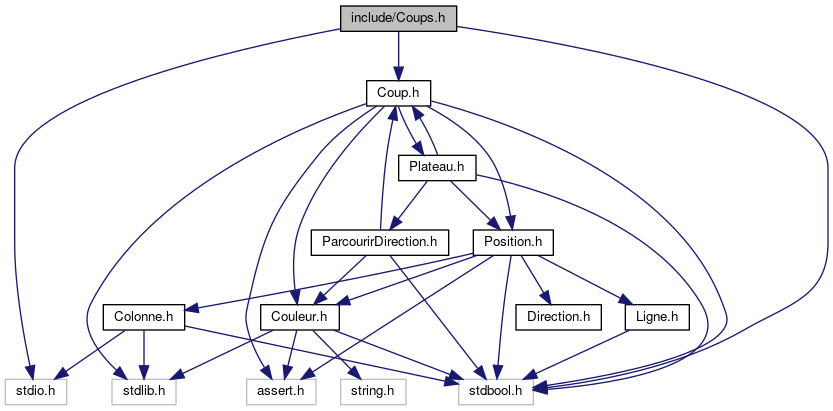
\includegraphics[width=350pt]{Coups_8h__incl}
\end{center}
\end{figure}
Ce graphe montre quels fichiers incluent directement ou indirectement ce fichier \+:
\nopagebreak
\begin{figure}[H]
\begin{center}
\leavevmode
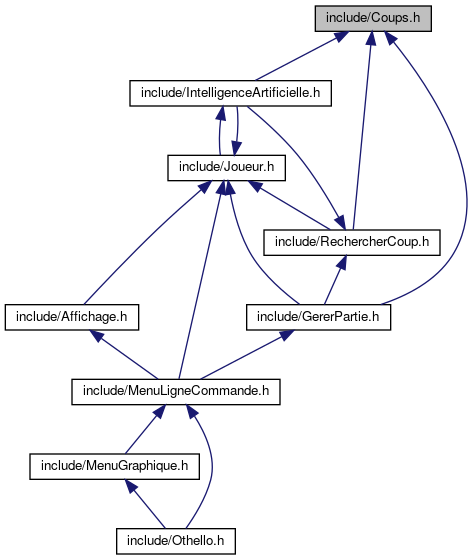
\includegraphics[width=350pt]{Coups_8h__dep__incl}
\end{center}
\end{figure}
\subsection*{Classes}
\begin{DoxyCompactItemize}
\item 
struct \hyperlink{structCoups}{Coups}
\begin{DoxyCompactList}\small\item\em Le type \hyperlink{structCoups}{Coups} permet de stocker plusieurs \hyperlink{structCoup}{Coup}. \end{DoxyCompactList}\end{DoxyCompactItemize}
\subsection*{Définitions de type}
\begin{DoxyCompactItemize}
\item 
typedef struct \hyperlink{structCoups}{Coups} \hyperlink{Coups_8h_a9234aaaeab8977b7d0405bf9fa7e0de0}{Coups}
\begin{DoxyCompactList}\small\item\em Le type \hyperlink{structCoups}{Coups} permet de stocker plusieurs \hyperlink{structCoup}{Coup}. \end{DoxyCompactList}\end{DoxyCompactItemize}
\subsection*{Fonctions}
\begin{DoxyCompactItemize}
\item 
\hyperlink{structCoups}{Coups} \hyperlink{Coups_8h_a182f348b22fe6709722563d3486803c5}{C\+O\+U\+P\+S\+\_\+\+Creer\+Coups} ()
\begin{DoxyCompactList}\small\item\em Crée une pile de \hyperlink{structCoup}{Coup}. \end{DoxyCompactList}\item 
bool \hyperlink{Coups_8h_af7bab4a0187f58e39953521d9d3a3046}{C\+O\+U\+P\+S\+\_\+\+Est\+Vide} (\hyperlink{structCoups}{Coups} coups)
\begin{DoxyCompactList}\small\item\em Détermine si \hyperlink{structCoups}{Coups} est vide, c\textquotesingle{}est à dire qu\textquotesingle{}il ne possède aucun \hyperlink{structCoup}{Coup}. \end{DoxyCompactList}\item 
void \hyperlink{Coups_8h_acbf64e939c28d8934dc22750cecfff34}{C\+O\+U\+P\+S\+\_\+\+Ajouter\+Coup} (\hyperlink{structCoups}{Coups} $\ast$p\+Coups, \hyperlink{structCoup}{Coup} coup)
\begin{DoxyCompactList}\small\item\em Ajoute un \hyperlink{structCoup}{Coup} à une instance de \hyperlink{structCoups}{Coups}. \end{DoxyCompactList}\item 
void \hyperlink{Coups_8h_a07e41b6f2bb5741ce3c84bda1111d254}{C\+O\+U\+P\+S\+\_\+\+Retirer\+Coup} (\hyperlink{structCoups}{Coups} $\ast$p\+Coups)
\begin{DoxyCompactList}\small\item\em Supprime un \hyperlink{structCoup}{Coup} d\textquotesingle{}une instance de \hyperlink{structCoups}{Coups}. \end{DoxyCompactList}\item 
\hyperlink{structCoup}{Coup} \hyperlink{Coups_8h_acaf697a0e6a06720fd5e1d4236d53af7}{C\+O\+U\+P\+S\+\_\+\+Obtenir\+Coup} (\hyperlink{structCoups}{Coups} coups)
\begin{DoxyCompactList}\small\item\em Permet d\textquotesingle{}obtenir un \hyperlink{structCoup}{Coup}. \end{DoxyCompactList}\item 
unsigned int \hyperlink{Coups_8h_af0876433a345cff704d9d1b400fd9e3d}{C\+O\+U\+P\+S\+\_\+\+Obtenir\+Nombre\+De\+Coups} (\hyperlink{structCoups}{Coups} coups)
\begin{DoxyCompactList}\small\item\em Permet de connaitre le nombre de \hyperlink{structCoup}{Coup} présents dans une pile \hyperlink{structCoups}{Coups}. \end{DoxyCompactList}\item 
bool \hyperlink{Coups_8h_a8153be7ff134057f2935173465a58da4}{C\+O\+U\+P\+S\+\_\+\+Est\+Present} (\hyperlink{structCoups}{Coups} coups, \hyperlink{structCoup}{Coup} coup)
\begin{DoxyCompactList}\small\item\em Détermine si un \hyperlink{structCoup}{Coup} est présent dans une Pile \hyperlink{structCoups}{Coups}. \end{DoxyCompactList}\end{DoxyCompactItemize}


\subsection{Description détaillée}
Fichier contenant la définition du type \hyperlink{structCoups}{Coups} et de ses fonctions associées. 

\begin{DoxyAuthor}{Auteur}
Léo Pacary 

Alexis Melo Da Silva 
\end{DoxyAuthor}


\subsection{Documentation des définitions de type}
\mbox{\Hypertarget{Coups_8h_a9234aaaeab8977b7d0405bf9fa7e0de0}\label{Coups_8h_a9234aaaeab8977b7d0405bf9fa7e0de0}} 
\index{Coups.\+h@{Coups.\+h}!Coups@{Coups}}
\index{Coups@{Coups}!Coups.\+h@{Coups.\+h}}
\subsubsection{\texorpdfstring{Coups}{Coups}}
{\footnotesize\ttfamily typedef struct \hyperlink{structCoups}{Coups} \hyperlink{structCoups}{Coups}}



Le type \hyperlink{structCoups}{Coups} permet de stocker plusieurs \hyperlink{structCoup}{Coup}. 

Sa manipulation s\textquotesingle{}apparente à celle d\textquotesingle{}une pile L\+I\+FO. 

\subsection{Documentation des fonctions}
\mbox{\Hypertarget{Coups_8h_acbf64e939c28d8934dc22750cecfff34}\label{Coups_8h_acbf64e939c28d8934dc22750cecfff34}} 
\index{Coups.\+h@{Coups.\+h}!C\+O\+U\+P\+S\+\_\+\+Ajouter\+Coup@{C\+O\+U\+P\+S\+\_\+\+Ajouter\+Coup}}
\index{C\+O\+U\+P\+S\+\_\+\+Ajouter\+Coup@{C\+O\+U\+P\+S\+\_\+\+Ajouter\+Coup}!Coups.\+h@{Coups.\+h}}
\subsubsection{\texorpdfstring{C\+O\+U\+P\+S\+\_\+\+Ajouter\+Coup()}{COUPS\_AjouterCoup()}}
{\footnotesize\ttfamily void C\+O\+U\+P\+S\+\_\+\+Ajouter\+Coup (\begin{DoxyParamCaption}\item[{\hyperlink{structCoups}{Coups} $\ast$}]{p\+Coups,  }\item[{\hyperlink{structCoup}{Coup}}]{coup }\end{DoxyParamCaption})}



Ajoute un \hyperlink{structCoup}{Coup} à une instance de \hyperlink{structCoups}{Coups}. 

Le \hyperlink{structCoup}{Coup} est ajouté en tête de pile.


\begin{DoxyParams}{Paramètres}
{\em p\+Coups} & Pointeur vers l\textquotesingle{}instance de \hyperlink{structCoups}{Coups} à laquelle on souhaite ajouter un \hyperlink{structCoup}{Coup}. \\
\hline
{\em coup} & \hyperlink{structCoup}{Coup} que l\textquotesingle{}on souhaite ajouter. \\
\hline
\end{DoxyParams}
\mbox{\Hypertarget{Coups_8h_a182f348b22fe6709722563d3486803c5}\label{Coups_8h_a182f348b22fe6709722563d3486803c5}} 
\index{Coups.\+h@{Coups.\+h}!C\+O\+U\+P\+S\+\_\+\+Creer\+Coups@{C\+O\+U\+P\+S\+\_\+\+Creer\+Coups}}
\index{C\+O\+U\+P\+S\+\_\+\+Creer\+Coups@{C\+O\+U\+P\+S\+\_\+\+Creer\+Coups}!Coups.\+h@{Coups.\+h}}
\subsubsection{\texorpdfstring{C\+O\+U\+P\+S\+\_\+\+Creer\+Coups()}{COUPS\_CreerCoups()}}
{\footnotesize\ttfamily \hyperlink{structCoups}{Coups} C\+O\+U\+P\+S\+\_\+\+Creer\+Coups (\begin{DoxyParamCaption}{ }\end{DoxyParamCaption})}



Crée une pile de \hyperlink{structCoup}{Coup}. 

\begin{DoxyReturn}{Renvoie}
Instance de \hyperlink{structCoups}{Coups}. 
\end{DoxyReturn}
\mbox{\Hypertarget{Coups_8h_a8153be7ff134057f2935173465a58da4}\label{Coups_8h_a8153be7ff134057f2935173465a58da4}} 
\index{Coups.\+h@{Coups.\+h}!C\+O\+U\+P\+S\+\_\+\+Est\+Present@{C\+O\+U\+P\+S\+\_\+\+Est\+Present}}
\index{C\+O\+U\+P\+S\+\_\+\+Est\+Present@{C\+O\+U\+P\+S\+\_\+\+Est\+Present}!Coups.\+h@{Coups.\+h}}
\subsubsection{\texorpdfstring{C\+O\+U\+P\+S\+\_\+\+Est\+Present()}{COUPS\_EstPresent()}}
{\footnotesize\ttfamily bool C\+O\+U\+P\+S\+\_\+\+Est\+Present (\begin{DoxyParamCaption}\item[{\hyperlink{structCoups}{Coups}}]{coups,  }\item[{\hyperlink{structCoup}{Coup}}]{coup }\end{DoxyParamCaption})}



Détermine si un \hyperlink{structCoup}{Coup} est présent dans une Pile \hyperlink{structCoups}{Coups}. 


\begin{DoxyParams}{Paramètres}
{\em coups} & Pile \hyperlink{structCoups}{Coups} dont on souhaite vérifier le contenu. \\
\hline
{\em coup} & \hyperlink{structCoup}{Coup} que l\textquotesingle{}on recherche.\\
\hline
\end{DoxyParams}
\begin{DoxyReturn}{Renvoie}
true si le coup est présent, false sinon. 
\end{DoxyReturn}
\mbox{\Hypertarget{Coups_8h_af7bab4a0187f58e39953521d9d3a3046}\label{Coups_8h_af7bab4a0187f58e39953521d9d3a3046}} 
\index{Coups.\+h@{Coups.\+h}!C\+O\+U\+P\+S\+\_\+\+Est\+Vide@{C\+O\+U\+P\+S\+\_\+\+Est\+Vide}}
\index{C\+O\+U\+P\+S\+\_\+\+Est\+Vide@{C\+O\+U\+P\+S\+\_\+\+Est\+Vide}!Coups.\+h@{Coups.\+h}}
\subsubsection{\texorpdfstring{C\+O\+U\+P\+S\+\_\+\+Est\+Vide()}{COUPS\_EstVide()}}
{\footnotesize\ttfamily bool C\+O\+U\+P\+S\+\_\+\+Est\+Vide (\begin{DoxyParamCaption}\item[{\hyperlink{structCoups}{Coups}}]{coups }\end{DoxyParamCaption})}



Détermine si \hyperlink{structCoups}{Coups} est vide, c\textquotesingle{}est à dire qu\textquotesingle{}il ne possède aucun \hyperlink{structCoup}{Coup}. 


\begin{DoxyParams}{Paramètres}
{\em coups} & Pile \hyperlink{structCoups}{Coups} dont on souhaite tester le contenu.\\
\hline
\end{DoxyParams}
\begin{DoxyReturn}{Renvoie}
true si \hyperlink{structCoups}{Coups} est vide, false sinon. 
\end{DoxyReturn}
\mbox{\Hypertarget{Coups_8h_acaf697a0e6a06720fd5e1d4236d53af7}\label{Coups_8h_acaf697a0e6a06720fd5e1d4236d53af7}} 
\index{Coups.\+h@{Coups.\+h}!C\+O\+U\+P\+S\+\_\+\+Obtenir\+Coup@{C\+O\+U\+P\+S\+\_\+\+Obtenir\+Coup}}
\index{C\+O\+U\+P\+S\+\_\+\+Obtenir\+Coup@{C\+O\+U\+P\+S\+\_\+\+Obtenir\+Coup}!Coups.\+h@{Coups.\+h}}
\subsubsection{\texorpdfstring{C\+O\+U\+P\+S\+\_\+\+Obtenir\+Coup()}{COUPS\_ObtenirCoup()}}
{\footnotesize\ttfamily \hyperlink{structCoup}{Coup} C\+O\+U\+P\+S\+\_\+\+Obtenir\+Coup (\begin{DoxyParamCaption}\item[{\hyperlink{structCoups}{Coups}}]{coups }\end{DoxyParamCaption})}



Permet d\textquotesingle{}obtenir un \hyperlink{structCoup}{Coup}. 

Obtient le coup en tête de pile.


\begin{DoxyParams}{Paramètres}
{\em coups} & Pile \hyperlink{structCoups}{Coups} dans laquelle on souhaite obtenir un \hyperlink{structCoup}{Coup}.\\
\hline
\end{DoxyParams}
\begin{DoxyReturn}{Renvoie}
Instance de \hyperlink{structCoup}{Coup} obtenue. 
\end{DoxyReturn}
\mbox{\Hypertarget{Coups_8h_af0876433a345cff704d9d1b400fd9e3d}\label{Coups_8h_af0876433a345cff704d9d1b400fd9e3d}} 
\index{Coups.\+h@{Coups.\+h}!C\+O\+U\+P\+S\+\_\+\+Obtenir\+Nombre\+De\+Coups@{C\+O\+U\+P\+S\+\_\+\+Obtenir\+Nombre\+De\+Coups}}
\index{C\+O\+U\+P\+S\+\_\+\+Obtenir\+Nombre\+De\+Coups@{C\+O\+U\+P\+S\+\_\+\+Obtenir\+Nombre\+De\+Coups}!Coups.\+h@{Coups.\+h}}
\subsubsection{\texorpdfstring{C\+O\+U\+P\+S\+\_\+\+Obtenir\+Nombre\+De\+Coups()}{COUPS\_ObtenirNombreDeCoups()}}
{\footnotesize\ttfamily unsigned int C\+O\+U\+P\+S\+\_\+\+Obtenir\+Nombre\+De\+Coups (\begin{DoxyParamCaption}\item[{\hyperlink{structCoups}{Coups}}]{coups }\end{DoxyParamCaption})}



Permet de connaitre le nombre de \hyperlink{structCoup}{Coup} présents dans une pile \hyperlink{structCoups}{Coups}. 


\begin{DoxyParams}{Paramètres}
{\em coups} & Pile \hyperlink{structCoups}{Coups} dont on souhaite connaitre le nombre de \hyperlink{structCoup}{Coup}.\\
\hline
\end{DoxyParams}
\begin{DoxyReturn}{Renvoie}
Nombre de \hyperlink{structCoup}{Coup}. 
\end{DoxyReturn}
\mbox{\Hypertarget{Coups_8h_a07e41b6f2bb5741ce3c84bda1111d254}\label{Coups_8h_a07e41b6f2bb5741ce3c84bda1111d254}} 
\index{Coups.\+h@{Coups.\+h}!C\+O\+U\+P\+S\+\_\+\+Retirer\+Coup@{C\+O\+U\+P\+S\+\_\+\+Retirer\+Coup}}
\index{C\+O\+U\+P\+S\+\_\+\+Retirer\+Coup@{C\+O\+U\+P\+S\+\_\+\+Retirer\+Coup}!Coups.\+h@{Coups.\+h}}
\subsubsection{\texorpdfstring{C\+O\+U\+P\+S\+\_\+\+Retirer\+Coup()}{COUPS\_RetirerCoup()}}
{\footnotesize\ttfamily void C\+O\+U\+P\+S\+\_\+\+Retirer\+Coup (\begin{DoxyParamCaption}\item[{\hyperlink{structCoups}{Coups} $\ast$}]{p\+Coups }\end{DoxyParamCaption})}



Supprime un \hyperlink{structCoup}{Coup} d\textquotesingle{}une instance de \hyperlink{structCoups}{Coups}. 

Le coup supprimé est celui en tête de pile.


\begin{DoxyParams}{Paramètres}
{\em p\+Coups} & Pointeur vers l\textquotesingle{}instance de \hyperlink{structCoups}{Coups} à laquelle on souhaite retirer un coup. \\
\hline
\end{DoxyParams}

\hypertarget{Direction_8h}{}\section{Référence du fichier include/\+Direction.h}
\label{Direction_8h}\index{include/\+Direction.\+h@{include/\+Direction.\+h}}


Fichier contenant la définition de l\textquotesingle{}enum Direction et de ses fonctions associées.  


Ce graphe montre quels fichiers incluent directement ou indirectement ce fichier \+:
\nopagebreak
\begin{figure}[H]
\begin{center}
\leavevmode
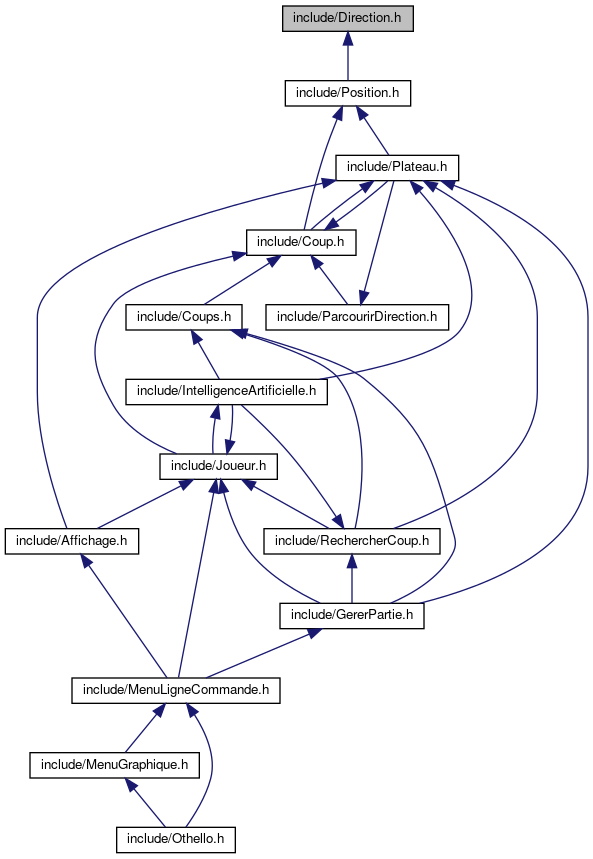
\includegraphics[width=350pt]{Direction_8h__dep__incl}
\end{center}
\end{figure}
\subsection*{Macros}
\begin{DoxyCompactItemize}
\item 
\mbox{\Hypertarget{Direction_8h_a3d952ccde2f2c145d3d0dfa423add90d}\label{Direction_8h_a3d952ccde2f2c145d3d0dfa423add90d}} 
\#define {\bfseries D\+I\+R\+E\+C\+T\+I\+O\+N\+\_\+\+E\+R\+R\+OR}~-\/1;
\end{DoxyCompactItemize}
\subsection*{Énumérations}
\begin{DoxyCompactItemize}
\item 
\mbox{\Hypertarget{Direction_8h_a224b9163917ac32fc95a60d8c1eec3aa}\label{Direction_8h_a224b9163917ac32fc95a60d8c1eec3aa}} 
enum \hyperlink{Direction_8h_a224b9163917ac32fc95a60d8c1eec3aa}{Direction} \{ \newline
{\bfseries H}, 
{\bfseries HD}, 
{\bfseries D}, 
{\bfseries BD}, 
\newline
{\bfseries B}, 
{\bfseries BG}, 
{\bfseries G}, 
{\bfseries HG}
 \}\begin{DoxyCompactList}\small\item\em L\textquotesingle{}énumeration Direction permet de manipuler des coordonnées relatives à un point central pour obtenir un décalage de Ligne ou de Colonne compris entre -\/1 et 1. \end{DoxyCompactList}
\end{DoxyCompactItemize}
\subsection*{Fonctions}
\begin{DoxyCompactItemize}
\item 
int \hyperlink{Direction_8h_af839bfa485b9a0ace035eebb3b3ff904}{Obtenir\+Decalage\+Ligne} (\hyperlink{Direction_8h_a224b9163917ac32fc95a60d8c1eec3aa}{Direction} direction)
\begin{DoxyCompactList}\small\item\em Permet d\textquotesingle{}obtenir le décalage au niveau d\textquotesingle{}une Ligne qu\textquotesingle{}implique une direction donnée. \end{DoxyCompactList}\item 
int \hyperlink{Direction_8h_aae124d99bb1878e43a057b644dfd4679}{Obtenir\+Decalage\+Colonne} (\hyperlink{Direction_8h_a224b9163917ac32fc95a60d8c1eec3aa}{Direction} direction)
\begin{DoxyCompactList}\small\item\em Permet d\textquotesingle{}obtenir le décalage au niveau d\textquotesingle{}une Colonne qu\textquotesingle{}implique une direction donnée. \end{DoxyCompactList}\end{DoxyCompactItemize}


\subsection{Description détaillée}
Fichier contenant la définition de l\textquotesingle{}enum Direction et de ses fonctions associées. 



\subsection{Documentation des fonctions}
\mbox{\Hypertarget{Direction_8h_aae124d99bb1878e43a057b644dfd4679}\label{Direction_8h_aae124d99bb1878e43a057b644dfd4679}} 
\index{Direction.\+h@{Direction.\+h}!Obtenir\+Decalage\+Colonne@{Obtenir\+Decalage\+Colonne}}
\index{Obtenir\+Decalage\+Colonne@{Obtenir\+Decalage\+Colonne}!Direction.\+h@{Direction.\+h}}
\subsubsection{\texorpdfstring{Obtenir\+Decalage\+Colonne()}{ObtenirDecalageColonne()}}
{\footnotesize\ttfamily int Obtenir\+Decalage\+Colonne (\begin{DoxyParamCaption}\item[{\hyperlink{Direction_8h_a224b9163917ac32fc95a60d8c1eec3aa}{Direction}}]{direction }\end{DoxyParamCaption})}



Permet d\textquotesingle{}obtenir le décalage au niveau d\textquotesingle{}une Colonne qu\textquotesingle{}implique une direction donnée. 


\begin{DoxyParams}{Paramètres}
{\em direction} & Direction dont on souhaite obtenir le décalage.\\
\hline
\end{DoxyParams}
\begin{DoxyReturn}{Renvoie}
Integer correspondant au décalage 
\end{DoxyReturn}
\mbox{\Hypertarget{Direction_8h_af839bfa485b9a0ace035eebb3b3ff904}\label{Direction_8h_af839bfa485b9a0ace035eebb3b3ff904}} 
\index{Direction.\+h@{Direction.\+h}!Obtenir\+Decalage\+Ligne@{Obtenir\+Decalage\+Ligne}}
\index{Obtenir\+Decalage\+Ligne@{Obtenir\+Decalage\+Ligne}!Direction.\+h@{Direction.\+h}}
\subsubsection{\texorpdfstring{Obtenir\+Decalage\+Ligne()}{ObtenirDecalageLigne()}}
{\footnotesize\ttfamily int Obtenir\+Decalage\+Ligne (\begin{DoxyParamCaption}\item[{\hyperlink{Direction_8h_a224b9163917ac32fc95a60d8c1eec3aa}{Direction}}]{direction }\end{DoxyParamCaption})}



Permet d\textquotesingle{}obtenir le décalage au niveau d\textquotesingle{}une Ligne qu\textquotesingle{}implique une direction donnée. 


\begin{DoxyParams}{Paramètres}
{\em direction} & Direction dont on souhaite obtenir le décalage.\\
\hline
\end{DoxyParams}
\begin{DoxyReturn}{Renvoie}
Integer correspondant au décalage 
\end{DoxyReturn}

\hypertarget{GererPartie_8h}{}\section{Référence du fichier include/\+Gerer\+Partie.h}
\label{GererPartie_8h}\index{include/\+Gerer\+Partie.\+h@{include/\+Gerer\+Partie.\+h}}


Fichier contenant la définition des fonctions permettant de gérer le déroulement d\textquotesingle{}une partie d\textquotesingle{}Othello.  


{\ttfamily \#include \char`\"{}Couleur.\+h\char`\"{}}\newline
{\ttfamily \#include \char`\"{}Plateau.\+h\char`\"{}}\newline
{\ttfamily \#include \char`\"{}Joueur.\+h\char`\"{}}\newline
{\ttfamily \#include \char`\"{}Coups.\+h\char`\"{}}\newline
{\ttfamily \#include \char`\"{}Rechercher\+Coup.\+h\char`\"{}}\newline
Graphe des dépendances par inclusion de Gerer\+Partie.\+h\+:
\nopagebreak
\begin{figure}[H]
\begin{center}
\leavevmode
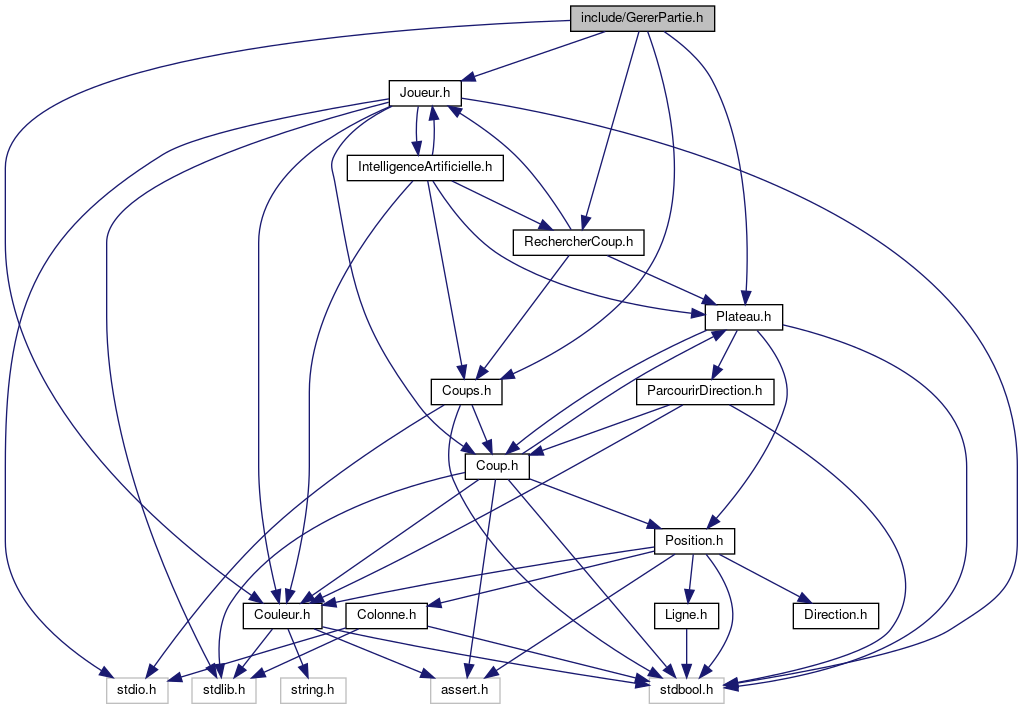
\includegraphics[width=350pt]{GererPartie_8h__incl}
\end{center}
\end{figure}
Ce graphe montre quels fichiers incluent directement ou indirectement ce fichier \+:
\nopagebreak
\begin{figure}[H]
\begin{center}
\leavevmode
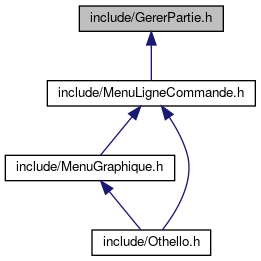
\includegraphics[width=268pt]{GererPartie_8h__dep__incl}
\end{center}
\end{figure}
\subsection*{Fonctions}
\begin{DoxyCompactItemize}
\item 
\mbox{\Hypertarget{GererPartie_8h_ac2214e7b28f2ebb39ca008254dc30fa9}\label{GererPartie_8h_ac2214e7b28f2ebb39ca008254dc30fa9}} 
void {\bfseries P\+A\+R\+T\+I\+E\+\_\+\+Faire\+Une\+Partie} (void($\ast$Afficher\+Resultat)(\hyperlink{structCouleur}{Couleur} $\ast$, \hyperlink{structJoueur}{Joueur}, \hyperlink{structJoueur}{Joueur}), void($\ast$Afficher\+Plateau)(\hyperlink{structCouleur}{Couleur} $\ast$), void($\ast$Afficher\+Coup)(\hyperlink{structCoup}{Coup}), void($\ast$Afficher\+Saisie\+Coup)(\hyperlink{structJoueur}{Joueur}), \hyperlink{structJoueur}{Joueur} j1, \hyperlink{structJoueur}{Joueur} j2)
\item 
void \hyperlink{GererPartie_8h_a3673aa9f7dd0787766a2dbee1415671d}{P\+A\+R\+T\+I\+E\+\_\+\+Gerer\+Partie} (void($\ast$Afficher\+Resultat)(\hyperlink{structCouleur}{Couleur} $\ast$, \hyperlink{structJoueur}{Joueur}, \hyperlink{structJoueur}{Joueur}), void($\ast$Afficher\+Plateau)(\hyperlink{structCouleur}{Couleur} $\ast$), void($\ast$Afficher\+Coup)(\hyperlink{structCoup}{Coup}), void($\ast$Afficher\+Saisie\+Coup)(\hyperlink{structJoueur}{Joueur}), \hyperlink{structJoueur}{Joueur} j1, \hyperlink{structJoueur}{Joueur} j2, \hyperlink{structCouleur}{Couleur} $\ast$plateau)
\begin{DoxyCompactList}\small\item\em Permet de gérer une partie cad alterner les tours, savoir si elle est finie, etc... \end{DoxyCompactList}\item 
void \hyperlink{GererPartie_8h_a913c62c910308febc783c36a558d4e82}{P\+A\+R\+T\+I\+E\+\_\+\+Set\+Ordre\+Joueurs} (\hyperlink{structJoueur}{Joueur} $\ast$premier\+Joueur, \hyperlink{structJoueur}{Joueur} $\ast$second\+Joueur, \hyperlink{structJoueur}{Joueur} j1, \hyperlink{structJoueur}{Joueur} j2)
\begin{DoxyCompactList}\small\item\em Initialise les valeurs des pointeurs premier\+Joueur et second\+Joueur avec les valeurs de j1 et de j2, sachant que c\textquotesingle{}est toujours le joueur de couleur noire qui doit commencer la partie. \end{DoxyCompactList}\item 
void \hyperlink{GererPartie_8h_ae58c6695548ea93298a5bfb1851c9bc7}{P\+A\+R\+T\+I\+E\+\_\+\+Jouer\+Un\+Tour} (\hyperlink{structCouleur}{Couleur} $\ast$plateau, \hyperlink{structJoueur}{Joueur} joueur, void($\ast$Afficher\+Coup)(\hyperlink{structCoup}{Coup}), void($\ast$Afficher\+Saisie\+Coup)(\hyperlink{structJoueur}{Joueur}))
\begin{DoxyCompactList}\small\item\em Permet d\textquotesingle{}obtenir un coup de la part d\textquotesingle{}un joueur et de le jouer sur plateau. \end{DoxyCompactList}\end{DoxyCompactItemize}


\subsection{Description détaillée}
Fichier contenant la définition des fonctions permettant de gérer le déroulement d\textquotesingle{}une partie d\textquotesingle{}Othello. 



\subsection{Documentation des fonctions}
\mbox{\Hypertarget{GererPartie_8h_a3673aa9f7dd0787766a2dbee1415671d}\label{GererPartie_8h_a3673aa9f7dd0787766a2dbee1415671d}} 
\index{Gerer\+Partie.\+h@{Gerer\+Partie.\+h}!P\+A\+R\+T\+I\+E\+\_\+\+Gerer\+Partie@{P\+A\+R\+T\+I\+E\+\_\+\+Gerer\+Partie}}
\index{P\+A\+R\+T\+I\+E\+\_\+\+Gerer\+Partie@{P\+A\+R\+T\+I\+E\+\_\+\+Gerer\+Partie}!Gerer\+Partie.\+h@{Gerer\+Partie.\+h}}
\subsubsection{\texorpdfstring{P\+A\+R\+T\+I\+E\+\_\+\+Gerer\+Partie()}{PARTIE\_GererPartie()}}
{\footnotesize\ttfamily void P\+A\+R\+T\+I\+E\+\_\+\+Gerer\+Partie (\begin{DoxyParamCaption}\item[{void($\ast$)(\hyperlink{structCouleur}{Couleur} $\ast$, \hyperlink{structJoueur}{Joueur}, \hyperlink{structJoueur}{Joueur})}]{Afficher\+Resultat,  }\item[{void($\ast$)(\hyperlink{structCouleur}{Couleur} $\ast$)}]{Afficher\+Plateau,  }\item[{void($\ast$)(\hyperlink{structCoup}{Coup})}]{Afficher\+Coup,  }\item[{void($\ast$)(\hyperlink{structJoueur}{Joueur})}]{Afficher\+Saisie\+Coup,  }\item[{\hyperlink{structJoueur}{Joueur}}]{j1,  }\item[{\hyperlink{structJoueur}{Joueur}}]{j2,  }\item[{\hyperlink{structCouleur}{Couleur} $\ast$}]{plateau }\end{DoxyParamCaption})}



Permet de gérer une partie cad alterner les tours, savoir si elle est finie, etc... 


\begin{DoxyParams}{Paramètres}
{\em Afficher\+Resultat} & Pointeur de fonction pour afficher les résultats de fin de partie. \\
\hline
{\em Afficher\+Plateau} & Pointeur de fonction pour afficher le plateau. \\
\hline
{\em Afficher\+Coup} & Pointeur de fonction pour afficher le coup qui viens d\textquotesingle{}être joué \\
\hline
{\em Afficher\+Saisie\+Coup} & Pointeur de fonction pour afficher la demande de saisie d\textquotesingle{}un coup \\
\hline
{\em j1} & Premier \hyperlink{structJoueur}{Joueur}. \\
\hline
{\em j2} & Second \hyperlink{structJoueur}{Joueur}. \\
\hline
{\em plateau} & Plateau de jeu initialisé. \\
\hline
\end{DoxyParams}
\mbox{\Hypertarget{GererPartie_8h_ae58c6695548ea93298a5bfb1851c9bc7}\label{GererPartie_8h_ae58c6695548ea93298a5bfb1851c9bc7}} 
\index{Gerer\+Partie.\+h@{Gerer\+Partie.\+h}!P\+A\+R\+T\+I\+E\+\_\+\+Jouer\+Un\+Tour@{P\+A\+R\+T\+I\+E\+\_\+\+Jouer\+Un\+Tour}}
\index{P\+A\+R\+T\+I\+E\+\_\+\+Jouer\+Un\+Tour@{P\+A\+R\+T\+I\+E\+\_\+\+Jouer\+Un\+Tour}!Gerer\+Partie.\+h@{Gerer\+Partie.\+h}}
\subsubsection{\texorpdfstring{P\+A\+R\+T\+I\+E\+\_\+\+Jouer\+Un\+Tour()}{PARTIE\_JouerUnTour()}}
{\footnotesize\ttfamily void P\+A\+R\+T\+I\+E\+\_\+\+Jouer\+Un\+Tour (\begin{DoxyParamCaption}\item[{\hyperlink{structCouleur}{Couleur} $\ast$}]{plateau,  }\item[{\hyperlink{structJoueur}{Joueur}}]{joueur,  }\item[{void($\ast$)(\hyperlink{structCoup}{Coup})}]{Afficher\+Coup,  }\item[{void($\ast$)(\hyperlink{structJoueur}{Joueur})}]{Afficher\+Saisie\+Coup }\end{DoxyParamCaption})}



Permet d\textquotesingle{}obtenir un coup de la part d\textquotesingle{}un joueur et de le jouer sur plateau. 


\begin{DoxyParams}{Paramètres}
{\em plateau} & Plateau de jeu. \\
\hline
{\em joueur} & \hyperlink{structJoueur}{Joueur} qui doit jouer pendant ce tour. \\
\hline
{\em Afficher\+Coup} & Pointeur de fonction pour afficher le déroulement d\textquotesingle{}un \hyperlink{structCoup}{Coup}. \\
\hline
{\em Afficher\+Saisie\+Coup} & Pointeur de fonction pour afficher la demande de saisie d\textquotesingle{}un coup \\
\hline
\end{DoxyParams}
\mbox{\Hypertarget{GererPartie_8h_a913c62c910308febc783c36a558d4e82}\label{GererPartie_8h_a913c62c910308febc783c36a558d4e82}} 
\index{Gerer\+Partie.\+h@{Gerer\+Partie.\+h}!P\+A\+R\+T\+I\+E\+\_\+\+Set\+Ordre\+Joueurs@{P\+A\+R\+T\+I\+E\+\_\+\+Set\+Ordre\+Joueurs}}
\index{P\+A\+R\+T\+I\+E\+\_\+\+Set\+Ordre\+Joueurs@{P\+A\+R\+T\+I\+E\+\_\+\+Set\+Ordre\+Joueurs}!Gerer\+Partie.\+h@{Gerer\+Partie.\+h}}
\subsubsection{\texorpdfstring{P\+A\+R\+T\+I\+E\+\_\+\+Set\+Ordre\+Joueurs()}{PARTIE\_SetOrdreJoueurs()}}
{\footnotesize\ttfamily void P\+A\+R\+T\+I\+E\+\_\+\+Set\+Ordre\+Joueurs (\begin{DoxyParamCaption}\item[{\hyperlink{structJoueur}{Joueur} $\ast$}]{premier\+Joueur,  }\item[{\hyperlink{structJoueur}{Joueur} $\ast$}]{second\+Joueur,  }\item[{\hyperlink{structJoueur}{Joueur}}]{j1,  }\item[{\hyperlink{structJoueur}{Joueur}}]{j2 }\end{DoxyParamCaption})}



Initialise les valeurs des pointeurs premier\+Joueur et second\+Joueur avec les valeurs de j1 et de j2, sachant que c\textquotesingle{}est toujours le joueur de couleur noire qui doit commencer la partie. 


\begin{DoxyParams}{Paramètres}
{\em premier\+Joueur} & \hyperlink{structJoueur}{Joueur} qui doit jouer en premier dans la partie. \\
\hline
{\em second\+Joueur} & \hyperlink{structJoueur}{Joueur} qui doit jouer en second dans la partie. \\
\hline
{\em j1} & \hyperlink{structJoueur}{Joueur} numéro 1, qui n\textquotesingle{}est pas forcément le premier à jouer. \\
\hline
{\em j2} & \hyperlink{structJoueur}{Joueur} numéro 2. \\
\hline
\end{DoxyParams}

\hypertarget{IntelligenceArtificielle_8h}{}\section{Référence du fichier include/\+Intelligence\+Artificielle.h}
\label{IntelligenceArtificielle_8h}\index{include/\+Intelligence\+Artificielle.\+h@{include/\+Intelligence\+Artificielle.\+h}}


Fichier contenant la définition des fonctions pour obtenir un \hyperlink{structCoup}{Coup} d\textquotesingle{}une IA.  


{\ttfamily \#include \char`\"{}Plateau.\+h\char`\"{}}\newline
{\ttfamily \#include \char`\"{}Joueur.\+h\char`\"{}}\newline
{\ttfamily \#include \char`\"{}Coups.\+h\char`\"{}}\newline
{\ttfamily \#include \char`\"{}Rechercher\+Coup.\+h\char`\"{}}\newline
{\ttfamily \#include \char`\"{}Couleur.\+h\char`\"{}}\newline
Graphe des dépendances par inclusion de Intelligence\+Artificielle.\+h\+:
\nopagebreak
\begin{figure}[H]
\begin{center}
\leavevmode
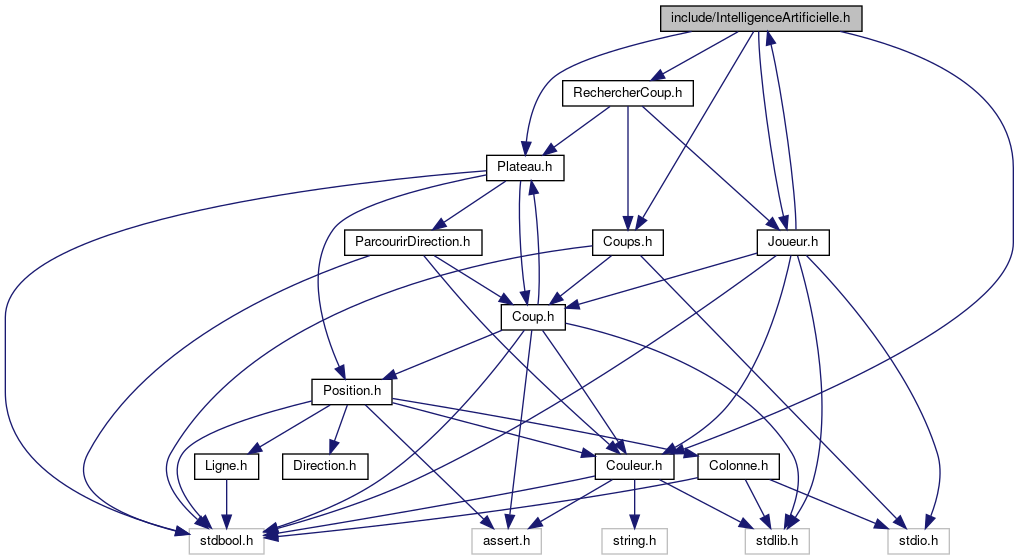
\includegraphics[width=350pt]{IntelligenceArtificielle_8h__incl}
\end{center}
\end{figure}
Ce graphe montre quels fichiers incluent directement ou indirectement ce fichier \+:
\nopagebreak
\begin{figure}[H]
\begin{center}
\leavevmode
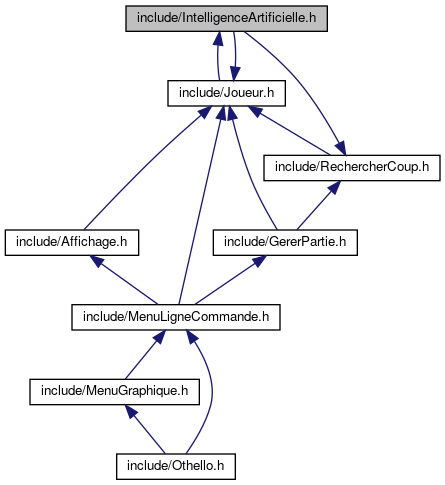
\includegraphics[width=350pt]{IntelligenceArtificielle_8h__dep__incl}
\end{center}
\end{figure}
\subsection*{Fonctions}
\begin{DoxyCompactItemize}
\item 
\hyperlink{structCoup}{Coup} \hyperlink{IntelligenceArtificielle_8h_a799512a1c957a2bb61227007284370ca}{I\+A\+\_\+\+Min\+Max} (\hyperlink{structCouleur}{Couleur} $\ast$plateau, \hyperlink{structJoueur}{Joueur} joueur\+A\+Maximiser, int profondeur)
\begin{DoxyCompactList}\small\item\em Permet d\textquotesingle{}obtenir un \hyperlink{structCoup}{Coup} par une IA. \end{DoxyCompactList}\item 
\mbox{\Hypertarget{IntelligenceArtificielle_8h_a8e4a56f42aef3c4a4931a7469308f5ed}\label{IntelligenceArtificielle_8h_a8e4a56f42aef3c4a4931a7469308f5ed}} 
\hyperlink{structCoup}{Coup} {\bfseries I\+A\+\_\+\+Alpha\+Beta} (\hyperlink{structCouleur}{Couleur} $\ast$plateau, \hyperlink{structJoueur}{Joueur} joueur\+A\+Maximiser, int Profondeur)
\end{DoxyCompactItemize}


\subsection{Description détaillée}
Fichier contenant la définition des fonctions pour obtenir un \hyperlink{structCoup}{Coup} d\textquotesingle{}une IA. 



\subsection{Documentation des fonctions}
\mbox{\Hypertarget{IntelligenceArtificielle_8h_a799512a1c957a2bb61227007284370ca}\label{IntelligenceArtificielle_8h_a799512a1c957a2bb61227007284370ca}} 
\index{Intelligence\+Artificielle.\+h@{Intelligence\+Artificielle.\+h}!I\+A\+\_\+\+Min\+Max@{I\+A\+\_\+\+Min\+Max}}
\index{I\+A\+\_\+\+Min\+Max@{I\+A\+\_\+\+Min\+Max}!Intelligence\+Artificielle.\+h@{Intelligence\+Artificielle.\+h}}
\subsubsection{\texorpdfstring{I\+A\+\_\+\+Min\+Max()}{IA\_MinMax()}}
{\footnotesize\ttfamily \hyperlink{structCoup}{Coup} I\+A\+\_\+\+Min\+Max (\begin{DoxyParamCaption}\item[{\hyperlink{structCouleur}{Couleur} $\ast$}]{plateau,  }\item[{\hyperlink{structJoueur}{Joueur}}]{joueur\+A\+Maximiser,  }\item[{int}]{profondeur }\end{DoxyParamCaption})}



Permet d\textquotesingle{}obtenir un \hyperlink{structCoup}{Coup} par une IA. 

Le \hyperlink{structCoup}{Coup} est calculé automatiquement, la profondeur permet de spécifier combien de \hyperlink{structCoup}{Coup} à l\textquotesingle{}avance l\textquotesingle{}IA peut calculer son coup, sachant que plus ce nombre est élevé plus l\textquotesingle{}IA sera lente à répondre.


\begin{DoxyParams}{Paramètres}
{\em plateau} & Plateau de jeu \\
\hline
{\em joueur\+A\+Maximiser} & \hyperlink{structJoueur}{Joueur} dont on souhaite obtenir le meilleur coup possible \\
\hline
{\em profondeur} & Profondeur de recherche de l\textquotesingle{}IA\\
\hline
\end{DoxyParams}
\begin{DoxyReturn}{Renvoie}
Meilleur \hyperlink{structCoup}{Coup} obtenu par l\textquotesingle{}IA 
\end{DoxyReturn}

\hypertarget{Joueur_8h}{}\section{Référence du fichier include/\+Joueur.h}
\label{Joueur_8h}\index{include/\+Joueur.\+h@{include/\+Joueur.\+h}}


Fichier contenant la définition du type \hyperlink{structJoueur}{Joueur} et de ses fonctions associées.  


{\ttfamily \#include $<$stdbool.\+h$>$}\newline
{\ttfamily \#include $<$stdlib.\+h$>$}\newline
{\ttfamily \#include $<$stdio.\+h$>$}\newline
{\ttfamily \#include \char`\"{}Couleur.\+h\char`\"{}}\newline
{\ttfamily \#include \char`\"{}Coup.\+h\char`\"{}}\newline
{\ttfamily \#include \char`\"{}Intelligence\+Artificielle.\+h\char`\"{}}\newline
Graphe des dépendances par inclusion de Joueur.\+h\+:
\nopagebreak
\begin{figure}[H]
\begin{center}
\leavevmode
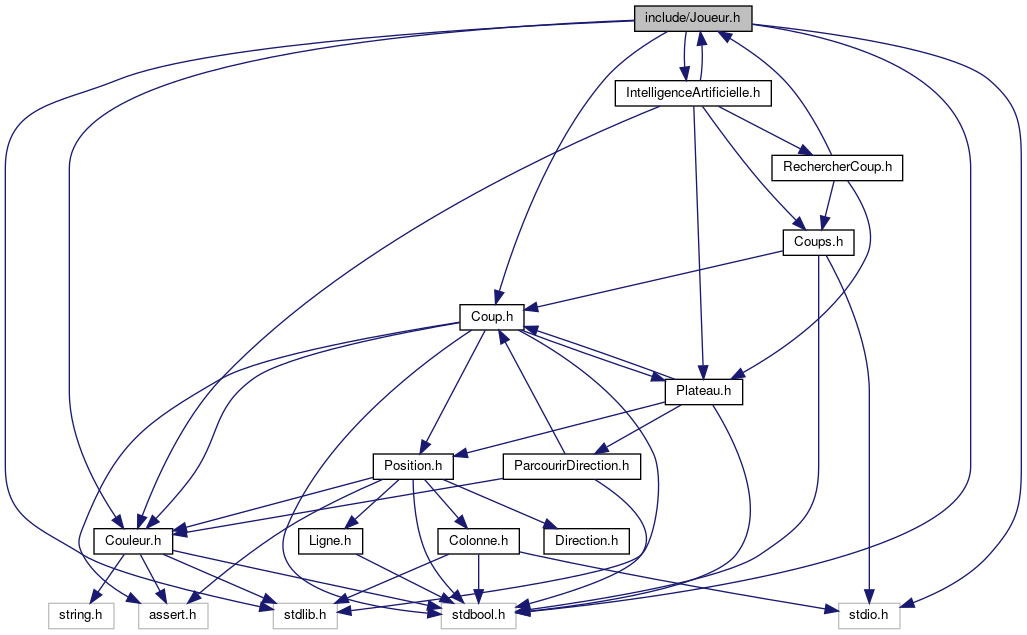
\includegraphics[width=350pt]{Joueur_8h__incl}
\end{center}
\end{figure}
Ce graphe montre quels fichiers incluent directement ou indirectement ce fichier \+:
\nopagebreak
\begin{figure}[H]
\begin{center}
\leavevmode
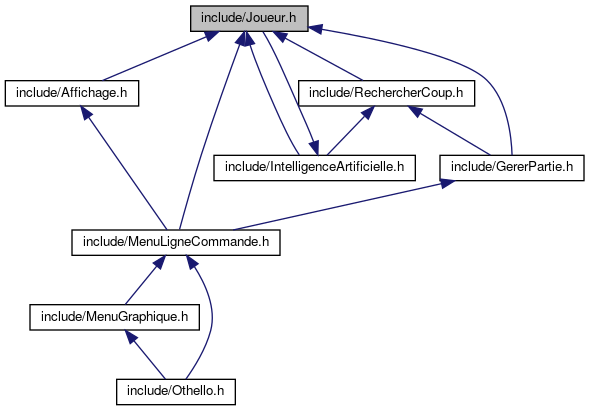
\includegraphics[width=350pt]{Joueur_8h__dep__incl}
\end{center}
\end{figure}
\subsection*{Classes}
\begin{DoxyCompactItemize}
\item 
struct \hyperlink{structJoueur}{Joueur}
\begin{DoxyCompactList}\small\item\em Le type \hyperlink{structJoueur}{Joueur} permet de manipuler une couleur en sachant si elle est jouée par une IA ou un \hyperlink{structJoueur}{Joueur} réel. \end{DoxyCompactList}\end{DoxyCompactItemize}
\subsection*{Fonctions}
\begin{DoxyCompactItemize}
\item 
\hyperlink{structJoueur}{Joueur} \hyperlink{Joueur_8h_a4df13be25c1cf218785dc9edd1134390}{J\+O\+U\+E\+U\+R\+\_\+\+Creer\+Joueur\+Humain} (\hyperlink{structCouleur}{Couleur} couleur)
\begin{DoxyCompactList}\small\item\em Crée un \hyperlink{structJoueur}{Joueur} joué par un humain. \end{DoxyCompactList}\item 
\hyperlink{structJoueur}{Joueur} \hyperlink{Joueur_8h_a418fd1c5d250f5a47420b60f3f771939}{J\+O\+U\+E\+U\+R\+\_\+\+Creer\+Joueur\+IA} (\hyperlink{structCouleur}{Couleur} couleur, int profondeur)
\begin{DoxyCompactList}\small\item\em Crée un \hyperlink{structJoueur}{Joueur} joué par une IA. \end{DoxyCompactList}\item 
\hyperlink{structCoup}{Coup} \hyperlink{Joueur_8h_a3af76f7b5fc6bec9be5c3ff8d4ab42fe}{J\+O\+U\+E\+U\+R\+\_\+\+Saisir\+Coup\+Humain} (\hyperlink{structJoueur}{Joueur} joueur)
\begin{DoxyCompactList}\small\item\em Permet d\textquotesingle{}obtenir un \hyperlink{structCoup}{Coup} à partir d\textquotesingle{}une saisie par un \hyperlink{structJoueur}{Joueur} humain. \end{DoxyCompactList}\item 
\hyperlink{structCoup}{Coup} \hyperlink{Joueur_8h_a765e58cef67a7dd015f3594ee089ccef}{J\+O\+U\+E\+U\+R\+\_\+\+Saisir\+Coup\+IA} (\hyperlink{structJoueur}{Joueur} joueur, \hyperlink{structCouleur}{Couleur} $\ast$plateau)
\begin{DoxyCompactList}\small\item\em Permet d\textquotesingle{}obtenir un \hyperlink{structCoup}{Coup} à partir d\textquotesingle{}une saisie par une IA. \end{DoxyCompactList}\item 
\hyperlink{structCoup}{Coup} \hyperlink{Joueur_8h_aab6024f4f4b2d37b7db7472d7e78ce4a}{J\+O\+U\+E\+U\+R\+\_\+\+Saisir\+Coup} (\hyperlink{structJoueur}{Joueur} joueur, \hyperlink{structCouleur}{Couleur} $\ast$plateau)
\begin{DoxyCompactList}\small\item\em Permet d\textquotesingle{}obtenir un \hyperlink{structCoup}{Coup} pour un \hyperlink{structJoueur}{Joueur} donné. \end{DoxyCompactList}\item 
\hyperlink{structCouleur}{Couleur} \hyperlink{Joueur_8h_a63accc277bd097d4f3caa5503489f98c}{J\+O\+U\+E\+U\+R\+\_\+\+Obtenir\+Couleur} (\hyperlink{structJoueur}{Joueur} joueur)
\begin{DoxyCompactList}\small\item\em Permet d\textquotesingle{}accéder au champs couleur d\textquotesingle{}une instance de \hyperlink{structJoueur}{Joueur}. \end{DoxyCompactList}\item 
bool \hyperlink{Joueur_8h_a9a2f9f2afaf4dac9cfccd4fcece11399}{J\+O\+U\+E\+U\+R\+\_\+\+Est\+IA} (\hyperlink{structJoueur}{Joueur} joueur)
\begin{DoxyCompactList}\small\item\em Détermine si un \hyperlink{structJoueur}{Joueur} est joué par une IA ou non. \end{DoxyCompactList}\item 
int \hyperlink{Joueur_8h_a331a546215bed25ae863e06396be6843}{J\+O\+U\+E\+U\+R\+\_\+\+Obtenir\+Profondeur} (\hyperlink{structJoueur}{Joueur} joueur)
\begin{DoxyCompactList}\small\item\em Permet d\textquotesingle{}accéder au champs profondeur d\textquotesingle{}une instance de \hyperlink{structJoueur}{Joueur}. \end{DoxyCompactList}\end{DoxyCompactItemize}


\subsection{Description détaillée}
Fichier contenant la définition du type \hyperlink{structJoueur}{Joueur} et de ses fonctions associées. 



\subsection{Documentation des fonctions}
\mbox{\Hypertarget{Joueur_8h_a4df13be25c1cf218785dc9edd1134390}\label{Joueur_8h_a4df13be25c1cf218785dc9edd1134390}} 
\index{Joueur.\+h@{Joueur.\+h}!J\+O\+U\+E\+U\+R\+\_\+\+Creer\+Joueur\+Humain@{J\+O\+U\+E\+U\+R\+\_\+\+Creer\+Joueur\+Humain}}
\index{J\+O\+U\+E\+U\+R\+\_\+\+Creer\+Joueur\+Humain@{J\+O\+U\+E\+U\+R\+\_\+\+Creer\+Joueur\+Humain}!Joueur.\+h@{Joueur.\+h}}
\subsubsection{\texorpdfstring{J\+O\+U\+E\+U\+R\+\_\+\+Creer\+Joueur\+Humain()}{JOUEUR\_CreerJoueurHumain()}}
{\footnotesize\ttfamily \hyperlink{structJoueur}{Joueur} J\+O\+U\+E\+U\+R\+\_\+\+Creer\+Joueur\+Humain (\begin{DoxyParamCaption}\item[{\hyperlink{structCouleur}{Couleur}}]{couleur }\end{DoxyParamCaption})}



Crée un \hyperlink{structJoueur}{Joueur} joué par un humain. 


\begin{DoxyParams}{Paramètres}
{\em couleur} & \hyperlink{structCouleur}{Couleur} des pions posés par le joueur.\\
\hline
\end{DoxyParams}
\begin{DoxyReturn}{Renvoie}
Instance de \hyperlink{structJoueur}{Joueur}. 
\end{DoxyReturn}
\mbox{\Hypertarget{Joueur_8h_a418fd1c5d250f5a47420b60f3f771939}\label{Joueur_8h_a418fd1c5d250f5a47420b60f3f771939}} 
\index{Joueur.\+h@{Joueur.\+h}!J\+O\+U\+E\+U\+R\+\_\+\+Creer\+Joueur\+IA@{J\+O\+U\+E\+U\+R\+\_\+\+Creer\+Joueur\+IA}}
\index{J\+O\+U\+E\+U\+R\+\_\+\+Creer\+Joueur\+IA@{J\+O\+U\+E\+U\+R\+\_\+\+Creer\+Joueur\+IA}!Joueur.\+h@{Joueur.\+h}}
\subsubsection{\texorpdfstring{J\+O\+U\+E\+U\+R\+\_\+\+Creer\+Joueur\+I\+A()}{JOUEUR\_CreerJoueurIA()}}
{\footnotesize\ttfamily \hyperlink{structJoueur}{Joueur} J\+O\+U\+E\+U\+R\+\_\+\+Creer\+Joueur\+IA (\begin{DoxyParamCaption}\item[{\hyperlink{structCouleur}{Couleur}}]{couleur,  }\item[{int}]{profondeur }\end{DoxyParamCaption})}



Crée un \hyperlink{structJoueur}{Joueur} joué par une IA. 


\begin{DoxyParams}{Paramètres}
{\em couleur} & \hyperlink{structCouleur}{Couleur} des pions posés par le joueur. \\
\hline
{\em profondeur} & Profondeur de recherche de l\textquotesingle{}IA.\\
\hline
\end{DoxyParams}
\begin{DoxyReturn}{Renvoie}
Instance de \hyperlink{structJoueur}{Joueur}. 
\end{DoxyReturn}
\mbox{\Hypertarget{Joueur_8h_a9a2f9f2afaf4dac9cfccd4fcece11399}\label{Joueur_8h_a9a2f9f2afaf4dac9cfccd4fcece11399}} 
\index{Joueur.\+h@{Joueur.\+h}!J\+O\+U\+E\+U\+R\+\_\+\+Est\+IA@{J\+O\+U\+E\+U\+R\+\_\+\+Est\+IA}}
\index{J\+O\+U\+E\+U\+R\+\_\+\+Est\+IA@{J\+O\+U\+E\+U\+R\+\_\+\+Est\+IA}!Joueur.\+h@{Joueur.\+h}}
\subsubsection{\texorpdfstring{J\+O\+U\+E\+U\+R\+\_\+\+Est\+I\+A()}{JOUEUR\_EstIA()}}
{\footnotesize\ttfamily bool J\+O\+U\+E\+U\+R\+\_\+\+Est\+IA (\begin{DoxyParamCaption}\item[{\hyperlink{structJoueur}{Joueur}}]{joueur }\end{DoxyParamCaption})}



Détermine si un \hyperlink{structJoueur}{Joueur} est joué par une IA ou non. 


\begin{DoxyParams}{Paramètres}
{\em joueur} & \hyperlink{structJoueur}{Joueur} dont on souhaite determiner si il est une IA ou non.\\
\hline
\end{DoxyParams}
\begin{DoxyReturn}{Renvoie}
true si le joueur est une IA, false sinon. 
\end{DoxyReturn}
\mbox{\Hypertarget{Joueur_8h_a63accc277bd097d4f3caa5503489f98c}\label{Joueur_8h_a63accc277bd097d4f3caa5503489f98c}} 
\index{Joueur.\+h@{Joueur.\+h}!J\+O\+U\+E\+U\+R\+\_\+\+Obtenir\+Couleur@{J\+O\+U\+E\+U\+R\+\_\+\+Obtenir\+Couleur}}
\index{J\+O\+U\+E\+U\+R\+\_\+\+Obtenir\+Couleur@{J\+O\+U\+E\+U\+R\+\_\+\+Obtenir\+Couleur}!Joueur.\+h@{Joueur.\+h}}
\subsubsection{\texorpdfstring{J\+O\+U\+E\+U\+R\+\_\+\+Obtenir\+Couleur()}{JOUEUR\_ObtenirCouleur()}}
{\footnotesize\ttfamily \hyperlink{structCouleur}{Couleur} J\+O\+U\+E\+U\+R\+\_\+\+Obtenir\+Couleur (\begin{DoxyParamCaption}\item[{\hyperlink{structJoueur}{Joueur}}]{joueur }\end{DoxyParamCaption})}



Permet d\textquotesingle{}accéder au champs couleur d\textquotesingle{}une instance de \hyperlink{structJoueur}{Joueur}. 


\begin{DoxyParams}{Paramètres}
{\em joueur} & \hyperlink{structJoueur}{Joueur} dont on souhaite obtenir la \hyperlink{structCouleur}{Couleur}.\\
\hline
\end{DoxyParams}
\begin{DoxyReturn}{Renvoie}
\hyperlink{structCouleur}{Couleur} du joueur. 
\end{DoxyReturn}
\mbox{\Hypertarget{Joueur_8h_a331a546215bed25ae863e06396be6843}\label{Joueur_8h_a331a546215bed25ae863e06396be6843}} 
\index{Joueur.\+h@{Joueur.\+h}!J\+O\+U\+E\+U\+R\+\_\+\+Obtenir\+Profondeur@{J\+O\+U\+E\+U\+R\+\_\+\+Obtenir\+Profondeur}}
\index{J\+O\+U\+E\+U\+R\+\_\+\+Obtenir\+Profondeur@{J\+O\+U\+E\+U\+R\+\_\+\+Obtenir\+Profondeur}!Joueur.\+h@{Joueur.\+h}}
\subsubsection{\texorpdfstring{J\+O\+U\+E\+U\+R\+\_\+\+Obtenir\+Profondeur()}{JOUEUR\_ObtenirProfondeur()}}
{\footnotesize\ttfamily int J\+O\+U\+E\+U\+R\+\_\+\+Obtenir\+Profondeur (\begin{DoxyParamCaption}\item[{\hyperlink{structJoueur}{Joueur}}]{joueur }\end{DoxyParamCaption})}



Permet d\textquotesingle{}accéder au champs profondeur d\textquotesingle{}une instance de \hyperlink{structJoueur}{Joueur}. 

Cette fonction n\textquotesingle{}a pas de sens si le \hyperlink{structJoueur}{Joueur} est joué par un humain.


\begin{DoxyParams}{Paramètres}
{\em joueur} & \hyperlink{structJoueur}{Joueur} dont on souhaite obtenir la profondeur.\\
\hline
\end{DoxyParams}
\begin{DoxyReturn}{Renvoie}
Profondeur du \hyperlink{structJoueur}{Joueur}. 
\end{DoxyReturn}
\mbox{\Hypertarget{Joueur_8h_aab6024f4f4b2d37b7db7472d7e78ce4a}\label{Joueur_8h_aab6024f4f4b2d37b7db7472d7e78ce4a}} 
\index{Joueur.\+h@{Joueur.\+h}!J\+O\+U\+E\+U\+R\+\_\+\+Saisir\+Coup@{J\+O\+U\+E\+U\+R\+\_\+\+Saisir\+Coup}}
\index{J\+O\+U\+E\+U\+R\+\_\+\+Saisir\+Coup@{J\+O\+U\+E\+U\+R\+\_\+\+Saisir\+Coup}!Joueur.\+h@{Joueur.\+h}}
\subsubsection{\texorpdfstring{J\+O\+U\+E\+U\+R\+\_\+\+Saisir\+Coup()}{JOUEUR\_SaisirCoup()}}
{\footnotesize\ttfamily \hyperlink{structCoup}{Coup} J\+O\+U\+E\+U\+R\+\_\+\+Saisir\+Coup (\begin{DoxyParamCaption}\item[{\hyperlink{structJoueur}{Joueur}}]{joueur,  }\item[{\hyperlink{structCouleur}{Couleur} $\ast$}]{plateau }\end{DoxyParamCaption})}



Permet d\textquotesingle{}obtenir un \hyperlink{structCoup}{Coup} pour un \hyperlink{structJoueur}{Joueur} donné. 


\begin{DoxyParams}{Paramètres}
{\em joueur} & \hyperlink{structJoueur}{Joueur} dont on souhaite obtenir un \hyperlink{structCoup}{Coup}. \\
\hline
{\em plateau} & Plateau de jeu\\
\hline
\end{DoxyParams}
\begin{DoxyReturn}{Renvoie}
\hyperlink{structCoup}{Coup} construit à partir de la saisie. 
\end{DoxyReturn}
\mbox{\Hypertarget{Joueur_8h_a3af76f7b5fc6bec9be5c3ff8d4ab42fe}\label{Joueur_8h_a3af76f7b5fc6bec9be5c3ff8d4ab42fe}} 
\index{Joueur.\+h@{Joueur.\+h}!J\+O\+U\+E\+U\+R\+\_\+\+Saisir\+Coup\+Humain@{J\+O\+U\+E\+U\+R\+\_\+\+Saisir\+Coup\+Humain}}
\index{J\+O\+U\+E\+U\+R\+\_\+\+Saisir\+Coup\+Humain@{J\+O\+U\+E\+U\+R\+\_\+\+Saisir\+Coup\+Humain}!Joueur.\+h@{Joueur.\+h}}
\subsubsection{\texorpdfstring{J\+O\+U\+E\+U\+R\+\_\+\+Saisir\+Coup\+Humain()}{JOUEUR\_SaisirCoupHumain()}}
{\footnotesize\ttfamily \hyperlink{structCoup}{Coup} J\+O\+U\+E\+U\+R\+\_\+\+Saisir\+Coup\+Humain (\begin{DoxyParamCaption}\item[{\hyperlink{structJoueur}{Joueur}}]{joueur }\end{DoxyParamCaption})}



Permet d\textquotesingle{}obtenir un \hyperlink{structCoup}{Coup} à partir d\textquotesingle{}une saisie par un \hyperlink{structJoueur}{Joueur} humain. 


\begin{DoxyParams}{Paramètres}
{\em joueur} & \hyperlink{structJoueur}{Joueur} dont on souhaite obtenir un \hyperlink{structCoup}{Coup}.\\
\hline
\end{DoxyParams}
\begin{DoxyReturn}{Renvoie}
\hyperlink{structCoup}{Coup} construit à partir de la saisie. 
\end{DoxyReturn}
\mbox{\Hypertarget{Joueur_8h_a765e58cef67a7dd015f3594ee089ccef}\label{Joueur_8h_a765e58cef67a7dd015f3594ee089ccef}} 
\index{Joueur.\+h@{Joueur.\+h}!J\+O\+U\+E\+U\+R\+\_\+\+Saisir\+Coup\+IA@{J\+O\+U\+E\+U\+R\+\_\+\+Saisir\+Coup\+IA}}
\index{J\+O\+U\+E\+U\+R\+\_\+\+Saisir\+Coup\+IA@{J\+O\+U\+E\+U\+R\+\_\+\+Saisir\+Coup\+IA}!Joueur.\+h@{Joueur.\+h}}
\subsubsection{\texorpdfstring{J\+O\+U\+E\+U\+R\+\_\+\+Saisir\+Coup\+I\+A()}{JOUEUR\_SaisirCoupIA()}}
{\footnotesize\ttfamily \hyperlink{structCoup}{Coup} J\+O\+U\+E\+U\+R\+\_\+\+Saisir\+Coup\+IA (\begin{DoxyParamCaption}\item[{\hyperlink{structJoueur}{Joueur}}]{joueur,  }\item[{\hyperlink{structCouleur}{Couleur} $\ast$}]{plateau }\end{DoxyParamCaption})}



Permet d\textquotesingle{}obtenir un \hyperlink{structCoup}{Coup} à partir d\textquotesingle{}une saisie par une IA. 


\begin{DoxyParams}{Paramètres}
{\em joueur} & \hyperlink{structJoueur}{Joueur} dont on souhaite obtenir un \hyperlink{structCoup}{Coup}. \\
\hline
{\em plateau} & Plateau de jeu\\
\hline
\end{DoxyParams}
\begin{DoxyReturn}{Renvoie}
\hyperlink{structCoup}{Coup} construit à partir de la saisie. 
\end{DoxyReturn}

\hypertarget{Ligne_8h}{}\section{Référence du fichier include/\+Ligne.h}
\label{Ligne_8h}\index{include/\+Ligne.\+h@{include/\+Ligne.\+h}}


Fichier contenant la définition de l\textquotesingle{}enum Ligne et de ses fonctions associées.  


{\ttfamily \#include $<$stdbool.\+h$>$}\newline
Graphe des dépendances par inclusion de Ligne.\+h\+:
\nopagebreak
\begin{figure}[H]
\begin{center}
\leavevmode
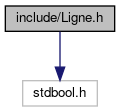
\includegraphics[width=162pt]{Ligne_8h__incl}
\end{center}
\end{figure}
Ce graphe montre quels fichiers incluent directement ou indirectement ce fichier \+:
\nopagebreak
\begin{figure}[H]
\begin{center}
\leavevmode
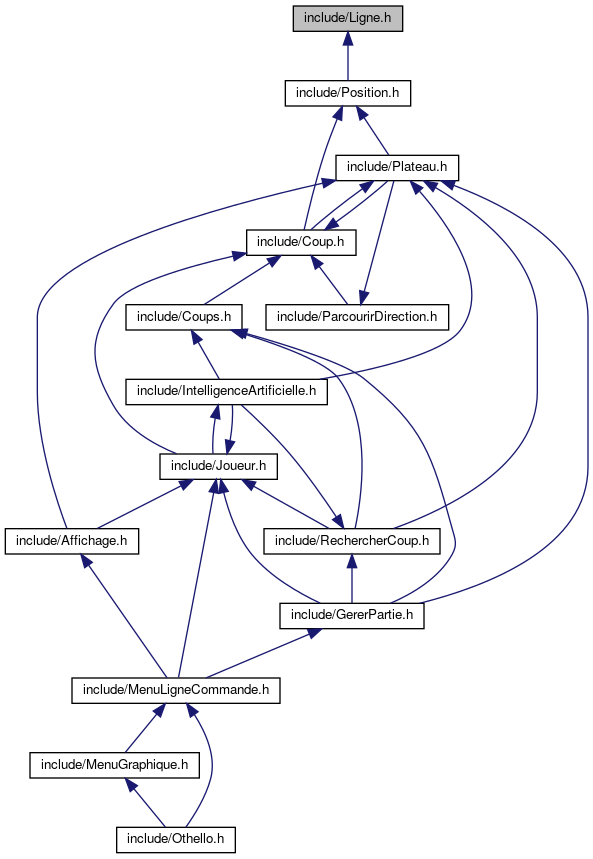
\includegraphics[width=350pt]{Ligne_8h__dep__incl}
\end{center}
\end{figure}
\subsection*{Énumérations}
\begin{DoxyCompactItemize}
\item 
enum \hyperlink{Ligne_8h_a5cdc09714e36ad7319234eab8fdf5e0b}{Ligne} \{ \newline
{\bfseries Un}, 
{\bfseries Deux}, 
{\bfseries Trois}, 
{\bfseries Quatre}, 
\newline
{\bfseries Cinq}, 
{\bfseries Six}, 
{\bfseries Sept}, 
{\bfseries Huit}
 \}\begin{DoxyCompactList}\small\item\em L\textquotesingle{}énumeration permet de travailler avec les Ligne autrement que des integer. \end{DoxyCompactList}
\end{DoxyCompactItemize}
\subsection*{Fonctions}
\begin{DoxyCompactItemize}
\item 
\mbox{\Hypertarget{Ligne_8h_a6d48e750f0ae2e011074d1cccb44cce2}\label{Ligne_8h_a6d48e750f0ae2e011074d1cccb44cce2}} 
\hyperlink{Ligne_8h_a5cdc09714e36ad7319234eab8fdf5e0b}{Ligne} {\bfseries L\+I\+G\+N\+E\+\_\+\+Obtenir\+Ligne\+Depuis\+Int} (int lig\+Num)
\item 
\mbox{\Hypertarget{Ligne_8h_ad5c60f85f6b2861a413ebb447d57b8c6}\label{Ligne_8h_ad5c60f85f6b2861a413ebb447d57b8c6}} 
int {\bfseries L\+I\+G\+N\+E\+\_\+\+Obtenir\+Numero\+Ligne} (\hyperlink{Ligne_8h_a5cdc09714e36ad7319234eab8fdf5e0b}{Ligne} ligne)
\item 
bool \hyperlink{Ligne_8h_a65d9b04da55e610a79cfe9895c743153}{L\+I\+G\+N\+E\+\_\+\+Sont\+Egales\+Lignes} (\hyperlink{Ligne_8h_a5cdc09714e36ad7319234eab8fdf5e0b}{Ligne} ligne1, \hyperlink{Ligne_8h_a5cdc09714e36ad7319234eab8fdf5e0b}{Ligne} ligne2)
\begin{DoxyCompactList}\small\item\em Détermine si deux Ligne sont égales. \end{DoxyCompactList}\end{DoxyCompactItemize}


\subsection{Description détaillée}
Fichier contenant la définition de l\textquotesingle{}enum Ligne et de ses fonctions associées. 



\subsection{Documentation du type de l\textquotesingle{}énumération}
\mbox{\Hypertarget{Ligne_8h_a5cdc09714e36ad7319234eab8fdf5e0b}\label{Ligne_8h_a5cdc09714e36ad7319234eab8fdf5e0b}} 
\index{Ligne.\+h@{Ligne.\+h}!Ligne@{Ligne}}
\index{Ligne@{Ligne}!Ligne.\+h@{Ligne.\+h}}
\subsubsection{\texorpdfstring{Ligne}{Ligne}}
{\footnotesize\ttfamily enum \hyperlink{Ligne_8h_a5cdc09714e36ad7319234eab8fdf5e0b}{Ligne}}



L\textquotesingle{}énumeration permet de travailler avec les Ligne autrement que des integer. 

Le problème étant que les indices et tableaux en C commencent en 0, alors que nos Ligne à nous commencent en 1. 

\subsection{Documentation des fonctions}
\mbox{\Hypertarget{Ligne_8h_a65d9b04da55e610a79cfe9895c743153}\label{Ligne_8h_a65d9b04da55e610a79cfe9895c743153}} 
\index{Ligne.\+h@{Ligne.\+h}!L\+I\+G\+N\+E\+\_\+\+Sont\+Egales\+Lignes@{L\+I\+G\+N\+E\+\_\+\+Sont\+Egales\+Lignes}}
\index{L\+I\+G\+N\+E\+\_\+\+Sont\+Egales\+Lignes@{L\+I\+G\+N\+E\+\_\+\+Sont\+Egales\+Lignes}!Ligne.\+h@{Ligne.\+h}}
\subsubsection{\texorpdfstring{L\+I\+G\+N\+E\+\_\+\+Sont\+Egales\+Lignes()}{LIGNE\_SontEgalesLignes()}}
{\footnotesize\ttfamily bool L\+I\+G\+N\+E\+\_\+\+Sont\+Egales\+Lignes (\begin{DoxyParamCaption}\item[{\hyperlink{Ligne_8h_a5cdc09714e36ad7319234eab8fdf5e0b}{Ligne}}]{ligne1,  }\item[{\hyperlink{Ligne_8h_a5cdc09714e36ad7319234eab8fdf5e0b}{Ligne}}]{ligne2 }\end{DoxyParamCaption})}



Détermine si deux Ligne sont égales. 


\begin{DoxyParams}{Paramètres}
{\em ligne1} & Première Ligne à comparer. \\
\hline
{\em ligne2} & Deuxième Ligne à comparer.\\
\hline
\end{DoxyParams}
\begin{DoxyReturn}{Renvoie}
true si les Ligne sont égales, false sinon. 
\end{DoxyReturn}

\hypertarget{Menu_8h}{}\section{Référence du fichier include/\+Menu.h}
\label{Menu_8h}\index{include/\+Menu.\+h@{include/\+Menu.\+h}}


Fichier contenant la définition les fonctions utilisées par les fichiers Menu\+Graphique et Menu\+Ligne\+Commande.  


{\ttfamily \#include $<$stdlib.\+h$>$}\newline
{\ttfamily \#include $<$string.\+h$>$}\newline
{\ttfamily \#include $<$stdio.\+h$>$}\newline
{\ttfamily \#include \char`\"{}Couleur.\+h\char`\"{}}\newline
Graphe des dépendances par inclusion de Menu.\+h\+:
\nopagebreak
\begin{figure}[H]
\begin{center}
\leavevmode
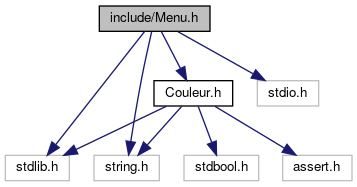
\includegraphics[width=340pt]{Menu_8h__incl}
\end{center}
\end{figure}
Ce graphe montre quels fichiers incluent directement ou indirectement ce fichier \+:
\nopagebreak
\begin{figure}[H]
\begin{center}
\leavevmode
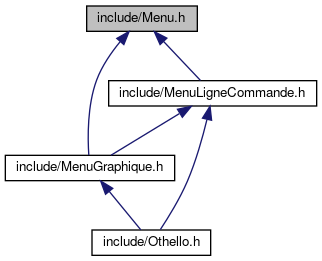
\includegraphics[width=314pt]{Menu_8h__dep__incl}
\end{center}
\end{figure}
\subsection*{Macros}
\begin{DoxyCompactItemize}
\item 
\mbox{\Hypertarget{Menu_8h_af940edd05f0d409818cdbdd8e7dc900d}\label{Menu_8h_af940edd05f0d409818cdbdd8e7dc900d}} 
\#define {\bfseries J\+O\+U\+E\+U\+R\+V\+S\+J\+O\+U\+E\+UR}~\char`\"{}pvp\char`\"{}
\item 
\mbox{\Hypertarget{Menu_8h_ad4359cb228b958251122149b5b911e7b}\label{Menu_8h_ad4359cb228b958251122149b5b911e7b}} 
\#define {\bfseries J\+O\+U\+E\+U\+R\+V\+S\+IA}~\char`\"{}standard\char`\"{}
\item 
\mbox{\Hypertarget{Menu_8h_a7e7fe93f81a69e99ed550c3d7f51fd0e}\label{Menu_8h_a7e7fe93f81a69e99ed550c3d7f51fd0e}} 
\#define {\bfseries I\+A\+V\+S\+IA}~\char`\"{}tournoi\char`\"{}
\item 
\mbox{\Hypertarget{Menu_8h_ae8a798ec5e0449028e485688e8241b5e}\label{Menu_8h_ae8a798ec5e0449028e485688e8241b5e}} 
\#define {\bfseries H\+E\+LP}~\char`\"{}help\char`\"{}
\item 
\mbox{\Hypertarget{Menu_8h_ac11857bfa43dfdfb5c7523cc3b2a4059}\label{Menu_8h_ac11857bfa43dfdfb5c7523cc3b2a4059}} 
\#define {\bfseries P\+R\+O\+F\+O\+N\+D\+E\+U\+R\+\_\+\+D\+E\+F\+A\+U\+T\+\_\+\+IA}~5
\item 
\mbox{\Hypertarget{Menu_8h_a18e566f9f7ca17ca887faf2fe188d458}\label{Menu_8h_a18e566f9f7ca17ca887faf2fe188d458}} 
\#define {\bfseries P\+R\+O\+N\+D\+E\+U\+R\+\_\+\+M\+A\+X\+\_\+\+IA}~100
\end{DoxyCompactItemize}
\subsection*{Fonctions}
\begin{DoxyCompactItemize}
\item 
int \hyperlink{Menu_8h_a8b2641448e9af8b8c33e082c6ce155da}{M\+E\+N\+U\+\_\+\+Obtenir\+Profondeur\+I\+A\+Depuis\+Arguments} (int nb\+Arguments, char $\ast$$\ast$arguments)
\begin{DoxyCompactList}\small\item\em Obtient la profondeur de l\textquotesingle{}IA passée en paramètre ou bien une profondeur par défaut. \end{DoxyCompactList}\item 
int \hyperlink{Menu_8h_afe5946230522e8e55da3abebcf261018}{M\+E\+N\+U\+\_\+\+Saisie\+Integer} (int min, int max)
\begin{DoxyCompactList}\small\item\em Obtient un integer entre deux bornes comprises à partir d\textquotesingle{}une saisie utilisateur. \end{DoxyCompactList}\item 
char $\ast$ \hyperlink{Menu_8h_af4b86d0d6db997cf29dc069bbb1cd7f3}{M\+E\+N\+U\+\_\+\+Obtenir\+String\+Couleur\+Premier\+Joueur\+Depuis\+Arguments} (char $\ast$$\ast$arguments)
\begin{DoxyCompactList}\small\item\em Obtient depuis la liste des arguments du main le String correspondant à la couleur du premier \hyperlink{structJoueur}{Joueur}. \end{DoxyCompactList}\end{DoxyCompactItemize}


\subsection{Description détaillée}
Fichier contenant la définition les fonctions utilisées par les fichiers Menu\+Graphique et Menu\+Ligne\+Commande. 



\subsection{Documentation des fonctions}
\mbox{\Hypertarget{Menu_8h_a8b2641448e9af8b8c33e082c6ce155da}\label{Menu_8h_a8b2641448e9af8b8c33e082c6ce155da}} 
\index{Menu.\+h@{Menu.\+h}!M\+E\+N\+U\+\_\+\+Obtenir\+Profondeur\+I\+A\+Depuis\+Arguments@{M\+E\+N\+U\+\_\+\+Obtenir\+Profondeur\+I\+A\+Depuis\+Arguments}}
\index{M\+E\+N\+U\+\_\+\+Obtenir\+Profondeur\+I\+A\+Depuis\+Arguments@{M\+E\+N\+U\+\_\+\+Obtenir\+Profondeur\+I\+A\+Depuis\+Arguments}!Menu.\+h@{Menu.\+h}}
\subsubsection{\texorpdfstring{M\+E\+N\+U\+\_\+\+Obtenir\+Profondeur\+I\+A\+Depuis\+Arguments()}{MENU\_ObtenirProfondeurIADepuisArguments()}}
{\footnotesize\ttfamily int M\+E\+N\+U\+\_\+\+Obtenir\+Profondeur\+I\+A\+Depuis\+Arguments (\begin{DoxyParamCaption}\item[{int}]{nb\+Arguments,  }\item[{char $\ast$$\ast$}]{arguments }\end{DoxyParamCaption})}



Obtient la profondeur de l\textquotesingle{}IA passée en paramètre ou bien une profondeur par défaut. 


\begin{DoxyParams}{Paramètres}
{\em nb\+Arguments} & Nombre d\textquotesingle{}arguments en entrée du programme. \\
\hline
{\em arguments} & Arguments en entrée du programme.\\
\hline
\end{DoxyParams}
\begin{DoxyReturn}{Renvoie}
Profondeur de l\textquotesingle{}IA obtenue en paramètre. 
\end{DoxyReturn}
\mbox{\Hypertarget{Menu_8h_af4b86d0d6db997cf29dc069bbb1cd7f3}\label{Menu_8h_af4b86d0d6db997cf29dc069bbb1cd7f3}} 
\index{Menu.\+h@{Menu.\+h}!M\+E\+N\+U\+\_\+\+Obtenir\+String\+Couleur\+Premier\+Joueur\+Depuis\+Arguments@{M\+E\+N\+U\+\_\+\+Obtenir\+String\+Couleur\+Premier\+Joueur\+Depuis\+Arguments}}
\index{M\+E\+N\+U\+\_\+\+Obtenir\+String\+Couleur\+Premier\+Joueur\+Depuis\+Arguments@{M\+E\+N\+U\+\_\+\+Obtenir\+String\+Couleur\+Premier\+Joueur\+Depuis\+Arguments}!Menu.\+h@{Menu.\+h}}
\subsubsection{\texorpdfstring{M\+E\+N\+U\+\_\+\+Obtenir\+String\+Couleur\+Premier\+Joueur\+Depuis\+Arguments()}{MENU\_ObtenirStringCouleurPremierJoueurDepuisArguments()}}
{\footnotesize\ttfamily char$\ast$ M\+E\+N\+U\+\_\+\+Obtenir\+String\+Couleur\+Premier\+Joueur\+Depuis\+Arguments (\begin{DoxyParamCaption}\item[{char $\ast$$\ast$}]{arguments }\end{DoxyParamCaption})}



Obtient depuis la liste des arguments du main le String correspondant à la couleur du premier \hyperlink{structJoueur}{Joueur}. 


\begin{DoxyParams}{Paramètres}
{\em arguments} & Arguments en entrée du programme.\\
\hline
\end{DoxyParams}
\begin{DoxyReturn}{Renvoie}
String correspondant au nom d\textquotesingle{}une couleur. 
\end{DoxyReturn}
\mbox{\Hypertarget{Menu_8h_afe5946230522e8e55da3abebcf261018}\label{Menu_8h_afe5946230522e8e55da3abebcf261018}} 
\index{Menu.\+h@{Menu.\+h}!M\+E\+N\+U\+\_\+\+Saisie\+Integer@{M\+E\+N\+U\+\_\+\+Saisie\+Integer}}
\index{M\+E\+N\+U\+\_\+\+Saisie\+Integer@{M\+E\+N\+U\+\_\+\+Saisie\+Integer}!Menu.\+h@{Menu.\+h}}
\subsubsection{\texorpdfstring{M\+E\+N\+U\+\_\+\+Saisie\+Integer()}{MENU\_SaisieInteger()}}
{\footnotesize\ttfamily int M\+E\+N\+U\+\_\+\+Saisie\+Integer (\begin{DoxyParamCaption}\item[{int}]{min,  }\item[{int}]{max }\end{DoxyParamCaption})}



Obtient un integer entre deux bornes comprises à partir d\textquotesingle{}une saisie utilisateur. 


\begin{DoxyParams}{Paramètres}
{\em min} & Borne minimale. \\
\hline
{\em max} & Borne maximale.\\
\hline
\end{DoxyParams}
\begin{DoxyReturn}{Renvoie}
Integer saisi par l\textquotesingle{}utilisateur. 
\end{DoxyReturn}

\hypertarget{MenuGraphique_8h}{}\section{Référence du fichier include/\+Menu\+Graphique.h}
\label{MenuGraphique_8h}\index{include/\+Menu\+Graphique.\+h@{include/\+Menu\+Graphique.\+h}}


Fichier contenant la définition de fonctions permettant d\textquotesingle{}avoir un menu graphique pour lancer le jeu.  


{\ttfamily \#include \char`\"{}Menu.\+h\char`\"{}}\newline
{\ttfamily \#include \char`\"{}Menu\+Ligne\+Commande.\+h\char`\"{}}\newline
Graphe des dépendances par inclusion de Menu\+Graphique.\+h\+:
\nopagebreak
\begin{figure}[H]
\begin{center}
\leavevmode
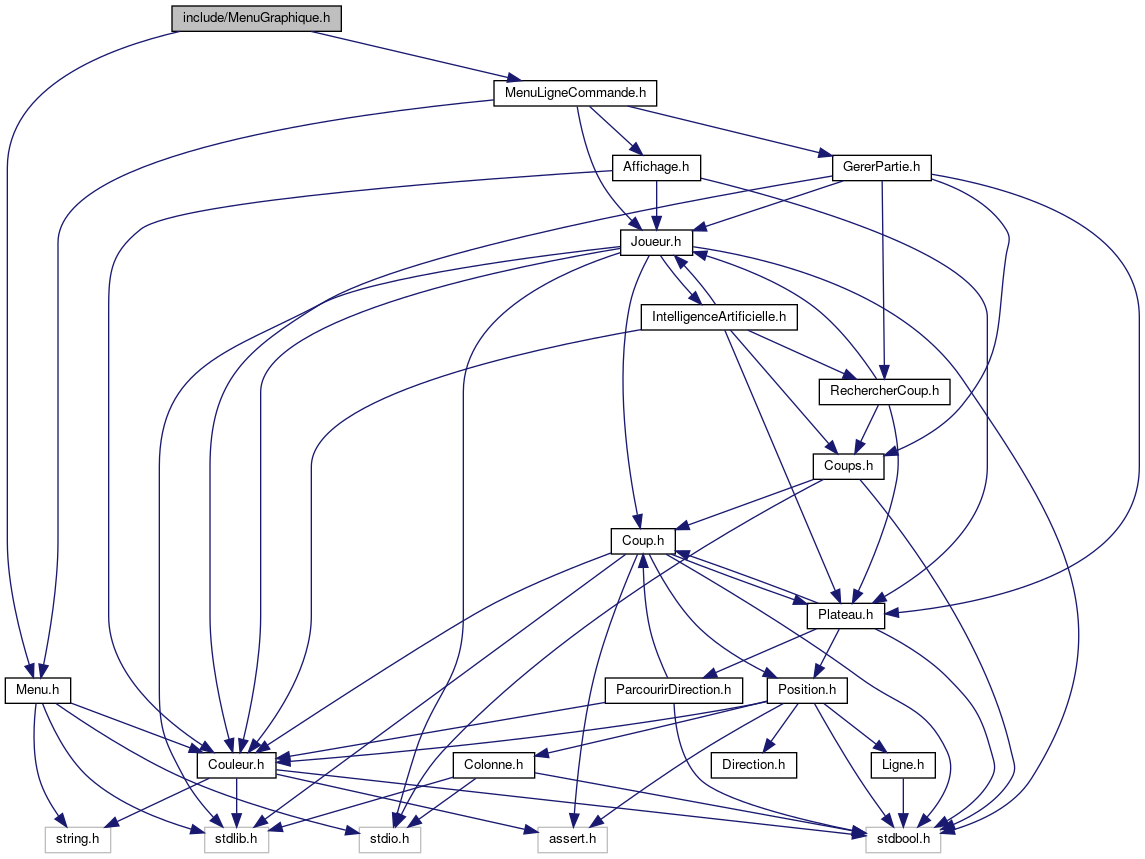
\includegraphics[width=350pt]{MenuGraphique_8h__incl}
\end{center}
\end{figure}
Ce graphe montre quels fichiers incluent directement ou indirectement ce fichier \+:
\nopagebreak
\begin{figure}[H]
\begin{center}
\leavevmode
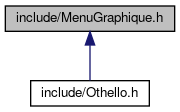
\includegraphics[width=207pt]{MenuGraphique_8h__dep__incl}
\end{center}
\end{figure}
\subsection*{Fonctions}
\begin{DoxyCompactItemize}
\item 
void \hyperlink{MenuGraphique_8h_a28c8c8fade9f041e6d015f86a5b5ffd8}{M\+E\+N\+U\+\_\+\+G\+\_\+\+Menu\+Graphique} ()
\begin{DoxyCompactList}\small\item\em Lance un enchainement de commandes pour lancer les fonctionnalités du jeu. \end{DoxyCompactList}\end{DoxyCompactItemize}


\subsection{Description détaillée}
Fichier contenant la définition de fonctions permettant d\textquotesingle{}avoir un menu graphique pour lancer le jeu. 



\subsection{Documentation des fonctions}
\mbox{\Hypertarget{MenuGraphique_8h_a28c8c8fade9f041e6d015f86a5b5ffd8}\label{MenuGraphique_8h_a28c8c8fade9f041e6d015f86a5b5ffd8}} 
\index{Menu\+Graphique.\+h@{Menu\+Graphique.\+h}!M\+E\+N\+U\+\_\+\+G\+\_\+\+Menu\+Graphique@{M\+E\+N\+U\+\_\+\+G\+\_\+\+Menu\+Graphique}}
\index{M\+E\+N\+U\+\_\+\+G\+\_\+\+Menu\+Graphique@{M\+E\+N\+U\+\_\+\+G\+\_\+\+Menu\+Graphique}!Menu\+Graphique.\+h@{Menu\+Graphique.\+h}}
\subsubsection{\texorpdfstring{M\+E\+N\+U\+\_\+\+G\+\_\+\+Menu\+Graphique()}{MENU\_G\_MenuGraphique()}}
{\footnotesize\ttfamily void M\+E\+N\+U\+\_\+\+G\+\_\+\+Menu\+Graphique (\begin{DoxyParamCaption}{ }\end{DoxyParamCaption})}



Lance un enchainement de commandes pour lancer les fonctionnalités du jeu. 

Il est possible d\textquotesingle{}afficher l\textquotesingle{}aide du jeu ou bien de lancer une partie. Dans le cas où une partie est lancée, le Menu graphique demande d\textquotesingle{}abord dans quel mode de jeu souhaite jouer l\textquotesingle{}utilisateur (P\+VP, standard, tournois).. Il demande ensuite la profondeur de l\textquotesingle{}IA si il y en a une, et la \hyperlink{structCouleur}{Couleur} du premier \hyperlink{structJoueur}{Joueur}. 
\hypertarget{MenuLigneCommande_8h}{}\section{Référence du fichier include/\+Menu\+Ligne\+Commande.h}
\label{MenuLigneCommande_8h}\index{include/\+Menu\+Ligne\+Commande.\+h@{include/\+Menu\+Ligne\+Commande.\+h}}


Fichier contenant la définition de fonctions permettant d\textquotesingle{}avoir un menu en ligne de commande pour lancer le jeu.  


{\ttfamily \#include \char`\"{}Menu.\+h\char`\"{}}\newline
{\ttfamily \#include \char`\"{}Joueur.\+h\char`\"{}}\newline
{\ttfamily \#include \char`\"{}Affichage.\+h\char`\"{}}\newline
{\ttfamily \#include \char`\"{}Gerer\+Partie.\+h\char`\"{}}\newline
Graphe des dépendances par inclusion de Menu\+Ligne\+Commande.\+h\+:
\nopagebreak
\begin{figure}[H]
\begin{center}
\leavevmode
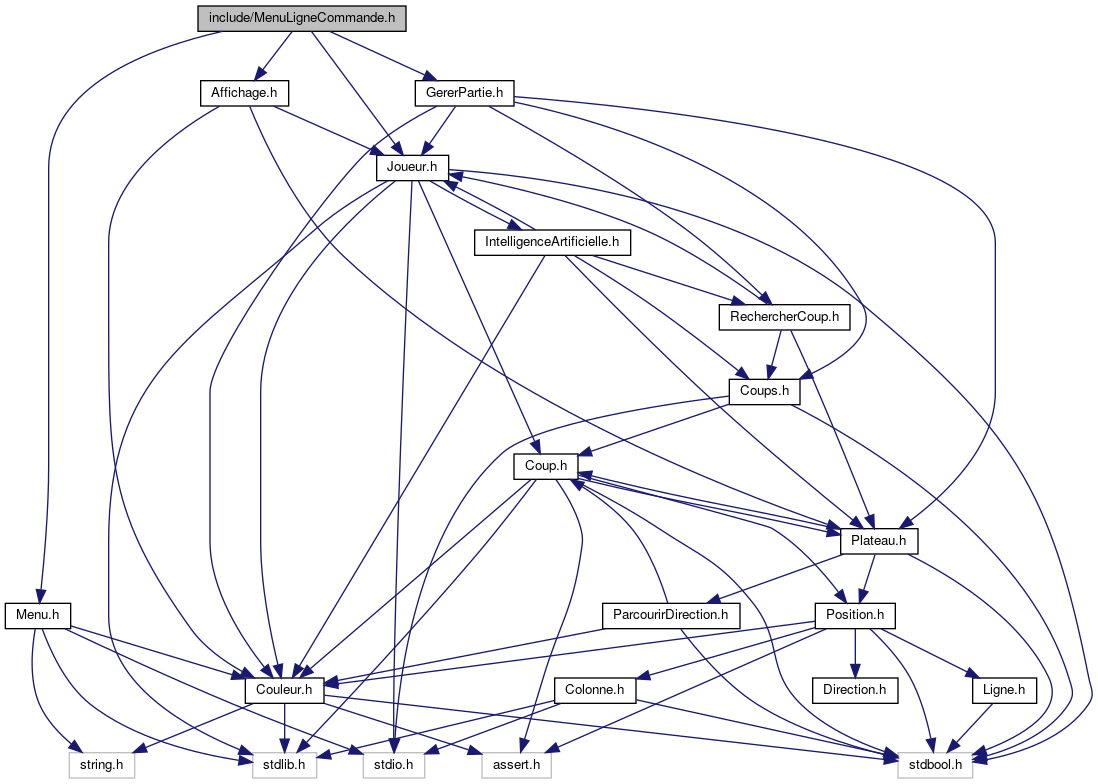
\includegraphics[width=350pt]{MenuLigneCommande_8h__incl}
\end{center}
\end{figure}
Ce graphe montre quels fichiers incluent directement ou indirectement ce fichier \+:
\nopagebreak
\begin{figure}[H]
\begin{center}
\leavevmode
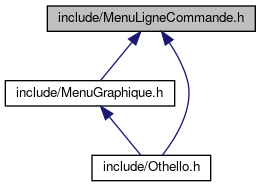
\includegraphics[width=268pt]{MenuLigneCommande_8h__dep__incl}
\end{center}
\end{figure}
\subsection*{Fonctions}
\begin{DoxyCompactItemize}
\item 
void \hyperlink{MenuLigneCommande_8h_a643a35cacd4a3a386ced30ff0af6d0fb}{M\+E\+N\+U\+\_\+\+L\+C\+\_\+\+Menu\+Ligne\+Commande} (int nb\+Arguments, char $\ast$$\ast$arguments)
\begin{DoxyCompactList}\small\item\em Traite les arguments en entrée du programme. \end{DoxyCompactList}\end{DoxyCompactItemize}


\subsection{Description détaillée}
Fichier contenant la définition de fonctions permettant d\textquotesingle{}avoir un menu en ligne de commande pour lancer le jeu. 



\subsection{Documentation des fonctions}
\mbox{\Hypertarget{MenuLigneCommande_8h_a643a35cacd4a3a386ced30ff0af6d0fb}\label{MenuLigneCommande_8h_a643a35cacd4a3a386ced30ff0af6d0fb}} 
\index{Menu\+Ligne\+Commande.\+h@{Menu\+Ligne\+Commande.\+h}!M\+E\+N\+U\+\_\+\+L\+C\+\_\+\+Menu\+Ligne\+Commande@{M\+E\+N\+U\+\_\+\+L\+C\+\_\+\+Menu\+Ligne\+Commande}}
\index{M\+E\+N\+U\+\_\+\+L\+C\+\_\+\+Menu\+Ligne\+Commande@{M\+E\+N\+U\+\_\+\+L\+C\+\_\+\+Menu\+Ligne\+Commande}!Menu\+Ligne\+Commande.\+h@{Menu\+Ligne\+Commande.\+h}}
\subsubsection{\texorpdfstring{M\+E\+N\+U\+\_\+\+L\+C\+\_\+\+Menu\+Ligne\+Commande()}{MENU\_LC\_MenuLigneCommande()}}
{\footnotesize\ttfamily void M\+E\+N\+U\+\_\+\+L\+C\+\_\+\+Menu\+Ligne\+Commande (\begin{DoxyParamCaption}\item[{int}]{nb\+Arguments,  }\item[{char $\ast$$\ast$}]{arguments }\end{DoxyParamCaption})}



Traite les arguments en entrée du programme. 

A partir de ces arguments la fonction va extraire les paramètres utiles au lancement d\textquotesingle{}une partie ou d\textquotesingle{}autres fonctionnalités comme l\textquotesingle{}affichage de l\textquotesingle{}aide. Pour lancer la partie il faut lancer le programme avec le mode de jeu souhaité (standard, pvp, tournois), puis la couleur du premier \hyperlink{structJoueur}{Joueur}, et finalement (optionnellement) un integer correspondant à la profondeur de l\textquotesingle{}IA.


\begin{DoxyParams}{Paramètres}
{\em nb\+Arguments} & Nombre d\textquotesingle{}arguments en entrée du programme. \\
\hline
{\em arguments} & Arguments en entrée du programme. \\
\hline
\end{DoxyParams}

\hypertarget{Othello_8h}{}\section{Référence du fichier include/\+Othello.h}
\label{Othello_8h}\index{include/\+Othello.\+h@{include/\+Othello.\+h}}


Fichier contenant la définition du main du programme.  


{\ttfamily \#include $<$stdio.\+h$>$}\newline
{\ttfamily \#include \char`\"{}Menu\+Graphique.\+h\char`\"{}}\newline
{\ttfamily \#include \char`\"{}Menu\+Ligne\+Commande.\+h\char`\"{}}\newline
Graphe des dépendances par inclusion de Othello.\+h\+:
\nopagebreak
\begin{figure}[H]
\begin{center}
\leavevmode
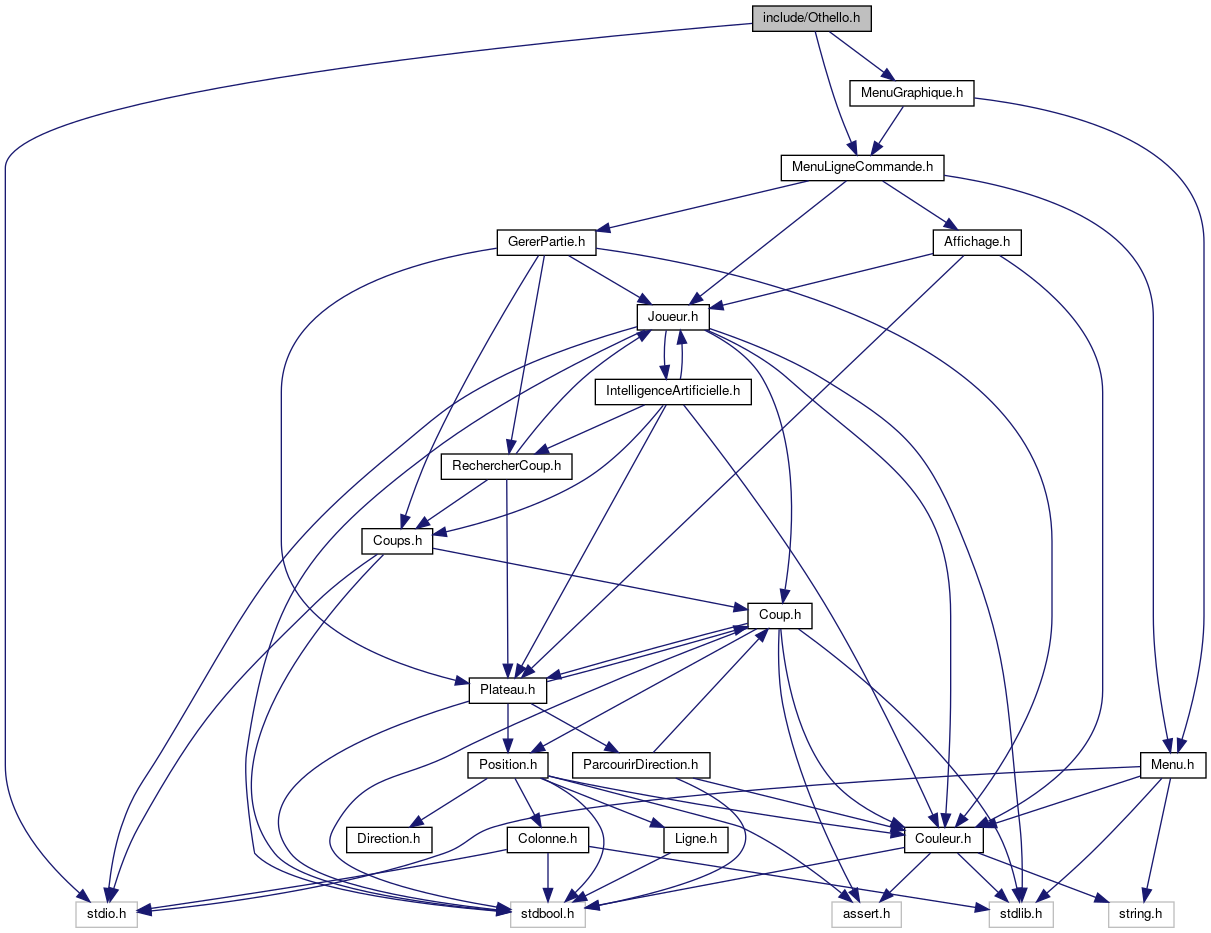
\includegraphics[width=350pt]{Othello_8h__incl}
\end{center}
\end{figure}
\subsection*{Fonctions}
\begin{DoxyCompactItemize}
\item 
int \hyperlink{Othello_8h_a988772f36bad88a3f7900889b591914a}{main} (int nb\+Arguments, char $\ast$$\ast$arguments)
\begin{DoxyCompactList}\small\item\em Entrée du programme. \end{DoxyCompactList}\end{DoxyCompactItemize}


\subsection{Description détaillée}
Fichier contenant la définition du main du programme. 

Il permet de lancer le jeu Othello. 

\subsection{Documentation des fonctions}
\mbox{\Hypertarget{Othello_8h_a988772f36bad88a3f7900889b591914a}\label{Othello_8h_a988772f36bad88a3f7900889b591914a}} 
\index{Othello.\+h@{Othello.\+h}!main@{main}}
\index{main@{main}!Othello.\+h@{Othello.\+h}}
\subsubsection{\texorpdfstring{main()}{main()}}
{\footnotesize\ttfamily int main (\begin{DoxyParamCaption}\item[{int}]{nb\+Arguments,  }\item[{char $\ast$$\ast$}]{arguments }\end{DoxyParamCaption})}



Entrée du programme. 

Elle permet de lancer le jeu Othello.


\begin{DoxyParams}{Paramètres}
{\em nb\+Arguments} & Nombre d\textquotesingle{}arguments en entrée du programme. \\
\hline
{\em arguments} & Les arguments en entrée du programme.\\
\hline
\end{DoxyParams}
\begin{DoxyReturn}{Renvoie}
E\+X\+I\+T\+\_\+\+S\+U\+C\+C\+E\+SS -\/ Arrêt normal du programme. 
\end{DoxyReturn}

\hypertarget{ParcourirDirection_8h}{}\section{Référence du fichier include/\+Parcourir\+Direction.h}
\label{ParcourirDirection_8h}\index{include/\+Parcourir\+Direction.\+h@{include/\+Parcourir\+Direction.\+h}}


Fichier contenant la définition de fonctions pour parcourir un plateau dans des directions données et voir si un coup est possible.  


{\ttfamily \#include $<$stdbool.\+h$>$}\newline
{\ttfamily \#include \char`\"{}Couleur.\+h\char`\"{}}\newline
{\ttfamily \#include \char`\"{}Coup.\+h\char`\"{}}\newline
Graphe des dépendances par inclusion de Parcourir\+Direction.\+h\+:
\nopagebreak
\begin{figure}[H]
\begin{center}
\leavevmode
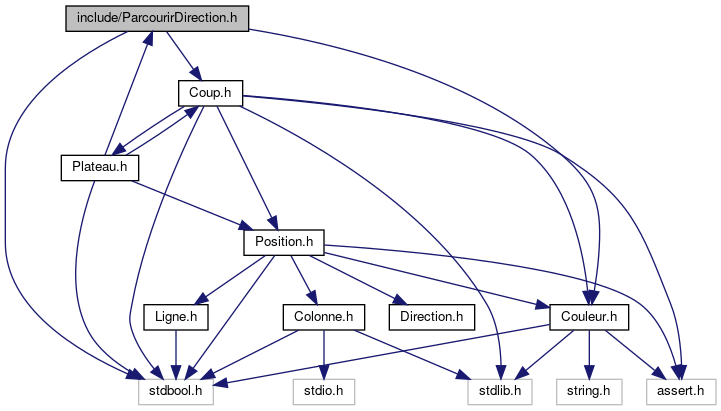
\includegraphics[width=350pt]{ParcourirDirection_8h__incl}
\end{center}
\end{figure}
Ce graphe montre quels fichiers incluent directement ou indirectement ce fichier \+:
\nopagebreak
\begin{figure}[H]
\begin{center}
\leavevmode
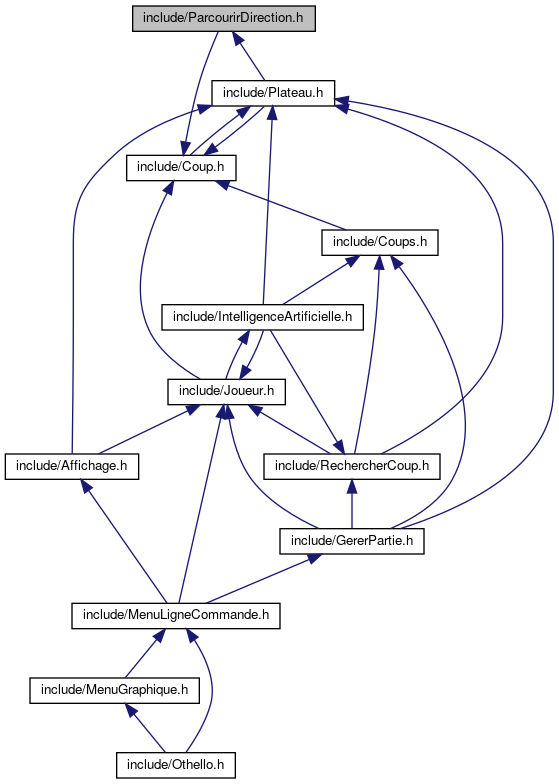
\includegraphics[width=350pt]{ParcourirDirection_8h__dep__incl}
\end{center}
\end{figure}
\subsection*{Fonctions}
\begin{DoxyCompactItemize}
\item 
bool \hyperlink{ParcourirDirection_8h_adff04d0a50f7374e644ab91b9a653dd0}{R\+E\+C\+H\+E\+R\+C\+H\+E\+D\+I\+R\+E\+C\+T\+I\+O\+N\+S\+\_\+\+Coup\+Possible\+Dans\+Une\+Direction\+Quelconque} (\hyperlink{structCouleur}{Couleur} $\ast$plateau, \hyperlink{structCoup}{Coup} coup)
\begin{DoxyCompactList}\small\item\em Détermine si un \hyperlink{structCoup}{Coup} permet de capturer des pions dans au moins une Direction. \end{DoxyCompactList}\item 
bool \hyperlink{ParcourirDirection_8h_ac6935ce8b96af10a9ac50c1a286f0752}{R\+E\+C\+H\+E\+R\+C\+H\+E\+D\+I\+R\+E\+C\+T\+I\+O\+N\+S\+\_\+\+Coup\+Possible\+Dans\+Direction} (\hyperlink{structCouleur}{Couleur} $\ast$plateau, \hyperlink{structCoup}{Coup} coup, \hyperlink{Direction_8h_a224b9163917ac32fc95a60d8c1eec3aa}{Direction} direction)
\begin{DoxyCompactList}\small\item\em Détermine si un \hyperlink{structCoup}{Coup} permet de capturer des pions dans une Direction donnée. \end{DoxyCompactList}\end{DoxyCompactItemize}


\subsection{Description détaillée}
Fichier contenant la définition de fonctions pour parcourir un plateau dans des directions données et voir si un coup est possible. 



\subsection{Documentation des fonctions}
\mbox{\Hypertarget{ParcourirDirection_8h_ac6935ce8b96af10a9ac50c1a286f0752}\label{ParcourirDirection_8h_ac6935ce8b96af10a9ac50c1a286f0752}} 
\index{Parcourir\+Direction.\+h@{Parcourir\+Direction.\+h}!R\+E\+C\+H\+E\+R\+C\+H\+E\+D\+I\+R\+E\+C\+T\+I\+O\+N\+S\+\_\+\+Coup\+Possible\+Dans\+Direction@{R\+E\+C\+H\+E\+R\+C\+H\+E\+D\+I\+R\+E\+C\+T\+I\+O\+N\+S\+\_\+\+Coup\+Possible\+Dans\+Direction}}
\index{R\+E\+C\+H\+E\+R\+C\+H\+E\+D\+I\+R\+E\+C\+T\+I\+O\+N\+S\+\_\+\+Coup\+Possible\+Dans\+Direction@{R\+E\+C\+H\+E\+R\+C\+H\+E\+D\+I\+R\+E\+C\+T\+I\+O\+N\+S\+\_\+\+Coup\+Possible\+Dans\+Direction}!Parcourir\+Direction.\+h@{Parcourir\+Direction.\+h}}
\subsubsection{\texorpdfstring{R\+E\+C\+H\+E\+R\+C\+H\+E\+D\+I\+R\+E\+C\+T\+I\+O\+N\+S\+\_\+\+Coup\+Possible\+Dans\+Direction()}{RECHERCHEDIRECTIONS\_CoupPossibleDansDirection()}}
{\footnotesize\ttfamily bool R\+E\+C\+H\+E\+R\+C\+H\+E\+D\+I\+R\+E\+C\+T\+I\+O\+N\+S\+\_\+\+Coup\+Possible\+Dans\+Direction (\begin{DoxyParamCaption}\item[{\hyperlink{structCouleur}{Couleur} $\ast$}]{plateau,  }\item[{\hyperlink{structCoup}{Coup}}]{coup,  }\item[{\hyperlink{Direction_8h_a224b9163917ac32fc95a60d8c1eec3aa}{Direction}}]{direction }\end{DoxyParamCaption})}



Détermine si un \hyperlink{structCoup}{Coup} permet de capturer des pions dans une Direction donnée. 


\begin{DoxyParams}{Paramètres}
{\em plateau\+De\+Jeu} & Plateau de jeu. \\
\hline
{\em coup} & \hyperlink{structCoup}{Coup} dont on souhaite déterminer l\textquotesingle{}influence sur le plateau. \\
\hline
{\em direction} & Direction dans laquelle on recherche la capture potentielle de pions.\\
\hline
\end{DoxyParams}
\begin{DoxyReturn}{Renvoie}
true si le \hyperlink{structCoup}{Coup} permet la capture de pions, false sinon. 
\end{DoxyReturn}
\mbox{\Hypertarget{ParcourirDirection_8h_adff04d0a50f7374e644ab91b9a653dd0}\label{ParcourirDirection_8h_adff04d0a50f7374e644ab91b9a653dd0}} 
\index{Parcourir\+Direction.\+h@{Parcourir\+Direction.\+h}!R\+E\+C\+H\+E\+R\+C\+H\+E\+D\+I\+R\+E\+C\+T\+I\+O\+N\+S\+\_\+\+Coup\+Possible\+Dans\+Une\+Direction\+Quelconque@{R\+E\+C\+H\+E\+R\+C\+H\+E\+D\+I\+R\+E\+C\+T\+I\+O\+N\+S\+\_\+\+Coup\+Possible\+Dans\+Une\+Direction\+Quelconque}}
\index{R\+E\+C\+H\+E\+R\+C\+H\+E\+D\+I\+R\+E\+C\+T\+I\+O\+N\+S\+\_\+\+Coup\+Possible\+Dans\+Une\+Direction\+Quelconque@{R\+E\+C\+H\+E\+R\+C\+H\+E\+D\+I\+R\+E\+C\+T\+I\+O\+N\+S\+\_\+\+Coup\+Possible\+Dans\+Une\+Direction\+Quelconque}!Parcourir\+Direction.\+h@{Parcourir\+Direction.\+h}}
\subsubsection{\texorpdfstring{R\+E\+C\+H\+E\+R\+C\+H\+E\+D\+I\+R\+E\+C\+T\+I\+O\+N\+S\+\_\+\+Coup\+Possible\+Dans\+Une\+Direction\+Quelconque()}{RECHERCHEDIRECTIONS\_CoupPossibleDansUneDirectionQuelconque()}}
{\footnotesize\ttfamily bool R\+E\+C\+H\+E\+R\+C\+H\+E\+D\+I\+R\+E\+C\+T\+I\+O\+N\+S\+\_\+\+Coup\+Possible\+Dans\+Une\+Direction\+Quelconque (\begin{DoxyParamCaption}\item[{\hyperlink{structCouleur}{Couleur} $\ast$}]{plateau,  }\item[{\hyperlink{structCoup}{Coup}}]{coup }\end{DoxyParamCaption})}



Détermine si un \hyperlink{structCoup}{Coup} permet de capturer des pions dans au moins une Direction. 


\begin{DoxyParams}{Paramètres}
{\em plateau\+De\+Jeu} & Plateau de jeu. \\
\hline
{\em coup} & \hyperlink{structCoup}{Coup} dont on souhaite déterminer l\textquotesingle{}influence sur le plateau.\\
\hline
\end{DoxyParams}
\begin{DoxyReturn}{Renvoie}
true si le \hyperlink{structCoup}{Coup} permet la capture de pions, false sinon. 
\end{DoxyReturn}

\hypertarget{Plateau_8h}{}\section{Référence du fichier include/\+Plateau.h}
\label{Plateau_8h}\index{include/\+Plateau.\+h@{include/\+Plateau.\+h}}


Fichier contenant la définition des fonctions permettant d\textquotesingle{}intéragir avec le plateau de jeu.  


{\ttfamily \#include $<$stdbool.\+h$>$}\newline
{\ttfamily \#include \char`\"{}Position.\+h\char`\"{}}\newline
{\ttfamily \#include \char`\"{}Coup.\+h\char`\"{}}\newline
{\ttfamily \#include \char`\"{}Parcourir\+Direction.\+h\char`\"{}}\newline
Graphe des dépendances par inclusion de Plateau.\+h\+:
\nopagebreak
\begin{figure}[H]
\begin{center}
\leavevmode
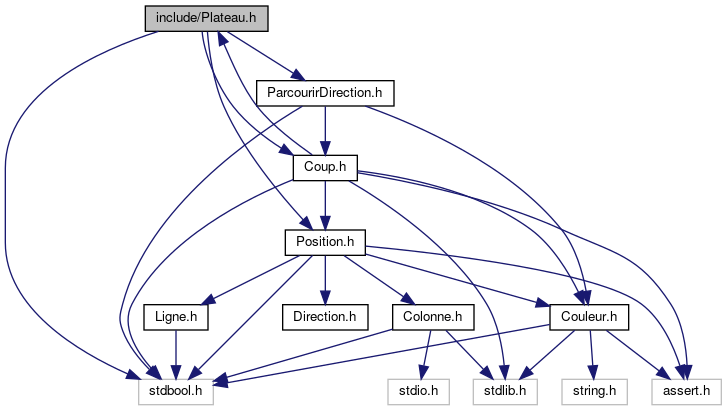
\includegraphics[width=350pt]{Plateau_8h__incl}
\end{center}
\end{figure}
Ce graphe montre quels fichiers incluent directement ou indirectement ce fichier \+:
\nopagebreak
\begin{figure}[H]
\begin{center}
\leavevmode
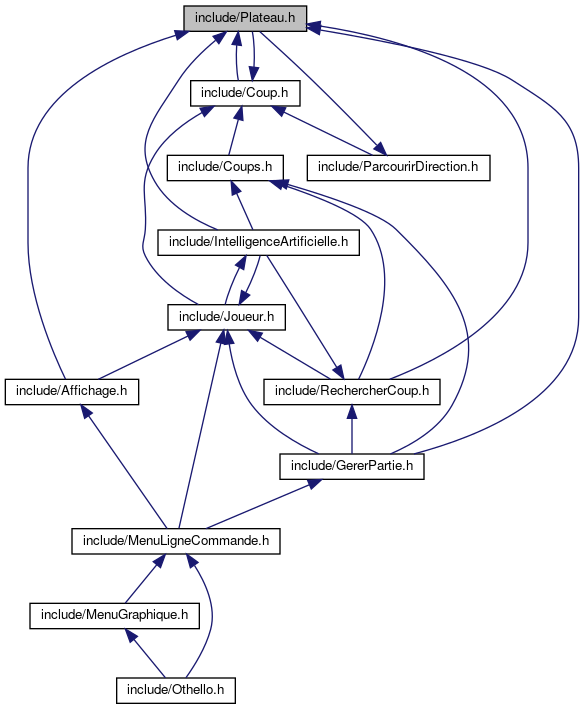
\includegraphics[width=350pt]{Plateau_8h__dep__incl}
\end{center}
\end{figure}
\subsection*{Macros}
\begin{DoxyCompactItemize}
\item 
\mbox{\Hypertarget{Plateau_8h_a7b29335add3a553ed85d0e3ace85629c}\label{Plateau_8h_a7b29335add3a553ed85d0e3ace85629c}} 
\#define {\bfseries T\+A\+I\+L\+LE}~8
\end{DoxyCompactItemize}
\subsection*{Fonctions}
\begin{DoxyCompactItemize}
\item 
\mbox{\Hypertarget{Plateau_8h_a16ae8e251080137fd93da6d2f6b761bc}\label{Plateau_8h_a16ae8e251080137fd93da6d2f6b761bc}} 
void {\bfseries P\+L\+A\+T\+E\+A\+U\+\_\+\+Initialiser\+Plateau} (\hyperlink{structCouleur}{Couleur} $\ast$plateau)
\item 
\hyperlink{structCouleur}{Couleur} $\ast$ \hyperlink{Plateau_8h_ad1972b1f8f2087b03bca55805a2a0a73}{P\+L\+A\+T\+E\+A\+U\+\_\+\+Creer\+Plateau} ()
\begin{DoxyCompactList}\small\item\em Crée un plateau. \end{DoxyCompactList}\item 
void \hyperlink{Plateau_8h_a527bd475dd6c51db8b640f3ccca0d75a}{P\+L\+A\+T\+E\+A\+U\+\_\+\+Jouer\+Coup} (\hyperlink{structCouleur}{Couleur} $\ast$plateau, \hyperlink{structCoup}{Coup} coup)
\begin{DoxyCompactList}\small\item\em Joue un coup sur le plateau. \end{DoxyCompactList}\item 
\hyperlink{structCouleur}{Couleur} \hyperlink{Plateau_8h_afce75f28d97af92ab6ccfc22a6c10cf5}{P\+L\+A\+T\+E\+A\+U\+\_\+\+Obtenir\+Couleur\+Avec\+Position} (\hyperlink{structCouleur}{Couleur} $\ast$plateau, \hyperlink{structPosition}{Position} position)
\begin{DoxyCompactList}\small\item\em Permet d\textquotesingle{}obtenir la \hyperlink{structCouleur}{Couleur} présente sur le plateau grâce à une \hyperlink{structPosition}{Position}. \end{DoxyCompactList}\item 
bool \hyperlink{Plateau_8h_a29307bcab64380a2d5815867ca965552}{P\+L\+A\+T\+E\+A\+U\+\_\+\+Est\+Position\+Libre} (\hyperlink{structCouleur}{Couleur} $\ast$plateau, \hyperlink{structPosition}{Position} position)
\begin{DoxyCompactList}\small\item\em Détermine si la \hyperlink{structPosition}{Position} est libre à la \hyperlink{structPosition}{Position} donnée. \end{DoxyCompactList}\item 
int \hyperlink{Plateau_8h_a41bf1a2697e9d8891d919f307f0881c1}{P\+L\+A\+T\+E\+A\+U\+\_\+\+Obtenir\+Taille} (\hyperlink{structCouleur}{Couleur} $\ast$plateau)
\begin{DoxyCompactList}\small\item\em Permet d\textquotesingle{}obtenir la taille d\textquotesingle{}un plateau. \end{DoxyCompactList}\item 
bool \hyperlink{Plateau_8h_a93ebca467b0af23b97f559d54323b7a2}{P\+L\+A\+T\+E\+A\+U\+\_\+\+Est\+Rempli} (\hyperlink{structCouleur}{Couleur} $\ast$plateau)
\begin{DoxyCompactList}\small\item\em Détermine si le plateau est entièrement rempli. \end{DoxyCompactList}\item 
int \hyperlink{Plateau_8h_a649c5ed91fceb626ebeab35d0b334be9}{P\+L\+A\+T\+E\+A\+U\+\_\+\+Calculer\+Points} (\hyperlink{structCouleur}{Couleur} $\ast$plateau, \hyperlink{structCouleur}{Couleur} couleur)
\begin{DoxyCompactList}\small\item\em Calcule le nombre de points d\textquotesingle{}une \hyperlink{structCouleur}{Couleur}. \end{DoxyCompactList}\item 
bool \hyperlink{Plateau_8h_a9c2b70ecfa0b94e04ca251af0686b26d}{P\+L\+A\+T\+E\+A\+U\+\_\+\+Est\+Position\+Valide} (\hyperlink{structCouleur}{Couleur} $\ast$plateau, \hyperlink{structPosition}{Position} position)
\begin{DoxyCompactList}\small\item\em Détermine si une \hyperlink{structPosition}{Position} est valide. \end{DoxyCompactList}\item 
void \hyperlink{Plateau_8h_a97260b37600a04f94e722a3cc02c51dc}{P\+L\+A\+T\+E\+A\+U\+\_\+\+Capturer\+Pions} (\hyperlink{structCouleur}{Couleur} $\ast$plateau, \hyperlink{structCoup}{Coup} coup)
\begin{DoxyCompactList}\small\item\em Capture les pions adverses depuis la \hyperlink{structPosition}{Position} d\textquotesingle{}un \hyperlink{structCoup}{Coup} donné. \end{DoxyCompactList}\item 
void \hyperlink{Plateau_8h_a4680e3c7bbc9813fa691122ad41b1ccc}{P\+L\+A\+T\+E\+A\+U\+\_\+\+Capturer\+Pions\+Dans\+Direction} (\hyperlink{structCouleur}{Couleur} $\ast$plateau, \hyperlink{structCoup}{Coup} coup, \hyperlink{Direction_8h_a224b9163917ac32fc95a60d8c1eec3aa}{Direction} direction)
\begin{DoxyCompactList}\small\item\em Capture les pions adverses depuis la \hyperlink{structPosition}{Position} d\textquotesingle{}un \hyperlink{structCoup}{Coup} donné dans une certaine Direction. \end{DoxyCompactList}\end{DoxyCompactItemize}


\subsection{Description détaillée}
Fichier contenant la définition des fonctions permettant d\textquotesingle{}intéragir avec le plateau de jeu. 



\subsection{Documentation des fonctions}
\mbox{\Hypertarget{Plateau_8h_a649c5ed91fceb626ebeab35d0b334be9}\label{Plateau_8h_a649c5ed91fceb626ebeab35d0b334be9}} 
\index{Plateau.\+h@{Plateau.\+h}!P\+L\+A\+T\+E\+A\+U\+\_\+\+Calculer\+Points@{P\+L\+A\+T\+E\+A\+U\+\_\+\+Calculer\+Points}}
\index{P\+L\+A\+T\+E\+A\+U\+\_\+\+Calculer\+Points@{P\+L\+A\+T\+E\+A\+U\+\_\+\+Calculer\+Points}!Plateau.\+h@{Plateau.\+h}}
\subsubsection{\texorpdfstring{P\+L\+A\+T\+E\+A\+U\+\_\+\+Calculer\+Points()}{PLATEAU\_CalculerPoints()}}
{\footnotesize\ttfamily int P\+L\+A\+T\+E\+A\+U\+\_\+\+Calculer\+Points (\begin{DoxyParamCaption}\item[{\hyperlink{structCouleur}{Couleur} $\ast$}]{plateau,  }\item[{\hyperlink{structCouleur}{Couleur}}]{couleur }\end{DoxyParamCaption})}



Calcule le nombre de points d\textquotesingle{}une \hyperlink{structCouleur}{Couleur}. 

Un point équivaut à un pion présent sur le plateau de la couleur donnée.


\begin{DoxyParams}{Paramètres}
{\em plateau} & Plateau de jeu. \\
\hline
{\em couleur} & \hyperlink{structCouleur}{Couleur} dont on souhaite calculer le nombre de points.\\
\hline
\end{DoxyParams}
\begin{DoxyReturn}{Renvoie}
Integer donnant le nombre de points de la \hyperlink{structCouleur}{Couleur} donnée. 
\end{DoxyReturn}
\mbox{\Hypertarget{Plateau_8h_a97260b37600a04f94e722a3cc02c51dc}\label{Plateau_8h_a97260b37600a04f94e722a3cc02c51dc}} 
\index{Plateau.\+h@{Plateau.\+h}!P\+L\+A\+T\+E\+A\+U\+\_\+\+Capturer\+Pions@{P\+L\+A\+T\+E\+A\+U\+\_\+\+Capturer\+Pions}}
\index{P\+L\+A\+T\+E\+A\+U\+\_\+\+Capturer\+Pions@{P\+L\+A\+T\+E\+A\+U\+\_\+\+Capturer\+Pions}!Plateau.\+h@{Plateau.\+h}}
\subsubsection{\texorpdfstring{P\+L\+A\+T\+E\+A\+U\+\_\+\+Capturer\+Pions()}{PLATEAU\_CapturerPions()}}
{\footnotesize\ttfamily void P\+L\+A\+T\+E\+A\+U\+\_\+\+Capturer\+Pions (\begin{DoxyParamCaption}\item[{\hyperlink{structCouleur}{Couleur} $\ast$}]{plateau,  }\item[{\hyperlink{structCoup}{Coup}}]{coup }\end{DoxyParamCaption})}



Capture les pions adverses depuis la \hyperlink{structPosition}{Position} d\textquotesingle{}un \hyperlink{structCoup}{Coup} donné. 

On entend par capture le fait de remplacer la \hyperlink{structCouleur}{Couleur} des pions qui ne sont pas de la \hyperlink{structCouleur}{Couleur} du \hyperlink{structCoup}{Coup} joué par la \hyperlink{structCouleur}{Couleur} de ce dernier. Il est possible de capturer dans les 8 Direction différentes. La capture s\textquotesingle{}arrête dans une Direction quand on rencontre une case avec la même \hyperlink{structCouleur}{Couleur} que celle du \hyperlink{structCoup}{Coup}.


\begin{DoxyParams}{Paramètres}
{\em plateau} & Plateau de jeu. \\
\hline
{\em coup} & \hyperlink{structCoup}{Coup} qui engendre la capture. \\
\hline
\end{DoxyParams}
\mbox{\Hypertarget{Plateau_8h_a4680e3c7bbc9813fa691122ad41b1ccc}\label{Plateau_8h_a4680e3c7bbc9813fa691122ad41b1ccc}} 
\index{Plateau.\+h@{Plateau.\+h}!P\+L\+A\+T\+E\+A\+U\+\_\+\+Capturer\+Pions\+Dans\+Direction@{P\+L\+A\+T\+E\+A\+U\+\_\+\+Capturer\+Pions\+Dans\+Direction}}
\index{P\+L\+A\+T\+E\+A\+U\+\_\+\+Capturer\+Pions\+Dans\+Direction@{P\+L\+A\+T\+E\+A\+U\+\_\+\+Capturer\+Pions\+Dans\+Direction}!Plateau.\+h@{Plateau.\+h}}
\subsubsection{\texorpdfstring{P\+L\+A\+T\+E\+A\+U\+\_\+\+Capturer\+Pions\+Dans\+Direction()}{PLATEAU\_CapturerPionsDansDirection()}}
{\footnotesize\ttfamily void P\+L\+A\+T\+E\+A\+U\+\_\+\+Capturer\+Pions\+Dans\+Direction (\begin{DoxyParamCaption}\item[{\hyperlink{structCouleur}{Couleur} $\ast$}]{plateau,  }\item[{\hyperlink{structCoup}{Coup}}]{coup,  }\item[{\hyperlink{Direction_8h_a224b9163917ac32fc95a60d8c1eec3aa}{Direction}}]{direction }\end{DoxyParamCaption})}



Capture les pions adverses depuis la \hyperlink{structPosition}{Position} d\textquotesingle{}un \hyperlink{structCoup}{Coup} donné dans une certaine Direction. 

cf P\+L\+A\+T\+E\+A\+U\+\_\+\+Capturer\+Pions pour avoir des informations sur la capture.


\begin{DoxyParams}{Paramètres}
{\em plateau} & Plateau de jeu. \\
\hline
{\em coup} & \hyperlink{structCoup}{Coup} qui egendre la capture. \\
\hline
\end{DoxyParams}
\mbox{\Hypertarget{Plateau_8h_ad1972b1f8f2087b03bca55805a2a0a73}\label{Plateau_8h_ad1972b1f8f2087b03bca55805a2a0a73}} 
\index{Plateau.\+h@{Plateau.\+h}!P\+L\+A\+T\+E\+A\+U\+\_\+\+Creer\+Plateau@{P\+L\+A\+T\+E\+A\+U\+\_\+\+Creer\+Plateau}}
\index{P\+L\+A\+T\+E\+A\+U\+\_\+\+Creer\+Plateau@{P\+L\+A\+T\+E\+A\+U\+\_\+\+Creer\+Plateau}!Plateau.\+h@{Plateau.\+h}}
\subsubsection{\texorpdfstring{P\+L\+A\+T\+E\+A\+U\+\_\+\+Creer\+Plateau()}{PLATEAU\_CreerPlateau()}}
{\footnotesize\ttfamily \hyperlink{structCouleur}{Couleur}$\ast$ P\+L\+A\+T\+E\+A\+U\+\_\+\+Creer\+Plateau (\begin{DoxyParamCaption}{ }\end{DoxyParamCaption})}



Crée un plateau. 

\begin{DoxyReturn}{Renvoie}
\+: Pointeur vers un tableau de \hyperlink{structCouleur}{Couleur}, alloué dynamiquement. 
\end{DoxyReturn}
\mbox{\Hypertarget{Plateau_8h_a29307bcab64380a2d5815867ca965552}\label{Plateau_8h_a29307bcab64380a2d5815867ca965552}} 
\index{Plateau.\+h@{Plateau.\+h}!P\+L\+A\+T\+E\+A\+U\+\_\+\+Est\+Position\+Libre@{P\+L\+A\+T\+E\+A\+U\+\_\+\+Est\+Position\+Libre}}
\index{P\+L\+A\+T\+E\+A\+U\+\_\+\+Est\+Position\+Libre@{P\+L\+A\+T\+E\+A\+U\+\_\+\+Est\+Position\+Libre}!Plateau.\+h@{Plateau.\+h}}
\subsubsection{\texorpdfstring{P\+L\+A\+T\+E\+A\+U\+\_\+\+Est\+Position\+Libre()}{PLATEAU\_EstPositionLibre()}}
{\footnotesize\ttfamily bool P\+L\+A\+T\+E\+A\+U\+\_\+\+Est\+Position\+Libre (\begin{DoxyParamCaption}\item[{\hyperlink{structCouleur}{Couleur} $\ast$}]{plateau,  }\item[{\hyperlink{structPosition}{Position}}]{position }\end{DoxyParamCaption})}



Détermine si la \hyperlink{structPosition}{Position} est libre à la \hyperlink{structPosition}{Position} donnée. 

On considère qu\textquotesingle{}une \hyperlink{structPosition}{Position} est libre quand la \hyperlink{structCouleur}{Couleur} à cet emplacement est neutre.


\begin{DoxyParams}{Paramètres}
{\em plateau} & Plateau de jeu. \\
\hline
{\em position} & \hyperlink{structPosition}{Position} dont on souhaite vérifier la liberté.\\
\hline
\end{DoxyParams}
\begin{DoxyReturn}{Renvoie}
true si la \hyperlink{structPosition}{Position} est libre, false sinon. 
\end{DoxyReturn}
\mbox{\Hypertarget{Plateau_8h_a9c2b70ecfa0b94e04ca251af0686b26d}\label{Plateau_8h_a9c2b70ecfa0b94e04ca251af0686b26d}} 
\index{Plateau.\+h@{Plateau.\+h}!P\+L\+A\+T\+E\+A\+U\+\_\+\+Est\+Position\+Valide@{P\+L\+A\+T\+E\+A\+U\+\_\+\+Est\+Position\+Valide}}
\index{P\+L\+A\+T\+E\+A\+U\+\_\+\+Est\+Position\+Valide@{P\+L\+A\+T\+E\+A\+U\+\_\+\+Est\+Position\+Valide}!Plateau.\+h@{Plateau.\+h}}
\subsubsection{\texorpdfstring{P\+L\+A\+T\+E\+A\+U\+\_\+\+Est\+Position\+Valide()}{PLATEAU\_EstPositionValide()}}
{\footnotesize\ttfamily bool P\+L\+A\+T\+E\+A\+U\+\_\+\+Est\+Position\+Valide (\begin{DoxyParamCaption}\item[{\hyperlink{structCouleur}{Couleur} $\ast$}]{plateau,  }\item[{\hyperlink{structPosition}{Position}}]{position }\end{DoxyParamCaption})}



Détermine si une \hyperlink{structPosition}{Position} est valide. 

On considère une \hyperlink{structPosition}{Position} valide par rapport à un plateau donné, c\textquotesingle{}est à dire que l\textquotesingle{}on vérifie si cette \hyperlink{structPosition}{Position} n\textquotesingle{}est pas en dehors des limites du plateau.


\begin{DoxyParams}{Paramètres}
{\em plateau} & Plateau de jeu. \\
\hline
{\em position} & \hyperlink{structPosition}{Position} que l\textquotesingle{}on souhaite tester.\\
\hline
\end{DoxyParams}
\begin{DoxyReturn}{Renvoie}
true si la Positon est valide, false sinon. 
\end{DoxyReturn}
\mbox{\Hypertarget{Plateau_8h_a93ebca467b0af23b97f559d54323b7a2}\label{Plateau_8h_a93ebca467b0af23b97f559d54323b7a2}} 
\index{Plateau.\+h@{Plateau.\+h}!P\+L\+A\+T\+E\+A\+U\+\_\+\+Est\+Rempli@{P\+L\+A\+T\+E\+A\+U\+\_\+\+Est\+Rempli}}
\index{P\+L\+A\+T\+E\+A\+U\+\_\+\+Est\+Rempli@{P\+L\+A\+T\+E\+A\+U\+\_\+\+Est\+Rempli}!Plateau.\+h@{Plateau.\+h}}
\subsubsection{\texorpdfstring{P\+L\+A\+T\+E\+A\+U\+\_\+\+Est\+Rempli()}{PLATEAU\_EstRempli()}}
{\footnotesize\ttfamily bool P\+L\+A\+T\+E\+A\+U\+\_\+\+Est\+Rempli (\begin{DoxyParamCaption}\item[{\hyperlink{structCouleur}{Couleur} $\ast$}]{plateau }\end{DoxyParamCaption})}



Détermine si le plateau est entièrement rempli. 

On appelle un plateau rempli un plateau dont toutes les \hyperlink{structPosition}{Position} renvoient une \hyperlink{structCouleur}{Couleur} qui n\textquotesingle{}est pas neutre, donc qui ne comporte pas de case \char`\"{}libre\char`\"{}.


\begin{DoxyParams}{Paramètres}
{\em plateau} & Plateau de jeu.\\
\hline
\end{DoxyParams}
\begin{DoxyReturn}{Renvoie}
true si le plateau est rempli, false sinon. 
\end{DoxyReturn}
\mbox{\Hypertarget{Plateau_8h_a527bd475dd6c51db8b640f3ccca0d75a}\label{Plateau_8h_a527bd475dd6c51db8b640f3ccca0d75a}} 
\index{Plateau.\+h@{Plateau.\+h}!P\+L\+A\+T\+E\+A\+U\+\_\+\+Jouer\+Coup@{P\+L\+A\+T\+E\+A\+U\+\_\+\+Jouer\+Coup}}
\index{P\+L\+A\+T\+E\+A\+U\+\_\+\+Jouer\+Coup@{P\+L\+A\+T\+E\+A\+U\+\_\+\+Jouer\+Coup}!Plateau.\+h@{Plateau.\+h}}
\subsubsection{\texorpdfstring{P\+L\+A\+T\+E\+A\+U\+\_\+\+Jouer\+Coup()}{PLATEAU\_JouerCoup()}}
{\footnotesize\ttfamily void P\+L\+A\+T\+E\+A\+U\+\_\+\+Jouer\+Coup (\begin{DoxyParamCaption}\item[{\hyperlink{structCouleur}{Couleur} $\ast$}]{plateau,  }\item[{\hyperlink{structCoup}{Coup}}]{coup }\end{DoxyParamCaption})}



Joue un coup sur le plateau. 

C\textquotesingle{}est à dire que la \hyperlink{structCouleur}{Couleur} du \hyperlink{structCoup}{Coup} est posée à la bonne \hyperlink{structPosition}{Position}, cependant il n\textquotesingle{}y a pas de capture des pions adverses sur le plateau.


\begin{DoxyParams}{Paramètres}
{\em plateau} & Plateau de jeu. \\
\hline
{\em coup} & \hyperlink{structCoup}{Coup} que l\textquotesingle{}on souhaite jouer sur le plateau. \\
\hline
\end{DoxyParams}
\mbox{\Hypertarget{Plateau_8h_afce75f28d97af92ab6ccfc22a6c10cf5}\label{Plateau_8h_afce75f28d97af92ab6ccfc22a6c10cf5}} 
\index{Plateau.\+h@{Plateau.\+h}!P\+L\+A\+T\+E\+A\+U\+\_\+\+Obtenir\+Couleur\+Avec\+Position@{P\+L\+A\+T\+E\+A\+U\+\_\+\+Obtenir\+Couleur\+Avec\+Position}}
\index{P\+L\+A\+T\+E\+A\+U\+\_\+\+Obtenir\+Couleur\+Avec\+Position@{P\+L\+A\+T\+E\+A\+U\+\_\+\+Obtenir\+Couleur\+Avec\+Position}!Plateau.\+h@{Plateau.\+h}}
\subsubsection{\texorpdfstring{P\+L\+A\+T\+E\+A\+U\+\_\+\+Obtenir\+Couleur\+Avec\+Position()}{PLATEAU\_ObtenirCouleurAvecPosition()}}
{\footnotesize\ttfamily \hyperlink{structCouleur}{Couleur} P\+L\+A\+T\+E\+A\+U\+\_\+\+Obtenir\+Couleur\+Avec\+Position (\begin{DoxyParamCaption}\item[{\hyperlink{structCouleur}{Couleur} $\ast$}]{plateau,  }\item[{\hyperlink{structPosition}{Position}}]{position }\end{DoxyParamCaption})}



Permet d\textquotesingle{}obtenir la \hyperlink{structCouleur}{Couleur} présente sur le plateau grâce à une \hyperlink{structPosition}{Position}. 


\begin{DoxyParams}{Paramètres}
{\em plateau} & Plateau de jeu. \\
\hline
{\em position} & \hyperlink{structPosition}{Position} de la case du plateau dont on souhaite obtenir la \hyperlink{structCouleur}{Couleur}.\\
\hline
\end{DoxyParams}
\begin{DoxyReturn}{Renvoie}
\hyperlink{structCouleur}{Couleur} à la \hyperlink{structPosition}{Position} donnée. 
\end{DoxyReturn}
\mbox{\Hypertarget{Plateau_8h_a41bf1a2697e9d8891d919f307f0881c1}\label{Plateau_8h_a41bf1a2697e9d8891d919f307f0881c1}} 
\index{Plateau.\+h@{Plateau.\+h}!P\+L\+A\+T\+E\+A\+U\+\_\+\+Obtenir\+Taille@{P\+L\+A\+T\+E\+A\+U\+\_\+\+Obtenir\+Taille}}
\index{P\+L\+A\+T\+E\+A\+U\+\_\+\+Obtenir\+Taille@{P\+L\+A\+T\+E\+A\+U\+\_\+\+Obtenir\+Taille}!Plateau.\+h@{Plateau.\+h}}
\subsubsection{\texorpdfstring{P\+L\+A\+T\+E\+A\+U\+\_\+\+Obtenir\+Taille()}{PLATEAU\_ObtenirTaille()}}
{\footnotesize\ttfamily int P\+L\+A\+T\+E\+A\+U\+\_\+\+Obtenir\+Taille (\begin{DoxyParamCaption}\item[{\hyperlink{structCouleur}{Couleur} $\ast$}]{plateau }\end{DoxyParamCaption})}



Permet d\textquotesingle{}obtenir la taille d\textquotesingle{}un plateau. 


\begin{DoxyParams}{Paramètres}
{\em plateau} & Plateau de jeu dont on souhaite connaitre la taille.\\
\hline
\end{DoxyParams}
\begin{DoxyReturn}{Renvoie}
Integer donnant la taille du plateau. 
\end{DoxyReturn}

\hypertarget{Position_8h}{}\section{Référence du fichier include/\+Position.h}
\label{Position_8h}\index{include/\+Position.\+h@{include/\+Position.\+h}}


Fichier contenant la définition du type \hyperlink{structPosition}{Position} et de ses fonctions associées.  


{\ttfamily \#include $<$stdbool.\+h$>$}\newline
{\ttfamily \#include $<$assert.\+h$>$}\newline
{\ttfamily \#include \char`\"{}Ligne.\+h\char`\"{}}\newline
{\ttfamily \#include \char`\"{}Colonne.\+h\char`\"{}}\newline
{\ttfamily \#include \char`\"{}Couleur.\+h\char`\"{}}\newline
{\ttfamily \#include \char`\"{}Direction.\+h\char`\"{}}\newline
Graphe des dépendances par inclusion de Position.\+h\+:
\nopagebreak
\begin{figure}[H]
\begin{center}
\leavevmode
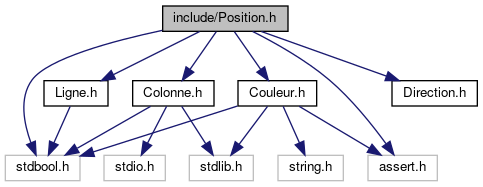
\includegraphics[width=350pt]{Position_8h__incl}
\end{center}
\end{figure}
Ce graphe montre quels fichiers incluent directement ou indirectement ce fichier \+:
\nopagebreak
\begin{figure}[H]
\begin{center}
\leavevmode
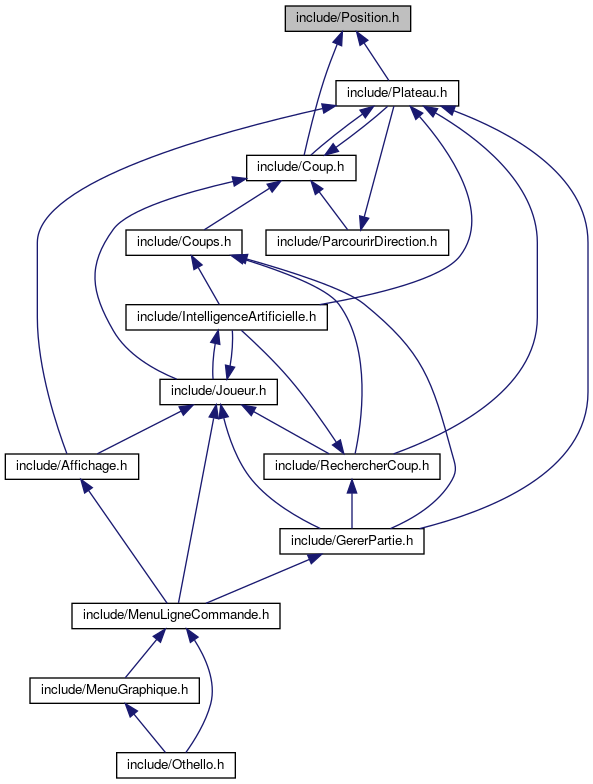
\includegraphics[width=350pt]{Position_8h__dep__incl}
\end{center}
\end{figure}
\subsection*{Classes}
\begin{DoxyCompactItemize}
\item 
struct \hyperlink{structPosition}{Position}
\begin{DoxyCompactList}\small\item\em Le type \hyperlink{structPosition}{Position} permet de symboliser les cases du plateau. \end{DoxyCompactList}\end{DoxyCompactItemize}
\subsection*{Fonctions}
\begin{DoxyCompactItemize}
\item 
\hyperlink{structPosition}{Position} \hyperlink{Position_8h_a61dec4aa9f7fa4d042bbc3b8f1368acb}{P\+O\+S\+I\+T\+I\+O\+N\+\_\+\+Creer\+Position} (\hyperlink{Ligne_8h_a5cdc09714e36ad7319234eab8fdf5e0b}{Ligne} ligne, \hyperlink{Colonne_8h_aae4471c444022e1a2ce4e2af6c2d4419}{Colonne} colonne)
\begin{DoxyCompactList}\small\item\em Crée une \hyperlink{structPosition}{Position}. \end{DoxyCompactList}\item 
\hyperlink{Ligne_8h_a5cdc09714e36ad7319234eab8fdf5e0b}{Ligne} \hyperlink{Position_8h_a433c112916adba44c03861546b634306}{P\+O\+S\+I\+T\+I\+O\+N\+\_\+\+Obtenir\+Ligne} (\hyperlink{structPosition}{Position} position)
\begin{DoxyCompactList}\small\item\em Permet d\textquotesingle{}accéder au champs Ligne de la \hyperlink{structPosition}{Position}. \end{DoxyCompactList}\item 
\hyperlink{Colonne_8h_aae4471c444022e1a2ce4e2af6c2d4419}{Colonne} \hyperlink{Position_8h_ad21b2f29bb972a8f788bd559e1ca06e3}{P\+O\+S\+I\+T\+I\+O\+N\+\_\+\+Obtenir\+Colonne} (\hyperlink{structPosition}{Position} position)
\begin{DoxyCompactList}\small\item\em Permet d\textquotesingle{}accéder au champs Colonne de la \hyperlink{structPosition}{Position}. \end{DoxyCompactList}\item 
void \hyperlink{Position_8h_af8df127d881b60f03c86a8df2572a586}{P\+O\+S\+I\+T\+I\+O\+N\+\_\+\+Fixer\+Ligne} (\hyperlink{structPosition}{Position} $\ast$position, \hyperlink{Ligne_8h_a5cdc09714e36ad7319234eab8fdf5e0b}{Ligne} ligne)
\begin{DoxyCompactList}\small\item\em Permet de modifier le champs Ligne de la \hyperlink{structPosition}{Position}. \end{DoxyCompactList}\item 
void \hyperlink{Position_8h_ab56c68ab09e1d9355661bfdfb900e582}{P\+O\+S\+I\+T\+I\+O\+N\+\_\+\+Fixer\+Colonne} (\hyperlink{structPosition}{Position} $\ast$position, \hyperlink{Colonne_8h_aae4471c444022e1a2ce4e2af6c2d4419}{Colonne} colonne)
\begin{DoxyCompactList}\small\item\em Permet de modifier le champs Colonne de la \hyperlink{structPosition}{Position}. \end{DoxyCompactList}\item 
\hyperlink{structPosition}{Position} \hyperlink{Position_8h_a5a6111c36df5c4f8ac4cde8fe111b16e}{P\+O\+S\+I\+T\+I\+O\+N\+\_\+\+Appliquer\+Direction} (\hyperlink{structPosition}{Position} position, \hyperlink{Direction_8h_a224b9163917ac32fc95a60d8c1eec3aa}{Direction} direction)
\begin{DoxyCompactList}\small\item\em Applique une Direction à la \hyperlink{structPosition}{Position}. \end{DoxyCompactList}\item 
bool \hyperlink{Position_8h_a1dc37e5024770f745b62ff6314493087}{P\+O\+S\+I\+T\+I\+O\+N\+\_\+\+Sont\+Egales\+Positions} (\hyperlink{structPosition}{Position} position1, \hyperlink{structPosition}{Position} position2)
\begin{DoxyCompactList}\small\item\em Détermine si les \hyperlink{structPosition}{Position} sont identiques. \end{DoxyCompactList}\end{DoxyCompactItemize}


\subsection{Description détaillée}
Fichier contenant la définition du type \hyperlink{structPosition}{Position} et de ses fonctions associées. 



\subsection{Documentation des fonctions}
\mbox{\Hypertarget{Position_8h_a5a6111c36df5c4f8ac4cde8fe111b16e}\label{Position_8h_a5a6111c36df5c4f8ac4cde8fe111b16e}} 
\index{Position.\+h@{Position.\+h}!P\+O\+S\+I\+T\+I\+O\+N\+\_\+\+Appliquer\+Direction@{P\+O\+S\+I\+T\+I\+O\+N\+\_\+\+Appliquer\+Direction}}
\index{P\+O\+S\+I\+T\+I\+O\+N\+\_\+\+Appliquer\+Direction@{P\+O\+S\+I\+T\+I\+O\+N\+\_\+\+Appliquer\+Direction}!Position.\+h@{Position.\+h}}
\subsubsection{\texorpdfstring{P\+O\+S\+I\+T\+I\+O\+N\+\_\+\+Appliquer\+Direction()}{POSITION\_AppliquerDirection()}}
{\footnotesize\ttfamily \hyperlink{structPosition}{Position} P\+O\+S\+I\+T\+I\+O\+N\+\_\+\+Appliquer\+Direction (\begin{DoxyParamCaption}\item[{\hyperlink{structPosition}{Position}}]{position,  }\item[{\hyperlink{Direction_8h_a224b9163917ac32fc95a60d8c1eec3aa}{Direction}}]{direction }\end{DoxyParamCaption})}



Applique une Direction à la \hyperlink{structPosition}{Position}. 

Attention, la fontion ne modifie pas la \hyperlink{structPosition}{Position} donnée mais elle renvoi bien une autre \hyperlink{structPosition}{Position} à laquelle on a appliqué la modification.


\begin{DoxyParams}{Paramètres}
{\em position} & \hyperlink{structPosition}{Position} de départ à laquelle on souhaite appliquer une Direction. \\
\hline
{\em direction} & Direction à appliquer sur la \hyperlink{structPosition}{Position}.\\
\hline
\end{DoxyParams}
\begin{DoxyReturn}{Renvoie}
Nouvelle \hyperlink{structPosition}{Position} avec la Direction appliquée. 
\end{DoxyReturn}
\mbox{\Hypertarget{Position_8h_a61dec4aa9f7fa4d042bbc3b8f1368acb}\label{Position_8h_a61dec4aa9f7fa4d042bbc3b8f1368acb}} 
\index{Position.\+h@{Position.\+h}!P\+O\+S\+I\+T\+I\+O\+N\+\_\+\+Creer\+Position@{P\+O\+S\+I\+T\+I\+O\+N\+\_\+\+Creer\+Position}}
\index{P\+O\+S\+I\+T\+I\+O\+N\+\_\+\+Creer\+Position@{P\+O\+S\+I\+T\+I\+O\+N\+\_\+\+Creer\+Position}!Position.\+h@{Position.\+h}}
\subsubsection{\texorpdfstring{P\+O\+S\+I\+T\+I\+O\+N\+\_\+\+Creer\+Position()}{POSITION\_CreerPosition()}}
{\footnotesize\ttfamily \hyperlink{structPosition}{Position} P\+O\+S\+I\+T\+I\+O\+N\+\_\+\+Creer\+Position (\begin{DoxyParamCaption}\item[{\hyperlink{Ligne_8h_a5cdc09714e36ad7319234eab8fdf5e0b}{Ligne}}]{ligne,  }\item[{\hyperlink{Colonne_8h_aae4471c444022e1a2ce4e2af6c2d4419}{Colonne}}]{colonne }\end{DoxyParamCaption})}



Crée une \hyperlink{structPosition}{Position}. 


\begin{DoxyParams}{Paramètres}
{\em ligne} & Ligne de la \hyperlink{structPosition}{Position}. \\
\hline
{\em colonne} & Colonne de la \hyperlink{structPosition}{Position}.\\
\hline
\end{DoxyParams}
\begin{DoxyReturn}{Renvoie}
Instance de \hyperlink{structPosition}{Position}. 
\end{DoxyReturn}
\mbox{\Hypertarget{Position_8h_ab56c68ab09e1d9355661bfdfb900e582}\label{Position_8h_ab56c68ab09e1d9355661bfdfb900e582}} 
\index{Position.\+h@{Position.\+h}!P\+O\+S\+I\+T\+I\+O\+N\+\_\+\+Fixer\+Colonne@{P\+O\+S\+I\+T\+I\+O\+N\+\_\+\+Fixer\+Colonne}}
\index{P\+O\+S\+I\+T\+I\+O\+N\+\_\+\+Fixer\+Colonne@{P\+O\+S\+I\+T\+I\+O\+N\+\_\+\+Fixer\+Colonne}!Position.\+h@{Position.\+h}}
\subsubsection{\texorpdfstring{P\+O\+S\+I\+T\+I\+O\+N\+\_\+\+Fixer\+Colonne()}{POSITION\_FixerColonne()}}
{\footnotesize\ttfamily void P\+O\+S\+I\+T\+I\+O\+N\+\_\+\+Fixer\+Colonne (\begin{DoxyParamCaption}\item[{\hyperlink{structPosition}{Position} $\ast$}]{position,  }\item[{\hyperlink{Colonne_8h_aae4471c444022e1a2ce4e2af6c2d4419}{Colonne}}]{colonne }\end{DoxyParamCaption})}



Permet de modifier le champs Colonne de la \hyperlink{structPosition}{Position}. 


\begin{DoxyParams}{Paramètres}
{\em position} & \hyperlink{structPosition}{Position} dont on souhaite modifier la Colonne. \\
\hline
{\em colonne} & Nouvelle valeur de la Colonne.\\
\hline
\end{DoxyParams}
Permet de modifier le champs Colonne de la \hyperlink{structPosition}{Position}.

\hyperlink{structPosition}{Position} Appliquer\+Direction(\+Position position, Direction direction)\{ \hyperlink{structPosition}{Position} old\+Pos = position; Fixer\+Ligne(\&position, Obtenir\+Ligne(position) + Obtenir\+Decalage\+Ligne(direction)); Fixer\+Colonne(\&position, Obtenir\+Colonne(position) + Obtenir\+Decalage\+Colonne(direction)); if(\+Est\+Position\+Valide(position))\{ return position; \} else\{ return old\+Pos; \} \} \mbox{\Hypertarget{Position_8h_af8df127d881b60f03c86a8df2572a586}\label{Position_8h_af8df127d881b60f03c86a8df2572a586}} 
\index{Position.\+h@{Position.\+h}!P\+O\+S\+I\+T\+I\+O\+N\+\_\+\+Fixer\+Ligne@{P\+O\+S\+I\+T\+I\+O\+N\+\_\+\+Fixer\+Ligne}}
\index{P\+O\+S\+I\+T\+I\+O\+N\+\_\+\+Fixer\+Ligne@{P\+O\+S\+I\+T\+I\+O\+N\+\_\+\+Fixer\+Ligne}!Position.\+h@{Position.\+h}}
\subsubsection{\texorpdfstring{P\+O\+S\+I\+T\+I\+O\+N\+\_\+\+Fixer\+Ligne()}{POSITION\_FixerLigne()}}
{\footnotesize\ttfamily void P\+O\+S\+I\+T\+I\+O\+N\+\_\+\+Fixer\+Ligne (\begin{DoxyParamCaption}\item[{\hyperlink{structPosition}{Position} $\ast$}]{position,  }\item[{\hyperlink{Ligne_8h_a5cdc09714e36ad7319234eab8fdf5e0b}{Ligne}}]{ligne }\end{DoxyParamCaption})}



Permet de modifier le champs Ligne de la \hyperlink{structPosition}{Position}. 


\begin{DoxyParams}{Paramètres}
{\em position} & \hyperlink{structPosition}{Position} dont on souhaite modifier la Ligne. \\
\hline
{\em ligne} & Nouvelle valeur de la Ligne. \\
\hline
\end{DoxyParams}
\mbox{\Hypertarget{Position_8h_ad21b2f29bb972a8f788bd559e1ca06e3}\label{Position_8h_ad21b2f29bb972a8f788bd559e1ca06e3}} 
\index{Position.\+h@{Position.\+h}!P\+O\+S\+I\+T\+I\+O\+N\+\_\+\+Obtenir\+Colonne@{P\+O\+S\+I\+T\+I\+O\+N\+\_\+\+Obtenir\+Colonne}}
\index{P\+O\+S\+I\+T\+I\+O\+N\+\_\+\+Obtenir\+Colonne@{P\+O\+S\+I\+T\+I\+O\+N\+\_\+\+Obtenir\+Colonne}!Position.\+h@{Position.\+h}}
\subsubsection{\texorpdfstring{P\+O\+S\+I\+T\+I\+O\+N\+\_\+\+Obtenir\+Colonne()}{POSITION\_ObtenirColonne()}}
{\footnotesize\ttfamily \hyperlink{Colonne_8h_aae4471c444022e1a2ce4e2af6c2d4419}{Colonne} P\+O\+S\+I\+T\+I\+O\+N\+\_\+\+Obtenir\+Colonne (\begin{DoxyParamCaption}\item[{\hyperlink{structPosition}{Position}}]{position }\end{DoxyParamCaption})}



Permet d\textquotesingle{}accéder au champs Colonne de la \hyperlink{structPosition}{Position}. 


\begin{DoxyParams}{Paramètres}
{\em position} & \hyperlink{structPosition}{Position} dont on souhaite obtenir la Colonne.\\
\hline
\end{DoxyParams}
\begin{DoxyReturn}{Renvoie}
Colonne de la \hyperlink{structPosition}{Position}. 
\end{DoxyReturn}
\mbox{\Hypertarget{Position_8h_a433c112916adba44c03861546b634306}\label{Position_8h_a433c112916adba44c03861546b634306}} 
\index{Position.\+h@{Position.\+h}!P\+O\+S\+I\+T\+I\+O\+N\+\_\+\+Obtenir\+Ligne@{P\+O\+S\+I\+T\+I\+O\+N\+\_\+\+Obtenir\+Ligne}}
\index{P\+O\+S\+I\+T\+I\+O\+N\+\_\+\+Obtenir\+Ligne@{P\+O\+S\+I\+T\+I\+O\+N\+\_\+\+Obtenir\+Ligne}!Position.\+h@{Position.\+h}}
\subsubsection{\texorpdfstring{P\+O\+S\+I\+T\+I\+O\+N\+\_\+\+Obtenir\+Ligne()}{POSITION\_ObtenirLigne()}}
{\footnotesize\ttfamily \hyperlink{Ligne_8h_a5cdc09714e36ad7319234eab8fdf5e0b}{Ligne} P\+O\+S\+I\+T\+I\+O\+N\+\_\+\+Obtenir\+Ligne (\begin{DoxyParamCaption}\item[{\hyperlink{structPosition}{Position}}]{position }\end{DoxyParamCaption})}



Permet d\textquotesingle{}accéder au champs Ligne de la \hyperlink{structPosition}{Position}. 


\begin{DoxyParams}{Paramètres}
{\em position} & \hyperlink{structPosition}{Position} dont on souhaite obtenir la Ligne.\\
\hline
\end{DoxyParams}
\begin{DoxyReturn}{Renvoie}
Ligne de la \hyperlink{structPosition}{Position}. 
\end{DoxyReturn}
\mbox{\Hypertarget{Position_8h_a1dc37e5024770f745b62ff6314493087}\label{Position_8h_a1dc37e5024770f745b62ff6314493087}} 
\index{Position.\+h@{Position.\+h}!P\+O\+S\+I\+T\+I\+O\+N\+\_\+\+Sont\+Egales\+Positions@{P\+O\+S\+I\+T\+I\+O\+N\+\_\+\+Sont\+Egales\+Positions}}
\index{P\+O\+S\+I\+T\+I\+O\+N\+\_\+\+Sont\+Egales\+Positions@{P\+O\+S\+I\+T\+I\+O\+N\+\_\+\+Sont\+Egales\+Positions}!Position.\+h@{Position.\+h}}
\subsubsection{\texorpdfstring{P\+O\+S\+I\+T\+I\+O\+N\+\_\+\+Sont\+Egales\+Positions()}{POSITION\_SontEgalesPositions()}}
{\footnotesize\ttfamily bool P\+O\+S\+I\+T\+I\+O\+N\+\_\+\+Sont\+Egales\+Positions (\begin{DoxyParamCaption}\item[{\hyperlink{structPosition}{Position}}]{position1,  }\item[{\hyperlink{structPosition}{Position}}]{position2 }\end{DoxyParamCaption})}



Détermine si les \hyperlink{structPosition}{Position} sont identiques. 


\begin{DoxyParams}{Paramètres}
{\em position1} & Première \hyperlink{structPosition}{Position} à comparer. \\
\hline
{\em position2} & Seconde \hyperlink{structPosition}{Position} à comparer.\\
\hline
\end{DoxyParams}
\begin{DoxyReturn}{Renvoie}
true si les deux \hyperlink{structPosition}{Position} sont égales, false sinon. 
\end{DoxyReturn}

\hypertarget{RechercherCoup_8h}{}\section{Référence du fichier include/\+Rechercher\+Coup.h}
\label{RechercherCoup_8h}\index{include/\+Rechercher\+Coup.\+h@{include/\+Rechercher\+Coup.\+h}}


Fichier contenant la définition des fonctions pour rechercher des \hyperlink{structCoup}{Coup} possibles.  


{\ttfamily \#include \char`\"{}Coups.\+h\char`\"{}}\newline
{\ttfamily \#include \char`\"{}Joueur.\+h\char`\"{}}\newline
{\ttfamily \#include \char`\"{}Plateau.\+h\char`\"{}}\newline
Graphe des dépendances par inclusion de Rechercher\+Coup.\+h\+:
\nopagebreak
\begin{figure}[H]
\begin{center}
\leavevmode
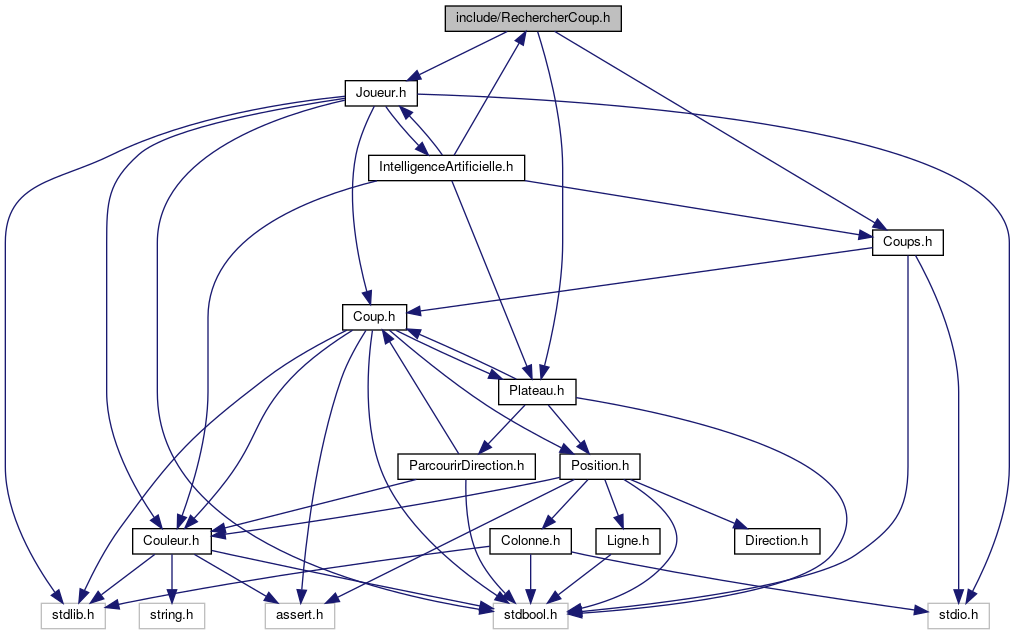
\includegraphics[width=350pt]{RechercherCoup_8h__incl}
\end{center}
\end{figure}
Ce graphe montre quels fichiers incluent directement ou indirectement ce fichier \+:
\nopagebreak
\begin{figure}[H]
\begin{center}
\leavevmode
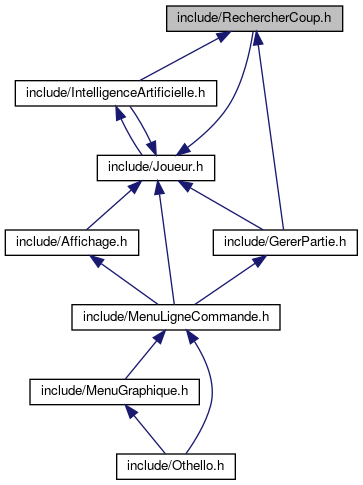
\includegraphics[width=344pt]{RechercherCoup_8h__dep__incl}
\end{center}
\end{figure}
\subsection*{Fonctions}
\begin{DoxyCompactItemize}
\item 
\hyperlink{structCoups}{Coups} \hyperlink{RechercherCoup_8h_ad59177f1b310f336282e9b2e057040be}{R\+E\+C\+H\+E\+R\+C\+H\+E\+C\+O\+U\+P\+\_\+\+Rechercher\+Tous\+Les\+Coups} (\hyperlink{structCouleur}{Couleur} $\ast$plateau, \hyperlink{structCouleur}{Couleur} couleur)
\begin{DoxyCompactList}\small\item\em Crée une instance de \hyperlink{structCoups}{Coups} avec tous les \hyperlink{structCoup}{Coup} possibles pour une \hyperlink{structCouleur}{Couleur} donnée. \end{DoxyCompactList}\item 
bool \hyperlink{RechercherCoup_8h_aeb5d45b2a3abcad075307ffa24ad4f35}{R\+E\+C\+H\+E\+R\+C\+H\+E\+C\+O\+U\+P\+\_\+\+Est\+Coup\+Valide} (\hyperlink{structCouleur}{Couleur} $\ast$plateau, \hyperlink{structCoup}{Coup} coup)
\begin{DoxyCompactList}\small\item\em Détermine si un \hyperlink{structCoup}{Coup} est valide. \end{DoxyCompactList}\item 
\hyperlink{structCoup}{Coup} \hyperlink{RechercherCoup_8h_adb221d5ef4627cf594c925c81d449bbc}{R\+E\+C\+H\+E\+R\+C\+H\+E\+C\+O\+U\+P\+\_\+\+Obtenir\+Coup\+Valide} (\hyperlink{structCouleur}{Couleur} $\ast$plateau, \hyperlink{structJoueur}{Joueur} joueur)
\begin{DoxyCompactList}\small\item\em Permet d\textquotesingle{}obtenir un \hyperlink{structCoup}{Coup} forcément valide de la part d\textquotesingle{}un \hyperlink{structJoueur}{Joueur}. \end{DoxyCompactList}\end{DoxyCompactItemize}


\subsection{Description détaillée}
Fichier contenant la définition des fonctions pour rechercher des \hyperlink{structCoup}{Coup} possibles. 



\subsection{Documentation des fonctions}
\mbox{\Hypertarget{RechercherCoup_8h_aeb5d45b2a3abcad075307ffa24ad4f35}\label{RechercherCoup_8h_aeb5d45b2a3abcad075307ffa24ad4f35}} 
\index{Rechercher\+Coup.\+h@{Rechercher\+Coup.\+h}!R\+E\+C\+H\+E\+R\+C\+H\+E\+C\+O\+U\+P\+\_\+\+Est\+Coup\+Valide@{R\+E\+C\+H\+E\+R\+C\+H\+E\+C\+O\+U\+P\+\_\+\+Est\+Coup\+Valide}}
\index{R\+E\+C\+H\+E\+R\+C\+H\+E\+C\+O\+U\+P\+\_\+\+Est\+Coup\+Valide@{R\+E\+C\+H\+E\+R\+C\+H\+E\+C\+O\+U\+P\+\_\+\+Est\+Coup\+Valide}!Rechercher\+Coup.\+h@{Rechercher\+Coup.\+h}}
\subsubsection{\texorpdfstring{R\+E\+C\+H\+E\+R\+C\+H\+E\+C\+O\+U\+P\+\_\+\+Est\+Coup\+Valide()}{RECHERCHECOUP\_EstCoupValide()}}
{\footnotesize\ttfamily bool R\+E\+C\+H\+E\+R\+C\+H\+E\+C\+O\+U\+P\+\_\+\+Est\+Coup\+Valide (\begin{DoxyParamCaption}\item[{\hyperlink{structCouleur}{Couleur} $\ast$}]{plateau,  }\item[{\hyperlink{structCoup}{Coup}}]{coup }\end{DoxyParamCaption})}



Détermine si un \hyperlink{structCoup}{Coup} est valide. 

On admet un \hyperlink{structCoup}{Coup} valide un \hyperlink{structCoup}{Coup} dont la \hyperlink{structPosition}{Position} est valide, dont la \hyperlink{structPosition}{Position} est libre, et qui permet de capturer au moins 1 pion.


\begin{DoxyParams}{Paramètres}
{\em plateau} & Plateau de jeu. \\
\hline
{\em coup} & \hyperlink{structCoup}{Coup} dont on souhaite déterminer la validité.\\
\hline
\end{DoxyParams}
\begin{DoxyReturn}{Renvoie}
true si le \hyperlink{structCoup}{Coup} est valide, false sinon. 
\end{DoxyReturn}
\mbox{\Hypertarget{RechercherCoup_8h_adb221d5ef4627cf594c925c81d449bbc}\label{RechercherCoup_8h_adb221d5ef4627cf594c925c81d449bbc}} 
\index{Rechercher\+Coup.\+h@{Rechercher\+Coup.\+h}!R\+E\+C\+H\+E\+R\+C\+H\+E\+C\+O\+U\+P\+\_\+\+Obtenir\+Coup\+Valide@{R\+E\+C\+H\+E\+R\+C\+H\+E\+C\+O\+U\+P\+\_\+\+Obtenir\+Coup\+Valide}}
\index{R\+E\+C\+H\+E\+R\+C\+H\+E\+C\+O\+U\+P\+\_\+\+Obtenir\+Coup\+Valide@{R\+E\+C\+H\+E\+R\+C\+H\+E\+C\+O\+U\+P\+\_\+\+Obtenir\+Coup\+Valide}!Rechercher\+Coup.\+h@{Rechercher\+Coup.\+h}}
\subsubsection{\texorpdfstring{R\+E\+C\+H\+E\+R\+C\+H\+E\+C\+O\+U\+P\+\_\+\+Obtenir\+Coup\+Valide()}{RECHERCHECOUP\_ObtenirCoupValide()}}
{\footnotesize\ttfamily \hyperlink{structCoup}{Coup} R\+E\+C\+H\+E\+R\+C\+H\+E\+C\+O\+U\+P\+\_\+\+Obtenir\+Coup\+Valide (\begin{DoxyParamCaption}\item[{\hyperlink{structCouleur}{Couleur} $\ast$}]{plateau,  }\item[{\hyperlink{structJoueur}{Joueur}}]{joueur }\end{DoxyParamCaption})}



Permet d\textquotesingle{}obtenir un \hyperlink{structCoup}{Coup} forcément valide de la part d\textquotesingle{}un \hyperlink{structJoueur}{Joueur}. 


\begin{DoxyParams}{Paramètres}
{\em plateau} & Plateau de jeu. \\
\hline
{\em joueur} & \hyperlink{structJoueur}{Joueur} dont on souhaite obtenir le \hyperlink{structCoup}{Coup}.\\
\hline
\end{DoxyParams}
\begin{DoxyReturn}{Renvoie}
Instance de \hyperlink{structCoup}{Coup} obtenue par la saisie. 
\end{DoxyReturn}
\mbox{\Hypertarget{RechercherCoup_8h_ad59177f1b310f336282e9b2e057040be}\label{RechercherCoup_8h_ad59177f1b310f336282e9b2e057040be}} 
\index{Rechercher\+Coup.\+h@{Rechercher\+Coup.\+h}!R\+E\+C\+H\+E\+R\+C\+H\+E\+C\+O\+U\+P\+\_\+\+Rechercher\+Tous\+Les\+Coups@{R\+E\+C\+H\+E\+R\+C\+H\+E\+C\+O\+U\+P\+\_\+\+Rechercher\+Tous\+Les\+Coups}}
\index{R\+E\+C\+H\+E\+R\+C\+H\+E\+C\+O\+U\+P\+\_\+\+Rechercher\+Tous\+Les\+Coups@{R\+E\+C\+H\+E\+R\+C\+H\+E\+C\+O\+U\+P\+\_\+\+Rechercher\+Tous\+Les\+Coups}!Rechercher\+Coup.\+h@{Rechercher\+Coup.\+h}}
\subsubsection{\texorpdfstring{R\+E\+C\+H\+E\+R\+C\+H\+E\+C\+O\+U\+P\+\_\+\+Rechercher\+Tous\+Les\+Coups()}{RECHERCHECOUP\_RechercherTousLesCoups()}}
{\footnotesize\ttfamily \hyperlink{structCoups}{Coups} R\+E\+C\+H\+E\+R\+C\+H\+E\+C\+O\+U\+P\+\_\+\+Rechercher\+Tous\+Les\+Coups (\begin{DoxyParamCaption}\item[{\hyperlink{structCouleur}{Couleur} $\ast$}]{plateau,  }\item[{\hyperlink{structCouleur}{Couleur}}]{couleur }\end{DoxyParamCaption})}



Crée une instance de \hyperlink{structCoups}{Coups} avec tous les \hyperlink{structCoup}{Coup} possibles pour une \hyperlink{structCouleur}{Couleur} donnée. 


\begin{DoxyParams}{Paramètres}
{\em plateau} & Plateau de jeu. \\
\hline
{\em couleur} & \hyperlink{structCouleur}{Couleur} du \hyperlink{structJoueur}{Joueur} dont on souhaite trouver les \hyperlink{structCoups}{Coups}.\\
\hline
\end{DoxyParams}
\begin{DoxyReturn}{Renvoie}
Instance de \hyperlink{structCoups}{Coups}. 
\end{DoxyReturn}

\chapter{Documentation des exemples}
\hypertarget{COLONNE_ObtenirColonneDepuisChar-example}{}\section{C\+O\+L\+O\+N\+N\+E\+\_\+\+Obtenir\+Colonne\+Depuis\+Char}
Obtient la Colonne correspondante à un caractère.(\textquotesingle{}d\textquotesingle{}) = Colonne d


\begin{DoxyParams}{Paramètres}
{\em char} & Caractère dont on souhaite retrouver la Colonne.\\
\hline
\end{DoxyParams}
\begin{DoxyReturn}{Renvoie}
Enumeration Colonne correspond au caractère.
\end{DoxyReturn}

\begin{DoxyCodeInclude}
\end{DoxyCodeInclude}
 
\hypertarget{COLONNE_ObtenirColonneDepuisInt-example}{}\section{C\+O\+L\+O\+N\+N\+E\+\_\+\+Obtenir\+Colonne\+Depuis\+Int}
Obtient la Colonne correspondante à un integer.(2) =$>$ Colonne b


\begin{DoxyParams}{Paramètres}
{\em int} & Numéro dont on souhaite retrouver la Colonne.\\
\hline
\end{DoxyParams}
\begin{DoxyReturn}{Renvoie}
Enumeration Colonne correspondant au numéro.
\end{DoxyReturn}

\begin{DoxyCodeInclude}
\end{DoxyCodeInclude}
 
\hypertarget{COLONNE_ObtenirNumeroColonne-example}{}\section{C\+O\+L\+O\+N\+N\+E\+\_\+\+Obtenir\+Numero\+Colonne}
Obtient le numero réel d\textquotesingle{}une Colonne. L\textquotesingle{}énumeration en C commence à 0 alors que nous travaillons avec des ligne et des Colonne dont les indices commencent à 1.

(a) = 1


\begin{DoxyParams}{Paramètres}
{\em colonne} & Colonne dont on souhaite obtenir le numéro.\\
\hline
\end{DoxyParams}
\begin{DoxyReturn}{Renvoie}
Numéro de la Colonne.
\end{DoxyReturn}

\begin{DoxyCodeInclude}
\end{DoxyCodeInclude}
 
\hypertarget{COULEUR_ObtenirCouleurOpposee-example}{}\section{C\+O\+U\+L\+E\+U\+R\+\_\+\+Obtenir\+Couleur\+Opposee}
Retourne la \hyperlink{structCouleur}{Couleur} opposée à celle passée en entrée.(instance\+Noir) = instance\+Blanc


\begin{DoxyParams}{Paramètres}
{\em couleur} & \hyperlink{structCouleur}{Couleur} dont on souhaite obtenir la couleur opposée.\\
\hline
\end{DoxyParams}
\begin{DoxyReturn}{Renvoie}
Instance de la \hyperlink{structCouleur}{Couleur} opposée à celle passée en entrée.
\end{DoxyReturn}

\begin{DoxyCodeInclude}
\end{DoxyCodeInclude}
 
\hypertarget{LIGNE_ObtenirLigneDepuisInt-example}{}\section{L\+I\+G\+N\+E\+\_\+\+Obtenir\+Ligne\+Depuis\+Int}
Obtient la Ligne correspondante à un integer.(3) =$>$ ligne Trois


\begin{DoxyParams}{Paramètres}
{\em int} & Numéro dont on souhaite retrouver la Ligne.\\
\hline
\end{DoxyParams}
\begin{DoxyReturn}{Renvoie}
Enumeration Ligne correspondant au numéro.
\end{DoxyReturn}

\begin{DoxyCodeInclude}
\end{DoxyCodeInclude}
 
\hypertarget{LIGNE_ObtenirNumeroLigne-example}{}\section{L\+I\+G\+N\+E\+\_\+\+Obtenir\+Numero\+Ligne}
Obtient le numero réel d\textquotesingle{}une Ligne. L\textquotesingle{}énumeration en C commence à 0 alors que nous travaillons avec des Ligne et des Colonne dont les indices commencent à 1.

(Un) = 1


\begin{DoxyParams}{Paramètres}
{\em ligne} & Ligne dont on souhaite obtenir le numéro.\\
\hline
\end{DoxyParams}
\begin{DoxyReturn}{Renvoie}
Numéro de la Ligne.
\end{DoxyReturn}

\begin{DoxyCodeInclude}
\end{DoxyCodeInclude}
 
\hypertarget{PARTIE_FaireUnePartie-example}{}\section{P\+A\+R\+T\+I\+E\+\_\+\+Faire\+Une\+Partie}
Permet de lancer une partie. Cette fonction initialise le plateau de jeu et lance le jeu.

(Afficher\+Resultat,Afficher\+Plateau,Afficher\+Coup, Afficher\+Saisie\+Coup, j1,j2)


\begin{DoxyParams}{Paramètres}
{\em Afficher\+Resultat} & Pointeur de fonction pour afficher les resultats de la partie. \\
\hline
{\em Afficher\+Plateau} & Pointeur de fonction pour afficher le plateau. \\
\hline
{\em Afficher\+Coup} & Pointeur de fonction pour afficher le coup qui viens d\textquotesingle{}être joué \\
\hline
{\em Afficher\+Saisie\+Coup} & Pointeur de fonction pour afficher la demande de saisie d\textquotesingle{}un coup \\
\hline
{\em j1} & Premier \hyperlink{structJoueur}{Joueur}. \\
\hline
{\em j2} & Second \hyperlink{structJoueur}{Joueur}.\\
\hline
\end{DoxyParams}

\begin{DoxyCodeInclude}
\end{DoxyCodeInclude}
 
\hypertarget{PLATEAU_InitialiserPlateau-example}{}\section{P\+L\+A\+T\+E\+A\+U\+\_\+\+Initialiser\+Plateau}
Initialise un plateau de jeu avec 4 cases du centre remplies et les autres neutres.(p) = le plateau p initialisé


\begin{DoxyParams}{Paramètres}
{\em plateau} & Plateau de jeu\\
\hline
\end{DoxyParams}

\begin{DoxyCodeInclude}
\end{DoxyCodeInclude}
 
%--- End generated contents ---

% Index
\backmatter
\newpage
\phantomsection
\clearemptydoublepage
\addcontentsline{toc}{chapter}{Index}
\printindex

\end{document}
